\chapter{Introduction}

Deefake is the buzzword that has no agreed-upon technical definition. It consists of two words, deep and fake. Deep is referring to deep learning machine learning, which is used for creating fake voices, images, or even videos. It is a fast growing technical field of study and could be a major threat to society. We live in information era and creation of unrecognizable fake media affects us all. Deepfakes could be found on social media, news portals, etc.

This paper shows some security risks and impacts on many different fields of human life. There are already many popular videos containing deepfakes on social networks with millions of views, but also several successful attacks on biometrics systems. People are not able to consistently recognize deepfakes. That is why we need to create detection tools to help anyone with problem that is already there.

There are many different deepfake categories from face swap to face morphing and more. Most of the detection methods focus on a single domain, which means that they are capable of detecting only one deepfake category. There are few tools in the market utilizing those detection methods targeting undemanding/inexperienced users, and some of them are not free to use.

The first two chapters cover general knowledge about deepfakes such as potential risks and security impacts with mention of successful attacks, different types of voice, image, and video deepfakes. You can read about experimental detection methods and available tools in the market.

Second and more important part describes process of development deepfake detection framework and client application, which is the goal of this work. It starts by specifying requirements followed by detailed architecture. Architecture was designed with focus to easily integrates new detection methods into framework.

Last but not least, the implemented framework containing several open source detection methods was deployed into Azure AKS cluster and properly tested. The tests were mostly focused on the testing framework itself, mostly measuring used resources. Integrated detection methods were also tested, and all the results could be found at the end of this paper.

% ----------------------------------------------------------------------- %
\chapter{Security impacts of deepfakes}

The creation of fake media and their detection have been a problem since photography was invented. Digital photography or video with tools such as GIMP, Adobe Photoshop or Adobe After Effects allows more people to create fakes than before, still some experience in this area is needed. Media that have been modified or otherwise manipulated are called synthetic media, and they do not depend on whether it is an analogue or digital medium. Deepfakes also fall under this category~\cite{IncreasingThreatofDeepfakeIdentites}. Deep learning-powered tools allow even more unexperienced users to easily create trustworthy fakes. 

The quality of deepfakes reached a level when a trained person or even an experienced researcher in this field has a problem of spotting them. This fast development allows creating realistically looking assets to art photography or movie production; unfortunately, it can be used for malicious purposes like creating fake porn videos to blackmail people or manipulate public via fake news. There are many use cases where deepfakes can be applied.

This is not a discussion about potential technology; deepfakes are already there and their usage will probably have an increasing trend. Over the last couple months, we could see huge development and popularity explosion around large language models such as ChatGPT~\cite{ ChatGPTPopularity}. Deepfakes do not have such publicity, but they have the same potential to change whole human society as previously mentioned language models. We are not far from using a pre-trained voice deepfake model powered by some large language model to automatically perform attack itself.

It is putting huge pressure on researchers to develop new forensics tools or any technology which will prevent malicious usage of deepfakes. As mentioned before, creating fakes is not new, and a whole field of study engaged in spotting fakes and developing techniques over 15 years. Despite continuous research efforts in the past, the advent of deep learning changed the rules of the game.~\cite{MediaForensicsandDeepFakes}

\section{Human capabilities of deepfake detection}

The human ability to recognize fake materials from the originals is in contradiction to their quality. Korshunov and Marcel \cite{TheThreatOfDeepfakes} confirmed this in their research. They created a questionnaire containing several videos, and the subject (interviewee) had to answer after watching the video whether the person in the video was genuine, fake, or uncertain. The videos were manually divided into five categories (very easy, easy, moderate, difficult, and very difficult, original). 

The videos were split into several categories manually by the researchers, probably without using any metrics but based on their experience and feelings. Afterwards, ANOVA test shows there is an overlap in several categories, so several videos could be moved to a different category. However, the categories are still significantly different.

The results of test in fig.~\ref{fig:subjective_answers} certainly demonstrate that people's recognition ability decreases significantly as the quality of deepfakes increases. Also, the audience of this test knows they are looking for fakes, otherwise we can expect worse results if there will be unsuspected audience (e.g., deepfakes on social media). It is quite alarming that the correct answers in the category of “very easy” reach only 71,1 \%. The quality of deepfake increases over time, thus it can be expected that human recognition ability will continue to decrease. \cite{TheThreatOfDeepfakes}

\begin{figure}[H]
    \begin{subfigure}[h]{0.4985\linewidth}
        \centering
        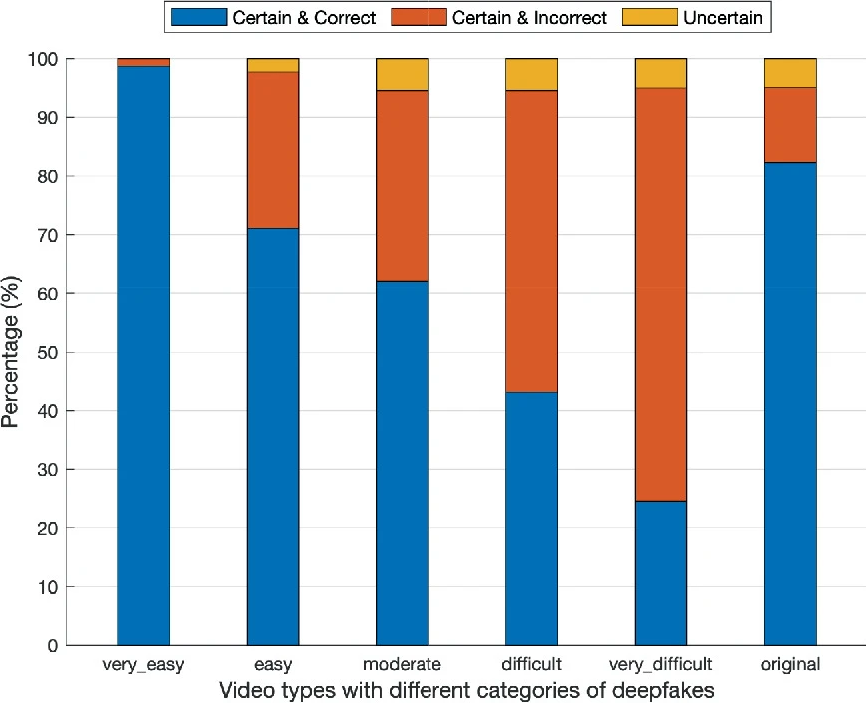
\includegraphics[width=1\linewidth]{other-fig/subjective_answers_a.png}
        \caption{Subjective answers}
    \end{subfigure}
    \hfill
    \begin{subfigure}[h]{0.4985\linewidth}
        \centering
        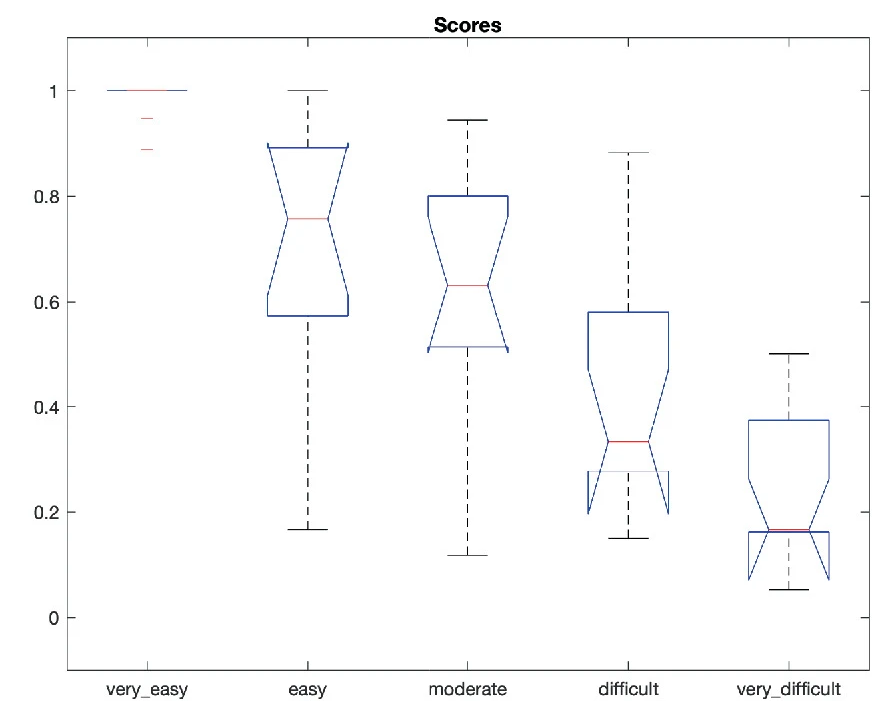
\includegraphics[width=1\linewidth]{other-fig/subjective_answers_b.png}
        \caption{ANOVA test}
    \end{subfigure}
    \caption{Subjective answers and median values with error bars from ANOVA test for different deepfake categories. Retrieved from~\cite{TheThreatOfDeepfakes}.}
    \label{fig:subjective_answers}
\end{figure}

Another research tested only recognition of audio tracks and they were comparing humans versus computer programs. Attendees had a correct classification between fakes and origins 67 \% after the first several rounds. Their accuracy increased while listening and answering to more tracks, but the value stabilizes at 80 \%. On average, trained AI performs about 10 \% better than human, but this result highly depends on the difference in learning and test dataset. Still, it shows that the computer can outperform humans in spotting deepfakes. \cite{HumanPerceptionAudio}

\section{Potentional risks and impacts}

Humans are not good at recognizing deepfakes, but “why should we be worried?”. Almost every technology humankind created could be used for good or bad – deepfake is no exception. There are plenty different deepfake categories, and each has its own attack vector or use case. This section is covering potential risks of those categories and their closer description will be covered in chapter~\ref{chapter:deepfakes_creation}.

Deepfakes are about gaining someone’s trust or influencing him. For the last couple of years, there has been an increasing trend of scamming people, mostly via phone or computer~\cite{HybridVishingAttacksSkyrocketing}. Targeting only one person/victim, for example, to gain their money or information. Those attacks are getting better and more credible and using deepfake to impersonate close friend of victim could be next step how to improve it, if it is not already happening.

Creating “fake news” to influence a large audience is the most common use case of deepfakes because we live in an information era. There are many targets of “fake news” such as rigging elections, demoralizing military units, or manipulating the stock market. In this case, politicians, celebrities, and significant personalities will be used in deepfakes to influence the audience. We can only imagine what one person or a high quality deepfake can change with enough media reach. For example, after one tweet from Elon Musk about Tesla’s stock, sends shares down more than 10 \% almost immediately~\cite{ElonMusksTweets}.~\cite{IncreasingThreatofDeepfakeIdentites}

A real example of deepfake is the famous video with Barak Obama insulting Donald Trump, which should spread awareness regarding the fast developing category of new thread\footnote{\url{https://www.buzzfeed.com/craigsilverman/obama-jordan-peele-deepfake-video-debunk-buzzfeed}}. Several years later another video stating Volodimir Zelenskyj talking about surrendering, it was proved that it is a manipulated video, and its purpose was to demoralize Ukraine army and make them capitulate\footnote{\url{https://www.youtube.com/watch?v=X17yrEV5sl4}}.

There are other videos similar to the video of Barack Obama with the same purpose, spreading awareness about deepfake. For example, speech of Czech Republic president Miloš Zeman created by HBO for propagating their new series\footnote{\url{https://www.youtube.com/watch?v=FzMnDwpKJrI}}, but also to inform general public about this technology. We can consider those videos and their goal to be mostly success. Most people have heard about deepfakes and they are connecting them with those types of videos. However, many people share deepfakes inadvertently on their social media~\cite{DeepfakeSharing}.

Not everyone considered them as a big thread. This is probably because there is no proof that there was a successful deepfake attack or fake news that influence them directly. This is the reason why deepfake could be so dangerous. The video of Volodimir Zelenskyj might have had a good chance to be successful, but it was quite fast debunked because of its terrible quality. People still should be inform about capabilities of deepfakes, but the target of the message should be different. Not saying only be careful we can make politicians say what we want, but show and provide some tools on how to spot the deepfakes.

Another field where deepfakes could be used is to trick biometrics systems to mark attacker as a different person. This technique is used to gain access to secured equipment, to building or even to application (internet banking), etc. Biometrics systems have been proven not ready to deal with deepfakes~\cite{DawnOfTextDependentSociety}~\cite{TheMagicPassport}. The work describing one of attacks is called magic passport and demonstrates how biometric systems could be vulnerable. Most systems will require some changes such as adding a new module to the authentication pipeline, which will be detecting deepfakes~\cite{DigitalFaceManipulation}. Face or voice biometrics recognition systems are in greatest danger. Falsification of documents is related to this topic and there was a case of smuggling people across borders with an official passport containing morphed photos of two individuals~\cite{FaceMorphingAttackDetectionMethods}.

These cases are only the tip of the iceberg, and in the future, everyone should ask if video on social media with film celebrities is real or even worse, if the evidence in courts is trustworthy or not. The solution to this is to use tools capable of detecting deepfakes. Those tools must be created with caution for unskilled users.

\section{Detection tools requirements}

Now we know that deepfakes could be security threats and there is a need for reliable detection tools. There is not many detection tool available for users. Most of them are basically command line scripts which are not for general purpose. More about individual methods could be fined in chapter~\ref{chapter:deepfake_detectoin}.

The user interface should be simple, yet provide all relevant information. Generalizing anything to one number will be great, but not every time it is possible. Speaking of detection methods it should be able to deliver only one number. On the other hand, it will be nice to show the user where on the image is the manipulated area. 

Nowadays people work with many different types of files. Only for audio we can have WAV, OGG, MP3 and many more. This means that the detection method supporting only one file type will not have huge success. There are two types of solution to this problem; first is to support as many file types as possible natively. The second approach will be to utilize existing tools to convert input files to one specific format.

In the end how do we compere different detection methods or even the same methods trained on different datasets. We would have to test each method individually and compare the results manually. There are some problems that need to be sorted out before we will have a reliable detection tool in the market. 

% ----------------------------------------------------------------------- %
\chapter{Types of deepfakes}
\label{chapter:deepfakes_creation}

There are plenty of methods on how to create deepfakes, and as its name suggests some of them are based on deep neural networks but not exclusively. This section describes most common types of neural networks used for creating voice, image, or video deepfakes. One of the most popular types for face deepfakes is Generative adversarial network (GAN), and it is used to create completely new faces or face manipulations.

Each method leaves traces in the medium that can then be detected. This is one way to recognize deepfakes so understanding process of creation is an advantage. Detection is described in more detail in chapter~\ref{chapter:deepfake_detectoin}.

\subsection{Neural networks}

Neural networks are composited from neurons arranged in layers, and each layer is connected sequentially via synapses. Synapses are weighed, and the process of finding the proper value of all weights is called a learning neural network. To obtain results from the input of \(n\)-dimensional \(x\) process \texttt{forward-propagation} is used to propagate \(x\) through each layer.~\cite{CreationandDetectionofDeepfakes}

Input to layer is vector \(a\) of values calculated by previous layer or in case of first layer \(x\) itself. That means result of each layer is also vector calculated by activation function \(f(a*W+b)\), where \(f\) is activation function (Sigmod, ReLU, etc.), \(a\) is input vector, \(W\) is matrix of weights between layers \(i\) and \(i+1\) and b is dimensional bias. Dimensional bias is a constant offset that helps the network shift the activation function toward the positive or negative side~\cite{NeuralNetworkBias}.~\cite{CreationandDetectionofDeepfakes}

Now let’s consider the neural network \(M\) as a black box and denote its execution as \(M(x) = y\). Supervise learning to train \(M\) is using paired samples with from \((x_i, y_i)\) and loss function \(L\) is defined. Loss function is to generate a signal at the output of \(M\) and propagate him back to find error of each weight in synapses.~\cite{CreationandDetectionofDeepfakes}

Optimalization algorithms such as gradient descent are then used to calculate new weights of \(M\) for the number of epochs. As a result of this process, the network learns the function \(M(x_i) \approx y_i\) and is capable of making prediction on unseen data. More detailed descriptions of this could be found in the work of Y. Mirsky and W. Lee~\cite{CreationandDetectionofDeepfakes}.~\cite{CreationandDetectionofDeepfakes}
\\\\
Next list shows types of neural networks used for generating deepfakes~\cite{CreationandDetectionofDeepfakes}:

\begin{itemize}
    \item Generative Adversarial Networks (GAN) – Consist of two neural networks working against each other. One layer is generator and second is discriminator. Generator producing fake features trying to fool discriminator, on the other hand, discriminator is learning to distinguish between real sample and fake one.
    \item Encoder-Decoder networks (ED) – Contains at least two networks, encoder and decoder. It has narrowed layers towards its center. If encoder \(En\) and decoder \(De\) are symmetric and they are trained as \(De(En(x)) = x\), then the network is called autoencoder. Generating deepfakes using ED trained with function \(De(En(x)) = x_g\), where \(x_g\) is fake generated features. There is possibility to use multiple different ED chained after each other or using specific variant of ED called variational autoencoder.
    \item Convolutional Neural Network (CNN) – CNN is learning pattern hierarchies in the data. For deepfakes purposes, it learns filters applied over the input and forming an abstract feature map as the output.
    \item Recurrent Neural Networks (RNN) – RNN can handle variable length data and during processing it remembers state that can be used in next iteration. RNN are mostly used in audio.
\end{itemize}

Each architecture has its own subcategories that have small modifications or using some techniques from different architecture. All above mentioned neural networks types are shown in~\ref{fig:nns_architecture} and~\ref{fig:cnn_architecture} 

\begin{figure}[H]
    \centering
    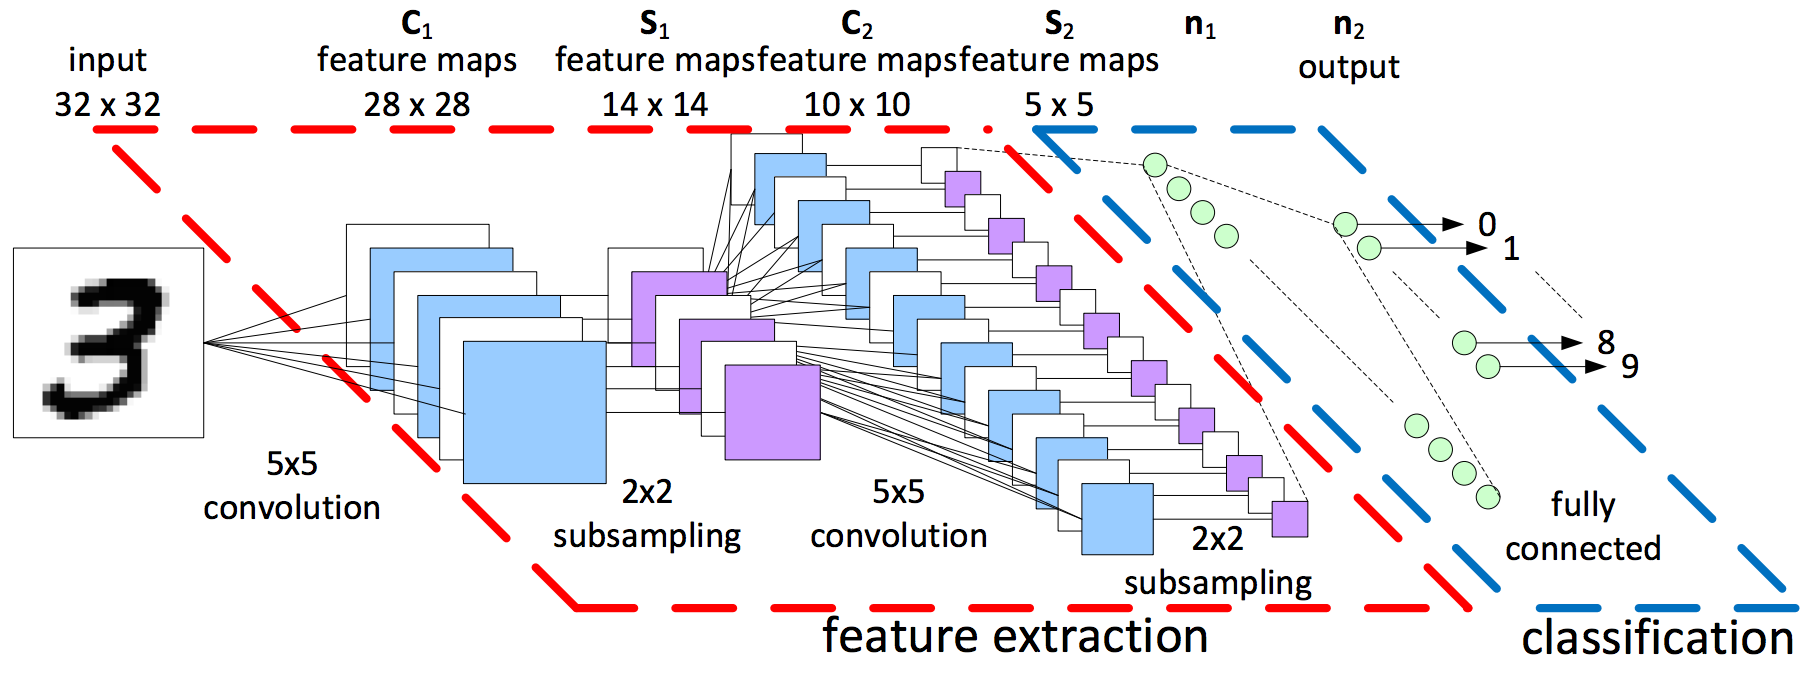
\includegraphics[width=.7\linewidth]{other-fig/cnn.png}
    \caption{Architecture of convolutional neural network. Retrieved from~\cite{CNNArchitecture}.}
    \label{fig:nns_architecture}
\end{figure}

\begin{figure}[H]
    \centering
    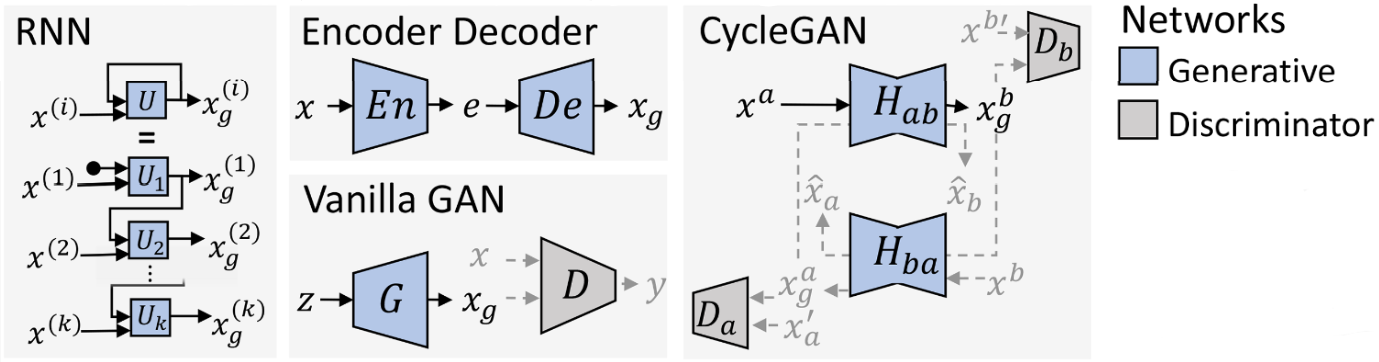
\includegraphics[width=.65\linewidth]{other-fig/nns.png}
    \caption{Basic neural network architectures (RNN, ED, GAN). Retrieved from~\cite{CreationandDetectionofDeepfakes}.}
    \label{fig:cnn_architecture}
\end{figure}

\subsection{Voice deepfakes}

There are three different modalities for speech synthesis: text-to-speech (TTS), voice cloning (VC), and replay attack (RA)~\cite{Deepsonar}. The last one is based on capturing victim voice and the replay of it. It is quite easy and cheap to perform because it only requires capture and replay device (today we can use for example smartphone) and current methods for voice recognition still have accuracy issues~\cite{ReplayAttackDetection}. First two are using AI-synthesis with content regeneration which makes them more indistinguishable for naked ears.~\cite{Deepsonar}

Text to speech (TTS) converts written text to artificial speech, on the other hand voice cloning consumes source voice. Both methods produce synthesis voice saying desired phrases specified by the input, high-level diagram how those methods works could be seen on fig.~\ref{fig:tts_vs}. Voice deepfakes are used independently or with deepfake video (e.g., full puppet). Creating synthesis voice is computationally challenging and one of the goals is making real-time voice cloning. There are several projects that are trying to accomplish this\footnote{\url{https://github.com/SolomidHero/real-time-voice-conversion}} \footnote{\url{https://www.resemble.ai/speech-to-speech/}}.

\begin{figure}[H]
    \centering
    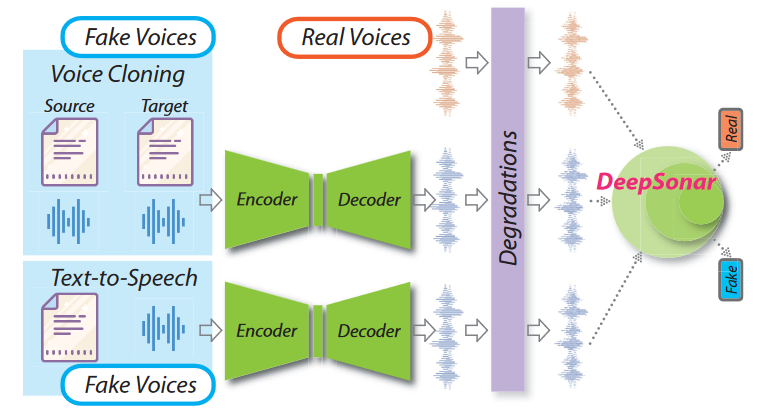
\includegraphics[width=.62\linewidth]{other-fig/tts_vc.png}
    \caption{Text-to-speech and voice cloning data flow diagram. Retrieved from~\cite{Deepsonar}.}
    \label{fig:tts_vs}
\end{figure}

\subsection{Image or video deepfakes}

The list of the following deepfakes is based on the work R. Tolosana, et al.~\cite{IntroductionToDigitalFaceManipulation}:

\begin{itemize}
    \item Identity swap – Replacing the face of subject with the face of target as shown in fig.~\ref{fig:idenity_swap}. There are two different approaches, classical computer graphics-based technique and deep learning technique. Generally, the process of swap could be described as face detection, cropping, extraction of intermediate representations, synthesis of new face, and blending the generated face.
    \begin{figure}[H]
        \centering
        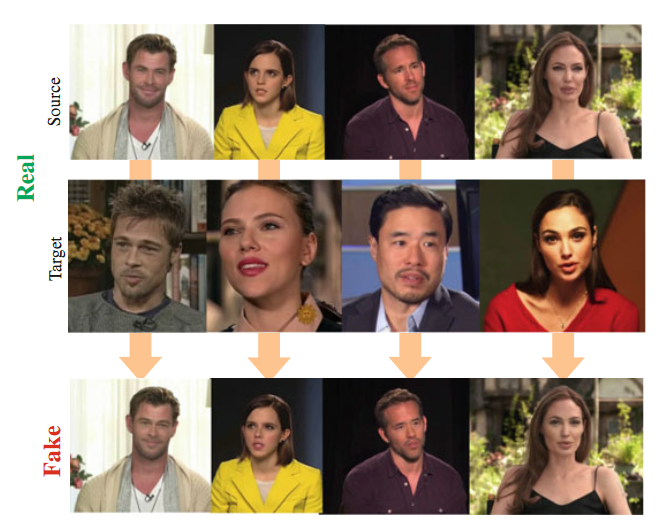
\includegraphics[width=.53\linewidth]{other-fig/idenity_swap.png}
        \caption{Examples of real and fake identity swap images. Retrieved from~\cite{IntroductionToDigitalFaceManipulation}.}
        \label{fig:idenity_swap}
    \end{figure}

    \item Full puppet – Method related to identity swap allows creation of so-called puppet. One person (master) is source of facial expression and body movements that are mapped onto target person as shown in fig.~\ref{fig:full_puppet}.~\cite{IncreasingThreatofDeepfakeIdentites}
    \begin{figure}[H]
        \centering
        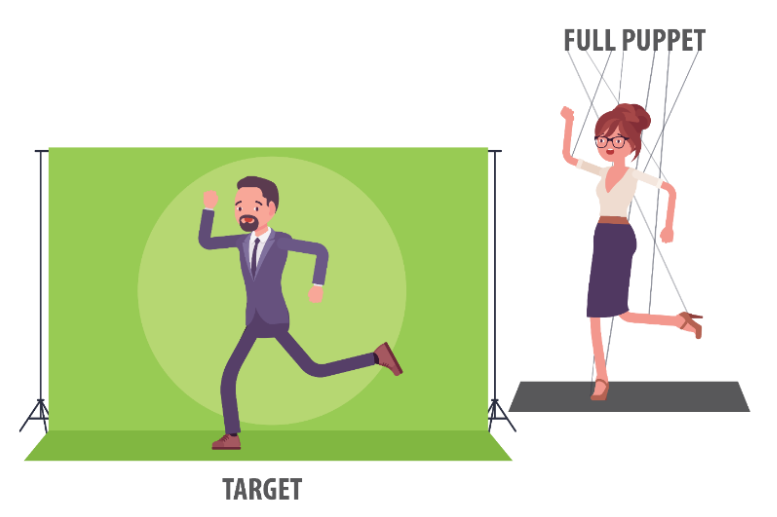
\includegraphics[width=.41\linewidth]{other-fig/full_puppet.png}
        \caption{Full puppet technique visualisation. Retrieved from~\cite{TheThreatOfDeepfakes}.}
        \label{fig:full_puppet}
    \end{figure}

    \item Morphing – It is a type of manipulation that is used to create artificial biometric face samples. Final face contains resemble biometric information of two or more individuals. It should be possible to be successfully verified by biometrics systems for all individuals who were source for given deepfake. Fig.~\ref{fig:morphing} shows an example of a morphed image.
    \begin{figure}[H]
        \centering
        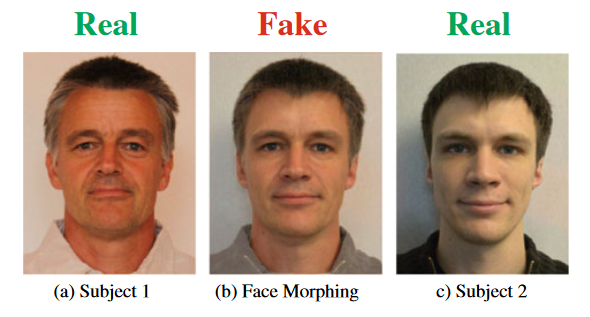
\includegraphics[width=.45\linewidth]{other-fig/morphing.png}
        \caption{Examples of fake morphed identity from Subject 1 and Subject 2. Retrieved from~\cite{IntroductionToDigitalFaceManipulation}.}
        \label{fig:morphing}
    \end{figure}

    \item Attribute manipulation – Face editing or face retouching technique involves modifying some attributes such as length or color of hair, color of skin, sex, age, adding glasses or other artefacts, and more. Fig.~\ref{fig:attribute_manipulation} shows an example of this technique.
    \begin{figure}[H]
        \centering
        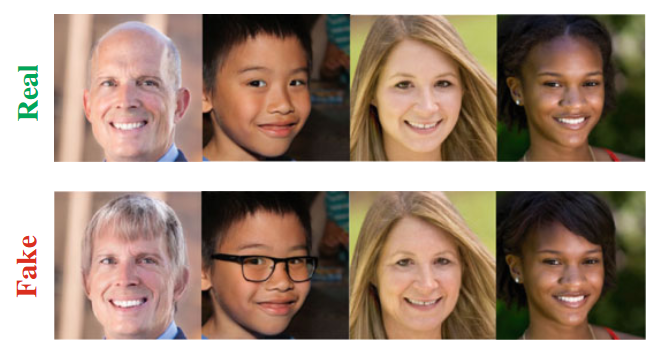
\includegraphics[width=.52\linewidth]{other-fig/attribute_manipulation.png}
        \caption{Examples of real and fake attribute manipulation category. Retrieved from~\cite{IntroductionToDigitalFaceManipulation}.}
        \label{fig:attribute_manipulation}
    \end{figure}

    \item Expression swap – Modifying facial expression of the subject as shown in fig.~\ref{fig:expression_swap}. This technique is used as one of part for full puppet.
    \begin{figure}[H]
        \centering
        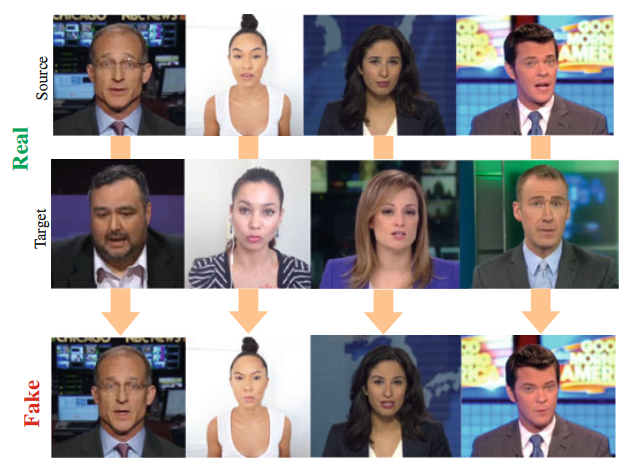
\includegraphics[width=.52\linewidth]{other-fig/expression_swap.png}
        \caption{Examples of real and fake expression swap category. Retrieved from~\cite{IntroductionToDigitalFaceManipulation}.}
        \label{fig:expression_swap}
    \end{figure}

    \item Audio/text to video – This method related to expression swap synthesising facial expression from audio or text. It is also known as lip-sync deepfakes. Diagram in fig.~\ref{fig:audio_to_video} shows how this method works.
    \begin{figure}[H]
        \centering
        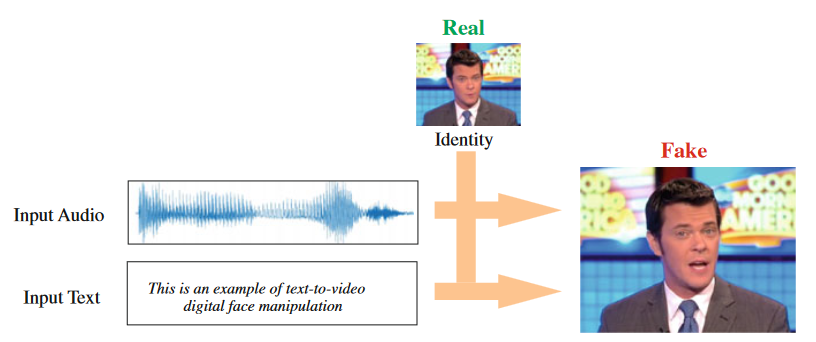
\includegraphics[width=.6\linewidth]{other-fig/audio_to_video.png}
        \caption{Examples of real and fake audio/text to video fake category. Retrieved from~\cite{IntroductionToDigitalFaceManipulation}.}
        \label{fig:audio_to_video}
    \end{figure}
\end{itemize}

Creating deepfakes nowadays is complex task and many deepfakes is using more techniques so that they could be included into more than one category. Attackers can possibly create identity swap deepfake and after that apply attribute manipulation to this deepfake to tune final results.

% ----------------------------------------------------------------------- %
\chapter{Deepfake detection}
\label{chapter:deepfake_detectoin}

As we stated, humans are not good at recognizing deepfakes. Creating deepfakes could leave visible defects (e.g., blurring or misalignment on edges in the image). A. Firc~\cite{ApplicabilityOfDeepfakes} summarizes the list of features to focus on when spotting fakes for humans.

\begin{itemize}
    \item Facial features – eyes and their movement, eyebrows, glasses, facial expression, hair and facial hair, skin, lips, teeth
    \item Body features – body position and posture, body movements
    \item Voice features – unusual tempo, end of words, fricatives, conversation
    \item General indices – blurring or misalignment on edges, inconsistence noise or audio
\end{itemize}
	
This list points to critical parts where defects, which were created during the creation of deepfake, could be spotted. Generation of deepfakes is getting better, plus other masking techniques are being used. The big problem for detection is lossless compression, several chained resizes of an image, application of noise, etc. Basically, all methods that lead to some degree of data loss, but without noticeable change for the naked eye or ear. When generation of deepfakes is not good enough manual post-processing could be used for polishing results (images – Photoshop, GIMP, etc.). 

Machine detection could be divided into two categories: standard algorithms looking for physical inconsistency and digital integrity, using the same features as Firc described. Other methods are based on machine learning. The same “masking” techniques listed before (compression, chained resizes, etc.) have the same effect on machine-based detection. Any data loss prevents the usage of reliable methods such as frequency analysis. Still, computers perform better than humans because they can also use different features (e.g., pixel-level features), especially neural networks trained for deepfake detection.~\cite{MediaForensicsandDeepFakes}

The problem of neural networks is that we do not know what it is learnt to detect. It depends highly on training dataset. Probably the worst case scenario would be only recognizing suspicious images containing traces after “masking” techniques such as double compression, noise patterns, etc.

Another problem of detection algorithms is bad generalization. Most of methods are trained on single domain deepfake (e.g., identity swap), which means they are not able to recognize deepfake from different category. When methods are trained on multi-domain datasets, accuracy is going down.~\cite{FacialRetouchingAndAlterationDetection}

\section{Image/Video detection methods}

As stated, before most of methods for deepfake detection are targeting only single domain. This section will describe examples of proposed detection methods for image/video deepfakes. There are more conventional approaches and also more “exotic”.

P. Majumdar, et al. referring to multiple detection methods for image retouching (makeup, filters) and alternation (fully synthetize faces, morphing)~\cite{FacialRetouchingAndAlterationDetection}. Most of them use the same pattern which could be described as specific feature extraction followed by support vector machines (SVM) for classification. One of the methods proposed detection of images using face patches as input in the deep Boltzmann machine for feature extraction and SVM for binary classification. Another method uses softmax probabilities as features for the SVM. Other methods, for example, using convolutional neural networks.~\cite{FacialRetouchingAndAlterationDetection}

L. Spreeiwers, et al. made research on using local binary pattern with SVM for morphing detection~\cite{PracticalEvaluationOfFaceMorphingAttackDetectionMethods}. A single LBP histogram contains 59 feature values, which means that for a 3 × 3 layout, the feature space has 531 dimensions. The SVM classifiers are trained on between 650 and 1,000 samples. They also stated that EER increases to above 20 \% while adding Gaussian noise to the deepfakes images.

Non-conventional detection method is heart rate estimation (remote photoplethysmography) by J. Fierret~\cite{DetectionBasedOnHeartRateEstimation}. They are trying to estimate heart rate from video and evaluating frame-by-frame. There are other human physiological processes that could for be used instead heart rate such as blood oxygen or breath rate. The score oscillates during the video and final decision is based on the mean/median/QCD score.

There are many other methods, and each will have its pros and cons, but as we can observe, SVM classification with large range of different feature extractors. Another rising group of detectors is using CNN. There are not many researches using CNN as SVM, but results seems to be promising as we can see in researches~\cite{3DCNNArchitecturesAndAttentionMechanismsForDeepfakeDetection}~\cite{CapsuleForensicsNetworksForDeepfakeDetection}.

\section{Voice detection methods}

Voice detection complicates different languages; it is similar story to image/video deepfakes. There are face swaps, morphing, etc., and for voice there are different languages and dialects. Voice detection methods also copying trend from image/video detection methods. Support vector machines (SVM) with different feature extractors or CNNs.

Z. Almutairi and H. Elgibreen refer to multiple methods~\cite{ReviewOfModernAudioDeepfakeDetectionMethods}. One of them uses the SVM model with Random Forest to predict synthetic voices based on a feature called Short-Term Long-Term. In this research, they compared SVM with many other classifiers such as Linear Discriminant, Quadratic Discriminant, Linear SVM, weighted K-Nearest Neighbors, and SVM outperforms all of them. Other referred work uses combination of two CNN, 1-D CNN and Siamese CNN. The Siamese CNN contained two identical CNNs that were the same as the 1-D CNN, but concatenated them using a fully connected layer with a softmax output layer.~\cite{ReviewOfModernAudioDeepfakeDetectionMethods}

\section{Analysis of existing tools for detecting deepfakes}

Tools for deepfake detection are slowly getting from command line tools for experts to online tools with user-friendly interface. There are not many tools of this kind and some of them are not free to use. The following lines describe two available tools in a market.

\subsection{Deepware}

The Bosnia and Hercegovina recognize danger of deepfakes, while their parent company researched methods to develop an AI-based antivirus engine. Deepware company was founded to develop scanner for deepfake recognition.

Deepware provides REST API with web UI\footnote{\url{https://scanner.deepware.ai/}}, mobile android application. The backend of this project with pre-trained models is accessible on their GitHub as Python command line tool\footnote{\url{ https://github.com/deepware/deepfake-scanner}}.

\begin{figure}[H]
    \centering
    
\includegraphics[width=.65\linewidth]{other-fig/deepware_input.png}
    \caption{Deepware scanner input form}
    \label{fig:deepware_input}
\end{figure}

\begin{figure}[H]
    \centering
    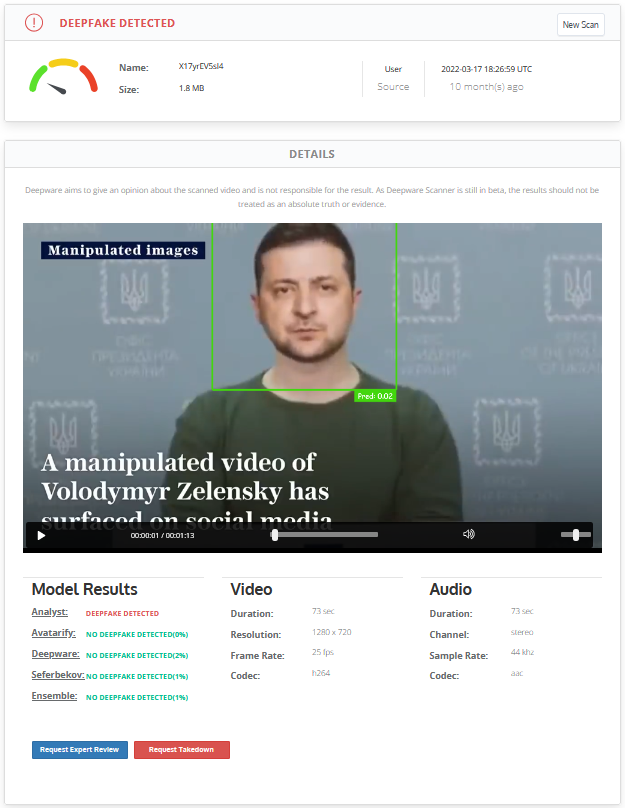
\includegraphics[width=.58\linewidth]{other-fig/deepware_results.png}
    \caption{Results of Deepware scanner containing probability of deepfakes from multiple detection methods}
    \label{fig:deepware_results}
\end{figure}

The web application is stating that the project is in Beta, but unfortunately the last commit to the GitHub repository was made on 7th of June 2022 reported at the time of writing this thesis.

The tool provides a simple user interface to scan only videos. The user can input the link to the video (e.g., YouTube) or upload the video file directly as shown in fig.~\ref{fig:deepware_input} . There are many supported video formats. The only limitation is the length of the video, which does not have to be longer than 10 minutes.

Processing of approximately 1 minute long video takes several seconds (3-10 seconds). Results contains video and audio metadata, results of multiple detection methods/models, and deciding whether it is a deepfake or not with gauge chart of confidence as we can observe in fig~\ref{fig:deepware_results}. To use their Rest API, you need to request authentication token. API provides the same functionality as web UI via three methods.

\begin{itemize}
    \item POST /video/scan
    \item GET /url/scan
    \item GET /video/report
\end{itemize}

The first two methods execute scan on a video file or link and return report ID. Results report could be retrieved by last method and results are returned as JSON. Documentation also code samples for multiple programming languages on how to use API properly. The provided API can be integrated to other processes like mail communication scans or file upload filters.

\begin{table}[H]
    \centering
    \begin{tabular}{|l|r|r|r|}
        \hline
        & \multicolumn{1}{l|}{\begin{tabular}[c]{@{}l@{}}Correct\\ (deepfake/original)\end{tabular}} & \multicolumn{1}{l|}{\begin{tabular}[c]{@{}l@{}}Incorrect\\ (deepfake/original)\end{tabular}} & \multicolumn{1}{l|}{Scan failed} \\ \hline
        Celeb DF & 10/7 & 0/0 & 3 \\ \hline
        FaceForensics++ & 4/5 & 1/0 & 10 \\ \hline
    \end{tabular}
    \caption{Deepware manual testing results}
    \label{table:deepware}
\end{table}

Deepware did not provide requested API key, so in table~\ref{table:deepware} you can find results of manual testing. The test contains 40 videos from two different deepfakes datasets (20 from CelebDF and 20 from FaceForensics++). The distribution between original and deepfakes videos was 1:1. The accuracy of detection is decent, but from 40 tested files 13 files did not go through scan, even repeatedly. It is a very small sample, so we leave it to the reader to draw conclusions.

\subsection{Sensity}

Sensity is very similar from the user perspective to Deepware. Based on the post on Sensity blog~\cite{HowToDetectADeepfakeOnline} from 2021 we can explore web UI of their application. The application is not publicly accessible and to obtain access, you need to request it. Sensity provides more tools related to cybersecurity, person identification, and verification. 

Sensity allows for detection of images and videos by inserting files or referencing them via a URL link as shown in fig.~\ref{fig:sensity_input}. Sensity allows processing of quite small group of file types (png, jpeg, jfif, tiff, mp4, mov). Another limitations are for videos regarding their size (up to 30MB), length (10 minutes), and quality of videos (1440p).~\cite{HowToDetectADeepfakeOnline}

\begin{figure}[H]
    \centering
    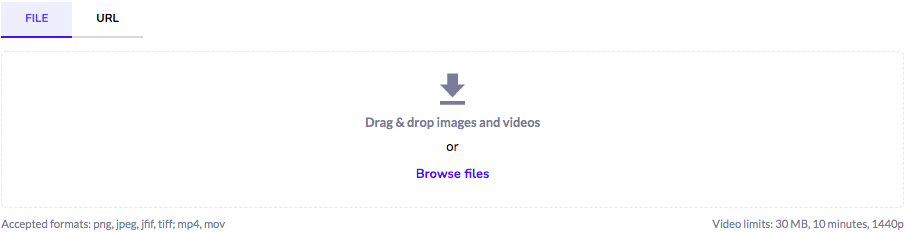
\includegraphics[width=.95\linewidth]{other-fig/sensity_input.png}
    \caption{Sensity deepfake detection tool input form. Retrieved from~\cite{HowToDetectADeepfakeOnline}.}
    \label{fig:sensity_input}
\end{figure}

The tool is capable of recognize only face swap and fully synthesized faces by GAN. It is not able to recognize morphed images or other deepfakes. For GAN-genereated faces, it is sometimes able to classify model generator. If deepfake is recognized tool show how confident he is, all shwon in fig.~\ref{fig:sensity_results}. Compared to Deepware, it provides image scans; on the other hand, it does not have mobile application.

\begin{figure}[H]
    \centering
    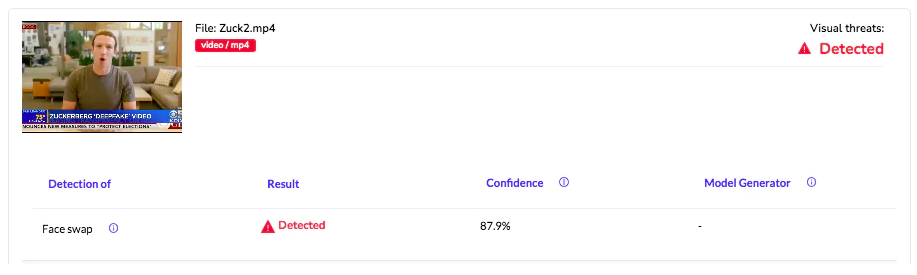
\includegraphics[width=.95\linewidth]{other-fig/sensity_results.png}
    \caption{Sensity deepfake detection tool results. Retrieved from~\cite{HowToDetectADeepfakeOnline}.}
    \label{fig:sensity_results}
\end{figure}

\subsection{Other}

Below you can find a list of other open source detection methods. These methods usually require a good knowledge of information technologies and programming to make them work on your computer. There is no guarantee that these methods really work, but two projects were selected for integration into the framework arising in this work.

\begin{itemize}
    \item Video
    \begin{itemize}
        \item dfdc\_deepfake\_challenge \\ (\url{https://github.com/selimsef/dfdc_deepfake_challenge})
        \item DeepFake Detection \\ (\url{https://github.com/dessa-oss/DeepFake-Detection})
        \item fakeVideoForensics \\ (\url{https://github.com/bbvanexttechnologies/fakeVideoForensics})
        \item Deepstar \\ (\url{https://www.zerofox.com/deepstar-open-source-toolkit/})
    \end{itemize}
\newpage
    \item Audio
    \begin{itemize}
        \item AudioDeepFakeDetection \\ (\url{https://github.com/MarkHershey/AudioDeepFakeDetection})
        \item specrnet \\ (\url{https://github.com/piotrkawa/specrnet})
    \end{itemize}
\end{itemize}

% ----------------------------------------------------------------------- %
\chapter{Architecture and technologies analysis}

The goal of this work is to develop a deepfake detection framework capable of serving various client applications and an exemplary web plugin that communicates with framework and clearly displays the results to the user. We already analyze the market and test existing tools. Because there is no external contracting party defining their need, we will define requirements by ourselves. Requirements will be divided into two categories, functional and non-functional requirements. It is important to define not only functional logic, but also some limits on processing time, number of users, etc.

\section{Requirements}

As we already said, the framework has to support multiple different types of clients (e.g., mobile, web), so there needs to be a properly defined communication interface between the client applications and the framework itself, which will act as server in this case. Framework allows dynamic changing detection methods, which means it is able to add, remove, or edit detection method. This implicates multiple detection methods at one time for image, video, and voice. Editing detection method means updating the model or constant parameters. 

The platform should support as many file types as possible and adding a new method should not affect methods already presented in the framework, within supported file types. Different detection methods have different models depending on their design, so model management will be wrapped completely into the detection method.

The framework should collect statistics and hardware metrics, but the collection of personal information should be omitted. All collected metrics will be used for future improvements of detection methods and optimizing operating costs and performance. We would like to have a short response time with as low operating costs as possible. Those two parameters are in contradiction, so there has to be some balance between them. 

Different cloud services offer their own tools for collecting metrics, but our system should be operating platform independent. That means framework needs to be consist of application, which collects metrics and provides them to other parts of framework, or person who operates the framework.

From a number of users perspective, the platform will handle up to hundreds of users at one time, and with enough resources the framework should handle even more. Scalability of computationally intensive parts of the framework will help meet these requirements. 

The client application has to be simple so that anyone can use it. Users should be able to upload files or put a link to a file. The web plugin allows access to DOM of the webpage so an optional extension for client application will be selection of web element for detection. Application then retrieve metadata from selected element automatically. 

Working with provided links or elements on specific pages brings several complications such as authentication. The framework does not have user context, so he is not able to retrieve all data that user has access to. We will not deal with these issues and if the file cannot be access, the processing request will not be created. It will be one of possible future improvements to the framework.

Because it should cover a large group of possible users, results have to be easy to understand and also provides information for experienced users. Last but not least, the client application should enable users to send feedback.

There are several web browsers in market that cover almost all audience, so the developed web plugin should be portable among multiple web browsers. Today it is standard, but it is necessary to mention that the application should be secured. It will affect code of framework, client application, and environment itself (hardware, operating systems, …). All work is open-source and accessible on the public GitHub repository\footnote{\url{https://github.com/PlayerBerny12/VUT-DIP-Code}}.
\\\\
\noindent Summary of functional requirements:
\begin{itemize}
    \item Adding, removing, and editing (changing parameters and models) detection methods
    \item Multiple detection methods at once
    \item Collecting statistics and feedback
    \item Detection of image, video, and voice
    \item Detection of file, URL link, or selected HTML element (optional)
    \item Understandable presentation of results
    \item Security
\end{itemize}

\noindent Summary of non-functional requirements:
\begin{itemize}
    \item Scalability
    \item Small response time
    \item Low operating costs
    \item Portability of the web plugin among multiple web browsers (optional)
    \item Open source
\end{itemize}

\section{Containerazation}

The framework requires dynamic management of the detection methods. It means that the framework can contain one or twenty different detection methods. Each method could be developed using different programming languages or technologies. Model management will be encapsulated and handled by each detection method individualy. This leads to some isolation of methods with a well defined communication protocol. 

Scalability of framework, isolation and resource management, all this together will be reached via containerization. There are many technologies dealing with containers, such as Docker, Podman, LXC. When we start counting orchestration with automatic scalability, the number of technologies drops down.

Azure and AWS offer their own container orchestrators: Azure Container Instances~\cite{AzureOrchestrators}, Amazon Elastic Container Service~\cite{AWSOrchestrators}. As already stated, the framework should be operating platform independent, so looking only for orchestrator supported by all cloud providers, we discover Kubernetes. Google Cloud, AWS and Azure support Kuberentes, and no other alternative supported by all of them exist.~\cite{AzureOrchestrators}~\cite{AWSOrchestrators}~\cite{GoogleOrchestrators}

Docker is probably the most widely used technology for containerization. Podman is another containerization technology having similar API to Docker. Podman is newer and has different architecture than Docker which results in a more secure operation and fewer resources required for running~\cite{DockerPodman}. But still, we will stick with duo Kubernetes and Docker because of the huge community and good support of Docker in Kubernetes and also less concerns about possible issues during development.

\section{Framework}

The framework is a collection of detection methods, an interface for the client application (receiving requests, sending report response), and orchestrates/arranges all communication. It will be built into several containers and one of the containers will be providing client application interface. It could be Rest API~\cite{RestAPI}, GraphQL~\cite{GraphQL} or custom protocol. It is not a good idea to develop a custom communication protocol, and because of simplicity of interface we will use the most used one, Rest API. For this purpose, we can use a huge number of different technologies such as ASP.NET Core, Flusk, Django, Ruby on Rails, etc. Basically all named technologies meet defined requirements (response time, number of users, ect.) because most of them are covered by microservice design and they are able to run in containers. Our choice is ASP.NET Core because it has a huge community, Linux support, many external libraries, open-source development, it is suitable for bigger projects, and it has good speed of program development~\cite{ASPNETCore}.

Communication among containers will be through message broker. There are several alternatives such as Memphis, RabbitMQ, or Apache Kafka. All of them are open source and possibly suitable for our use case. The final choice is RabbitMQ because of small resource consumption, a quite large community, and this project is developed since 2007. That means we can count on future development and updates.~\cite{MessageBrokers}

The framework also needs an application for collecting metrics. Here, we chose Prome\-theus~\cite{Prometheus} and Grafana~\cite{Grafana}. Both tools are free to use and open source. Prometheus is collecting metrics, but it is not a good visualization tool; for this purpose, there will be Grafana. Grafana provides dashboards where all metrics could be presented as graphs, etc. Reasons why we take Prometheus and Grafana is because they have good cooperation and RabbitMQ has metrics compatible with Prometheus~\cite{RabbitMQMonitoring}. Capturing resources is performed by Node Exporter. It is another open source project from Prometheus, which ensures good compatibility with the previously mentioned systems~\cite{NodeExporter}.

All previously selected technologies also have good support of Kubernetes and in some cases provide custom Kuberetes operators for easier deployment. More details about it are provided in chapter~\ref{chapter:framework_implementation}.

\section{Web browser plugin}

Web plugins are based on web technologies such as HTML, CSS, JavaScript, TypeScript, etc. Because of portability and good integration, we will choose HTML, CSS, and Typescript. Typescript is a strict syntactical superset of JavaScript and adds optional static typing to the language. It is also compiled into JavaScript~\cite{Typescript}.

There are several Typescript frameworks that speed up development of application and make portability among different browsers easier. Angular seems to be as good viable option and it is frontend framework, with which we have most experience~\cite{Angular}.

Browser extensions are integrated through a standard called “Web app manifest”. It is the definition of manifest file used for integration extensions to browser, now in version~3. Standard defines the structure of the manifest that allows the configuration of different types of capabilities.  All browsers have partial or full support. Using this manifest should help to integrate the extension with browsers such as Google Chrome, Microsoft Edge, or Mozilla Firefox.~\cite{WebAppManifest}

% ----------------------------------------------------------------------- %
\chapter{Framework architecture}

The architecture must reflect that each detection method could be developed by different technology stack. We can isolate the detection methods from each other and wrap them into independent services. We do not need communication among all methods because they do not cooperate or share any data. In this case, the microservice architecture meets all defined requirements.

\section{Microservice architecture}

Microservice architecture is the style of developing applications. Example of design can be observe in fig.~\ref{fig:microservice_architecture}. The microservice allows the application to be separated into smaller logical independent parts. The service then has its own realm of responsibility and they can communicate with each other. The use of containers for the deployment of microservice application is a well-suited option.~\cite{WhatIsMicroservicesArchitecture}

\begin{figure}[H]
    \centering
    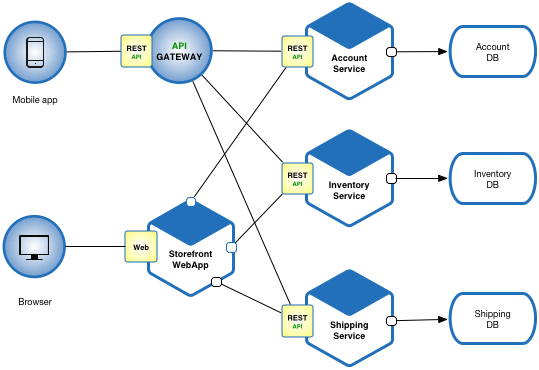
\includegraphics[width=.7\linewidth]{other-fig/microservice_architecture.png}
    \caption{Microservice architecture of fictitious e-commerce application}
    \label{fig:microservice_architecture}
\end{figure}

Microservices improve fault isolation that non-functional service should not affect others, in best case scenario. For example, if one service contains a memory leak, it is not propagated into other ones. In real cases microservices depend on each other and this might lead to a problem. Another benefit was already mentioned, and it eliminates commitment to one technology stack. One service has better maintainability because it should be small (better understandability, faster tools, etc.), which leads to more productive development.

This architecture also has several drawbacks. It increases the complexity of the architectural design and the additional implementation of cross-service communication. Here comes the usage of message brokers. When saving data to the database, there are several approaches on how this could be implemented. You do not want your database to be bottleneck of your system, so developers in most cases have to deal with distributed database systems.~\cite{MicroserviceArchitecture}

\section{High-level architecture}

The client application communicates directly with the Rest API endpoint. It is responsible for handling requests, preparing and validating data, and selecting which type of processing should be used. After processing is done, it collects all results, stores them in database, and distributes them back to the client application. Fig.~\ref{fig:framework_architecture} contains high-level design of a framework with data flow. Numbers represent steps in which order data flow through the framework.

\begin{figure}[H]
    \centering
    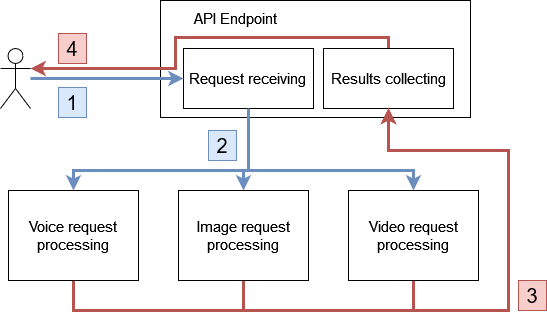
\includegraphics[width=.7\linewidth]{other-fig/framework_architecture.png}
    \caption{High-level design of whole framework}
    \label{fig:framework_architecture}
\end{figure}

The architecture separates voice, image, and video detection into an independent units. Each unit contains a processing queue where the request will be assigned by the API endpoint. The queue is serviced by one or multiple processing units that contain all related detection methods as shown in fig.~\ref{fig:framework_architecture_request_processing}.

\begin{figure}[H]
    \centering
    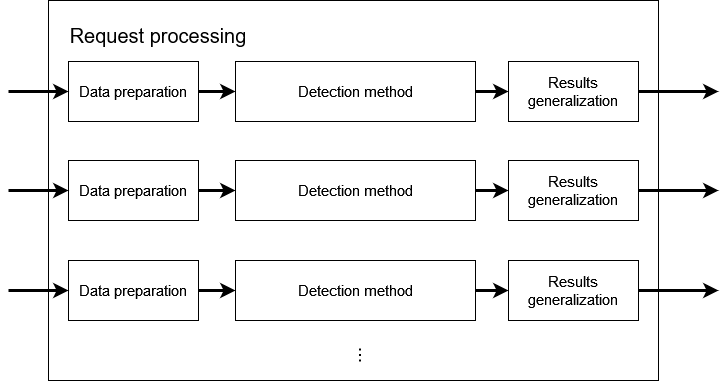
\includegraphics[width=.65\linewidth]{other-fig/framework_architecture_request_processing.png}
    \caption{Request processing detail}
    \label{fig:framework_architecture_request_processing}
\end{figure}

The processing unit works as a parallel pipeline. Closer look at design is in fig.~\ref{fig:framework_architecture_processing_unit}. Some detection methods require input data in specific format, others not, so the first step is optional data preparation. The next step is the detection method that decides whether the input data contains deepfake. Detection methods are different, so are their results. As last step it is need to properly generalize and also normalize resulting values to interval from 0 to 1.

\begin{figure}[H]
    \centering
    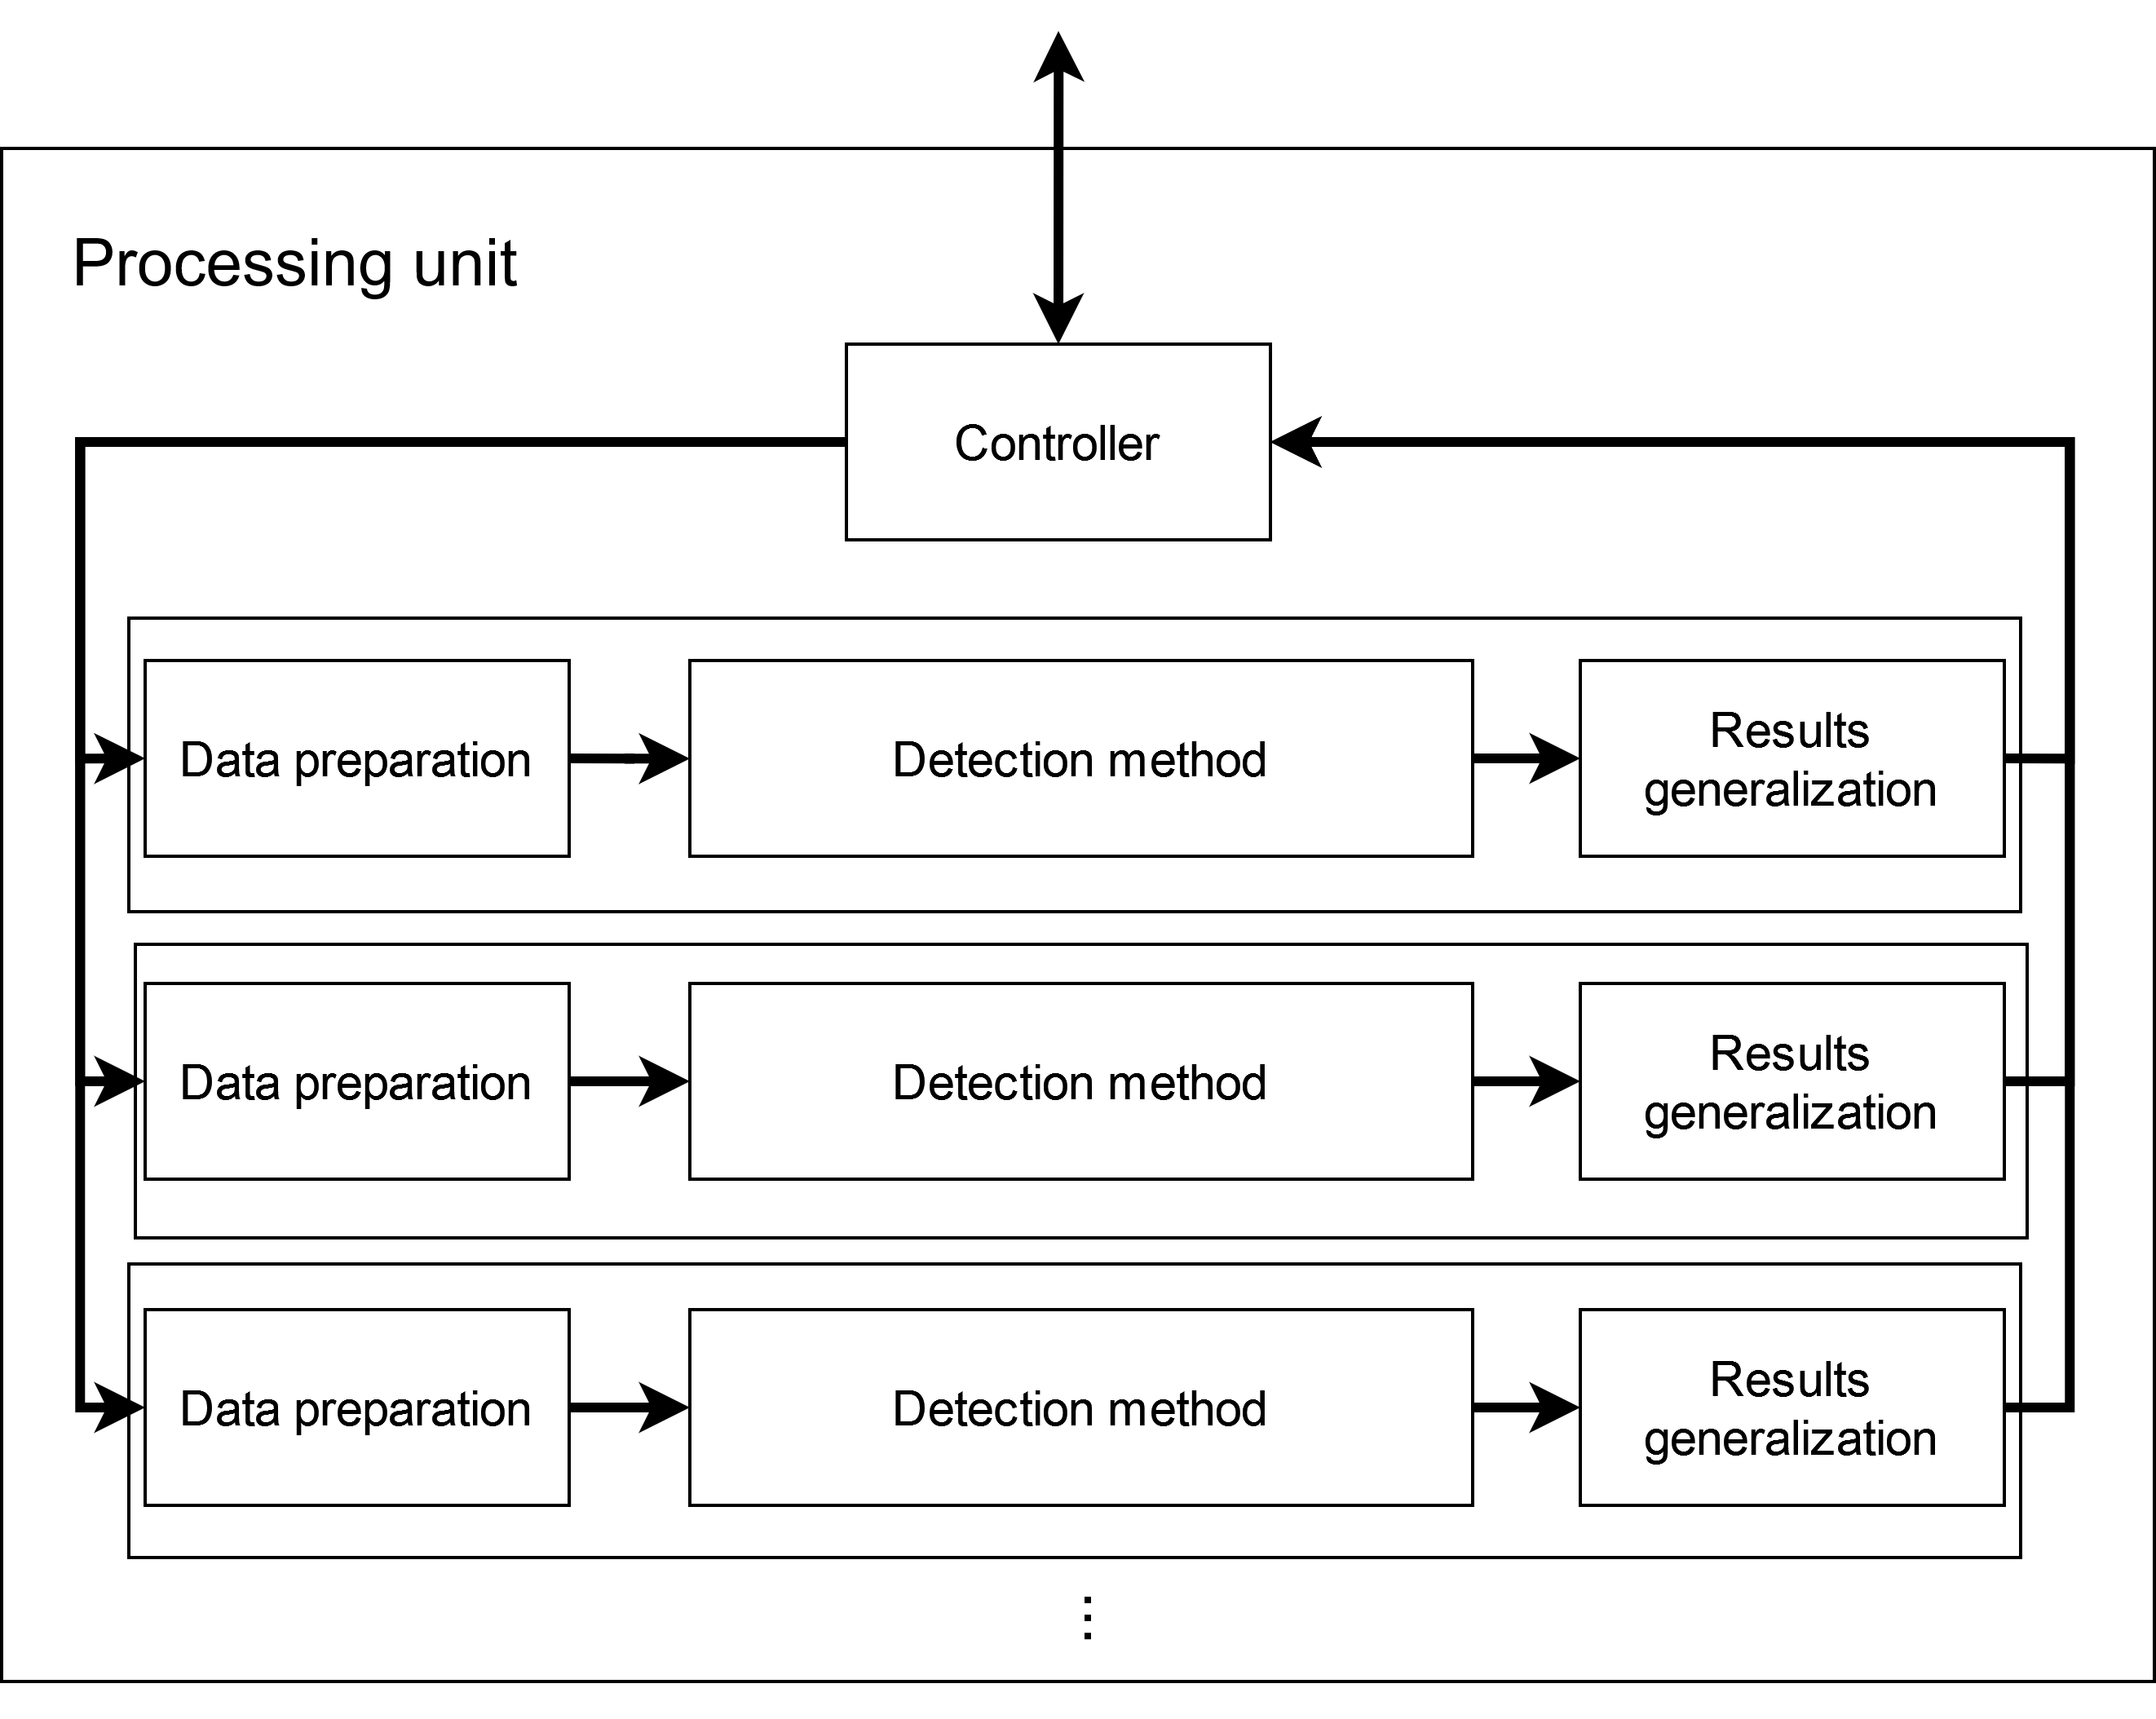
\includegraphics[width=.65\linewidth]{other-fig/framework_architecture_processing_unit.png}
    \caption{Processing unit pipeline}
    \label{fig:framework_architecture_processing_unit}
\end{figure}

\section{API Endpoint}

As mentioned before, API endpoints communicate directly with client application and with backend processing mechanism. Processing takes some time, so client application creates request and wait asynchronously to be processed by the framework. The API for this purpose contains \texttt{detect} and \texttt{request} methods.

\texttt{Detect} methods calculates checksum of file and lookup in database if there is request with same file checksum. If any request is found, then new request is not created and found request is returned. In case there is no request with same checksum new request is created and stored in database. Then this request is move into next step of processing. 

There are other support methods for health check or providing feedback. All methods are described in following list:

\begin{itemize}
    \item /ping
    \begin{itemize}
        \item GET /ping – healtcheck endpoint
    \end{itemize}
    \item /detect
    \begin{itemize}
        \item POST /detect/file – creates request with file in HTTP request body
        \item POST /detect/link – creates request with link to file in HTTP request query parameters
    \end{itemize}
    \item /request
    \begin{itemize}
        \item GET /request/results/ – returns results of processed request or empty results if request is in process
    \end{itemize}
    \item /feedback
    \begin{itemize}
        \item POST /feedback/<request\_id> - collects user feedback with optional parameter request\_id
    \end{itemize}
\end{itemize}

Each detection method has different processing times. There are two options to return results to user: partial results from the methods already completed or returns only when everything is completed. Because there is no need to show partial results, the second option will be used. The framework also calculates the overall score and this requires all results from all methods. However should not be much code changes if in future there will be need of partial results. Calculating the total score requires considering method deifferences as well as their domain focus. A single detection method is usually developed to detect only single domain (e.g., face swap). We leave the exact definition of calculation to the implementation.

The method \texttt{request/results} could be possibly replaced by websockets which will increase complexity, but on the other hand a client application could report status of the running process more precisly. It is another possible extensions to the framework.

\section{Database}

The Endpoint API needs to store some data in a database to efficiently manage multiple requests. It is also not welcome to process the same file repeatedly. By keeping the results in the database, it will save computational resources and the application will have minimal processing time for already processed files. It is also necessary to store the sent feedbacks. In fig.~\ref{fig:framework_architecture_database}, you can see the ER model of the database for this framework.

\begin{figure}[H]
    \centering
    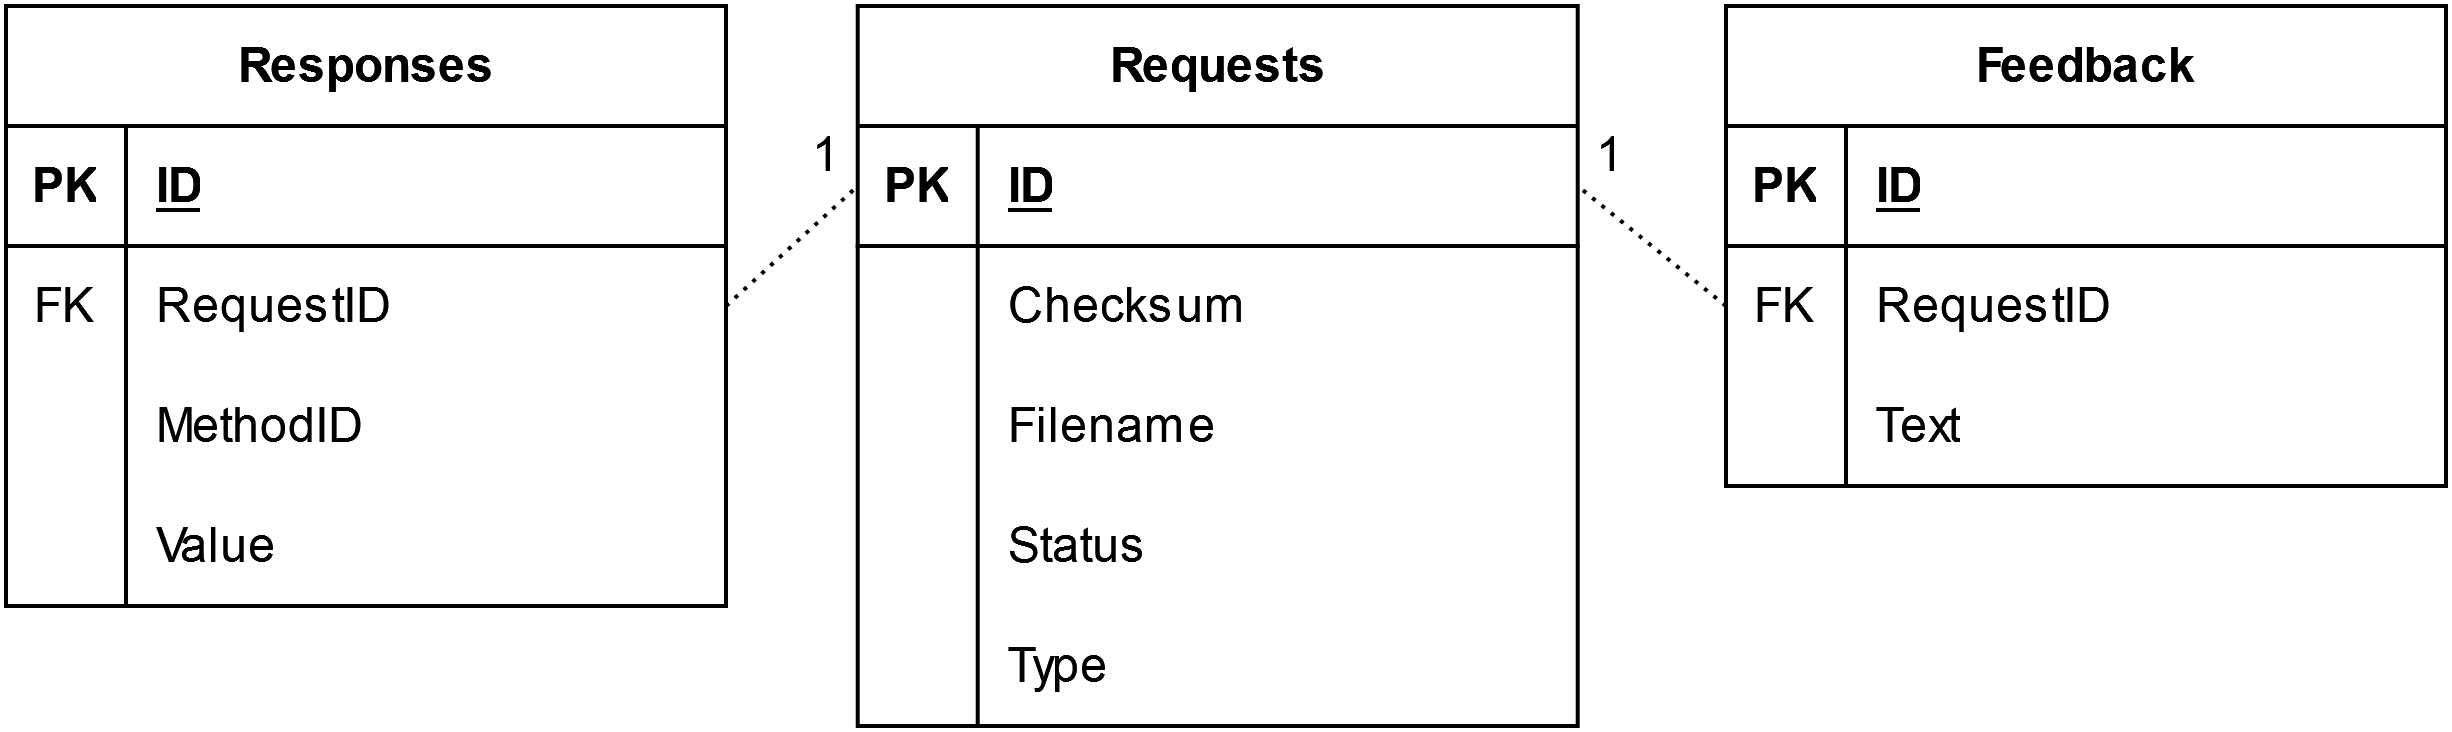
\includegraphics[width=.725\linewidth]{other-fig/framework_architecture_database.png}
    \caption{Entity-relationship model}
    \label{fig:framework_architecture_database}
\end{figure}

When any method is added or anyhow changed (e.g., different model) related or all results in database should be deleted. If we do not delete stored results users will be getting old results, that is not what we want.

\section{Request processing and processing unit}

API endpoint placing all new requests in the request queue. One of the available processing units takes the first request form queue. This request contains all the information such request ID, data for detection. Message queue in RabbitMQ will be used for this purpose.

The free controller takes the message from the queue and distributes it to all detection methods under his administration. Because each detection method is encapsulated into its own container, it needs communication channel to controller. To make integration of new detection method easy as possible we use REST API once again. The detection method should expose one method called \texttt{detect} on any port that will be placed in the controller configuration. The controller can call this method to pass parameters and start processing.

The first step in the processing pipeline is optional data preparation. The detection method could be trained only on a specific resolution of the video/image or on a specific length of the voice sample. This means that a data processing unit must be designed for a given detection method. Prepared data then are picked up by detection method and evaluated.

After detection, there is optional data generalization/normalization. Because the results must be correctly presented to user and the framework must calculate over all scores, all results need to be normalized to same interval from 0 to 1. Where zero means detected file contains deepfake and one means opposite. When results contain more specific information, in this case, they need to be generalized. The results are then pushed to the output queue.

\section{Monitoring}

One of the requirements was to collect metrics on resource consumption and also metrics on which to scale the number of processing units. Node exporter was selected as the tool to collect resource consumption metrics to be run on every node in the cluster. RabbitMQ handles the collection of metrics itself, no additional configuration is required.

Prometheus collects metrics from both of these sources and stores them in its database. Node exporter collects metrics about CPU utilization, RAM consumption, disk utilization, network card utilization, etc. RabbitMQ collects metrics about the number of messages in each queue, number of connections and channels, etc. These metrics will be displayed by Grafana in their dashboards and Prometheus will be used as a source.

\section{Containerization and scaling}

Detection methods have to be containerized, and supported methods relevant to detection are encapsulated together with detection method. Processing unit is consists of controller and multiple detection methods and all togeather it is creating multicontainer pod.

Scaling can be done vertically or horizontally. Vertical scaling changes the number of resources, such as CPU cores or the size of RAM. Horizontal scaling changes the number of nodes/units/containers that process a given task. Fig.~\ref{fig:scaling} shows the difference. Kubernetes allows automatic scaling based on the consumed resources. We use horizontal automatic scaling based on consumed resources for the number of nodes in the cluster. Second scaling uses the number of messages in the queue, and if the number of requests in the queue changes up or down, then horizontal scaling adds or reduces the number of processing units for given queue.~\cite{Scaling}

\begin{figure}[H]
    \centering
    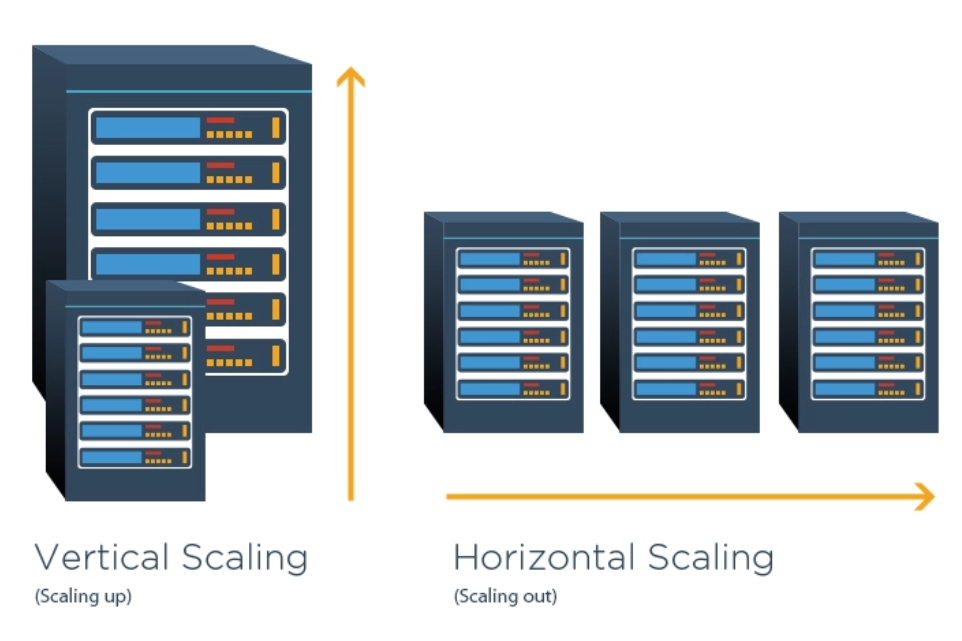
\includegraphics[width=.675\linewidth]{other-fig/scaling.png}
    \caption{Vertical and horizontal scaling comparison. Retrieved from~\cite{Scaling}.}
    \label{fig:scaling}
\end{figure}

The number of messages in queue can be found in Prometheus, but we need to make it available to the Kubernetes API. To do this we will use the Prometheus adapter; this is a project that maps defined metrics from Prometheus to messages understood by the Kubernetes API~\cite{PrometheusAdapter}. Then we just need to configure the Horizontal Pod Autoscaler to turn scaling on with usage of these values. Horizontal Pod Autoscaler will scale up when there are a lot of requests waiting to be processed in the queue. On the other hand, to save costs, it will automatically scale down when the peek of requests drops down.

% ----------------------------------------------------------------------- %
\chapter{Client architecture}

The use case of the client application is straightforward, so there is no need for use case or data flow diagrams. The application will try to prepare the file for inspection and send it to the server framework. The next section contains several wireframes of how the client application should look like with description.

\section{Web browser plugin}

It should allow the user to insert a file via file upload, link, or HTML element containing a targeted file. In fig.~\ref{fig:client_wireframe_input_selection} we can see selection of insertion types, for file upload the user will be prompted by system file upload picker. When user pick link as input, floating windows will pop up, and user then can insert URL to file. Those two selections are the same as other tools in market also provide. Optional improvement will be element selection which switches the application to interactive mode where user can point to HTML element and application will try to retrieve metadata of image or video directly from HTML. 

\begin{figure}[H]
    \begin{subfigure}[h]{.498\linewidth}
        \centering
        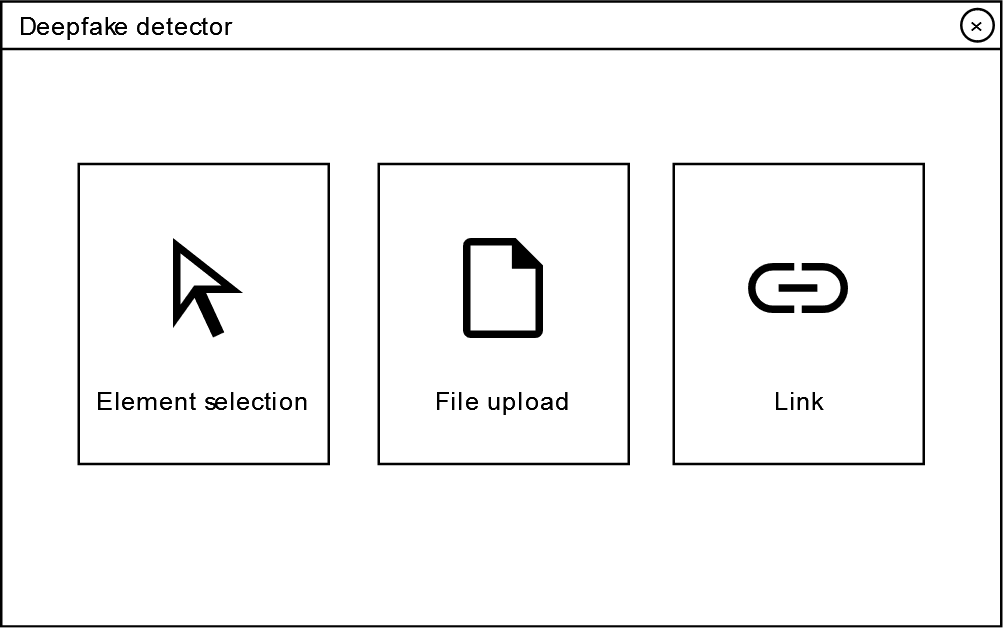
\includegraphics[width=1\linewidth]{other-fig/client_wireframe_input_selection.png}
        \caption{Input type selection}
    \end{subfigure}
    \hfill
    \begin{subfigure}[h]{.498\linewidth}
        \centering
        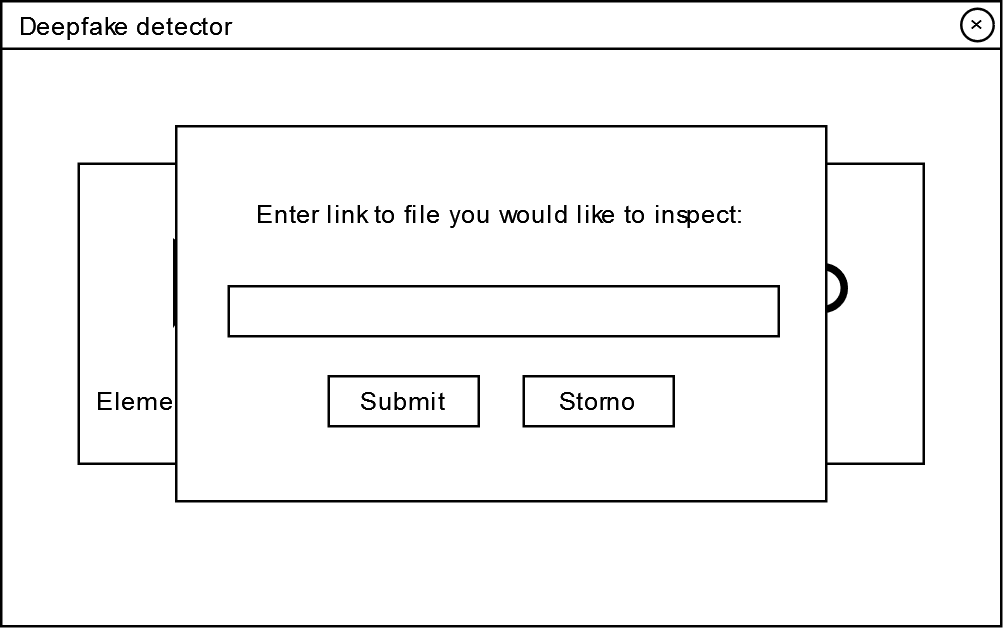
\includegraphics[width=1\linewidth]{other-fig/client_wireframe_input_selection2.png}
        \caption{Link input in floating window}
    \end{subfigure}
    \caption{Input type selection screens}
    \label{fig:client_wireframe_input_selection}
\end{figure}

Because detection framework will contain several detections method we need to show the result of each method independently. It could be a little confusing for user so there will also be overall score which interprets/generalizes all the result of each method. The overall score will indicate the results as a percentage and as emoticon. The palette will contain four emoticons shown in fig~\ref{fig:client_wireframe_results3}. For better understanding there are question marks in the UI that after mouse hover shows tooltip with description. Whole results screen can be view in fig.~\ref{fig:client_wireframe_results}.

\begin{figure}[H]
    \begin{subfigure}[h]{.498\linewidth}
        \centering
        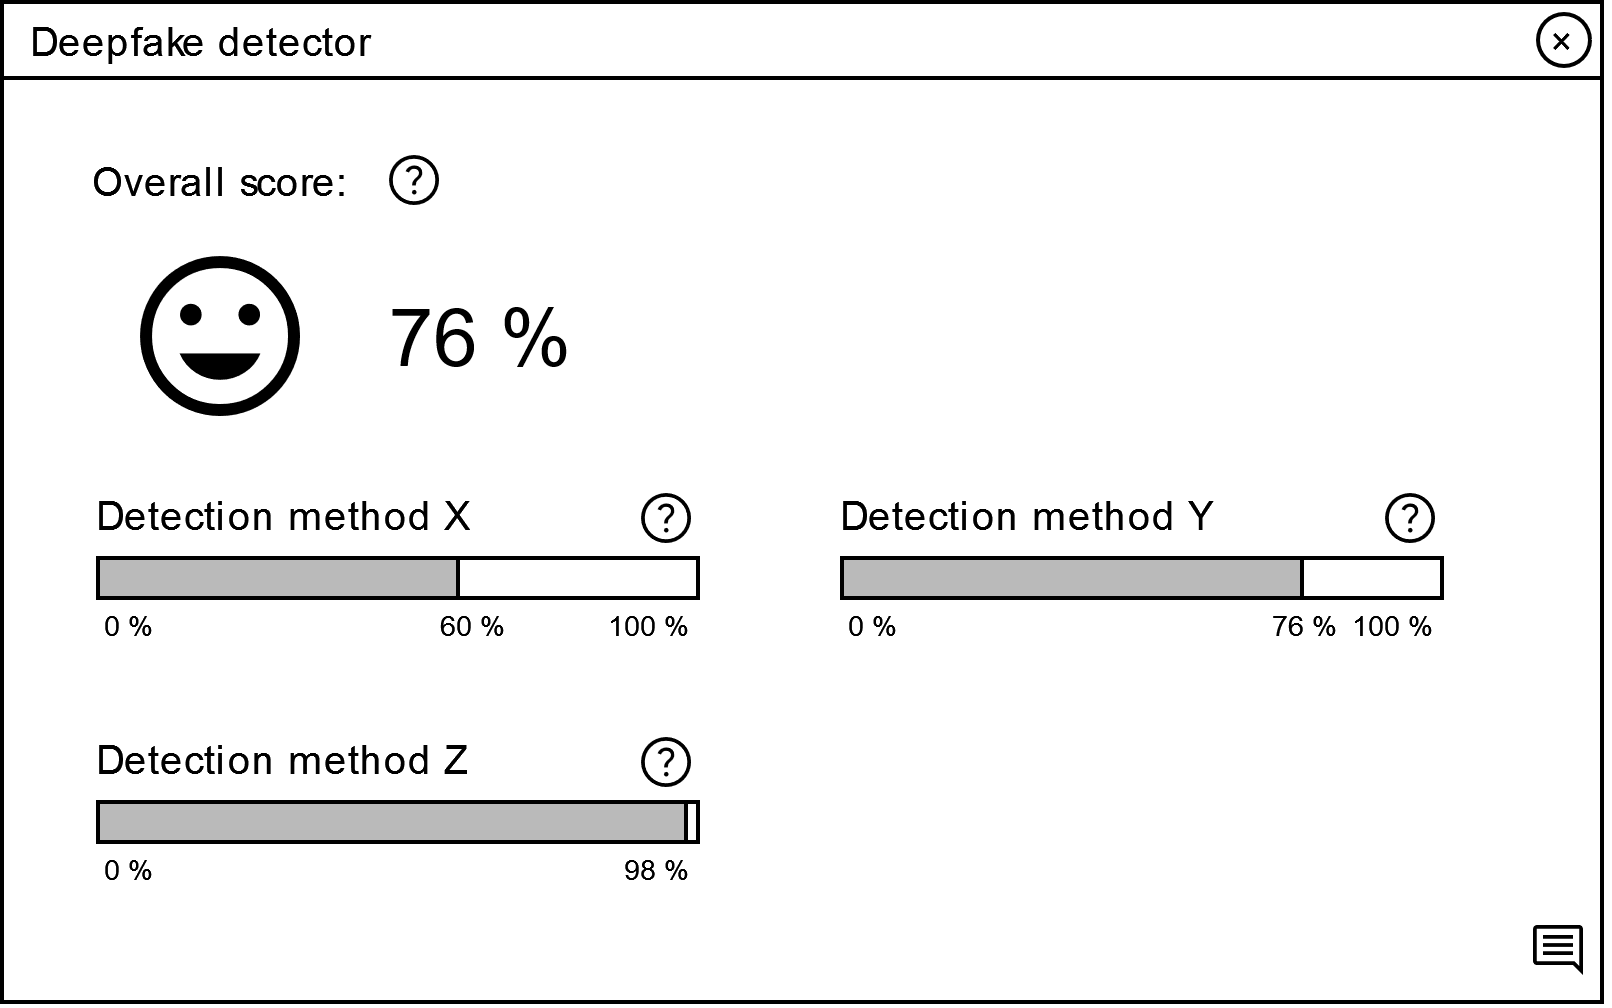
\includegraphics[width=1\linewidth]{other-fig/client_wireframe_results.png}
        \caption{Results view}
    \end{subfigure}
    \hfill
    \begin{subfigure}[h]{.498\linewidth}
        \centering
        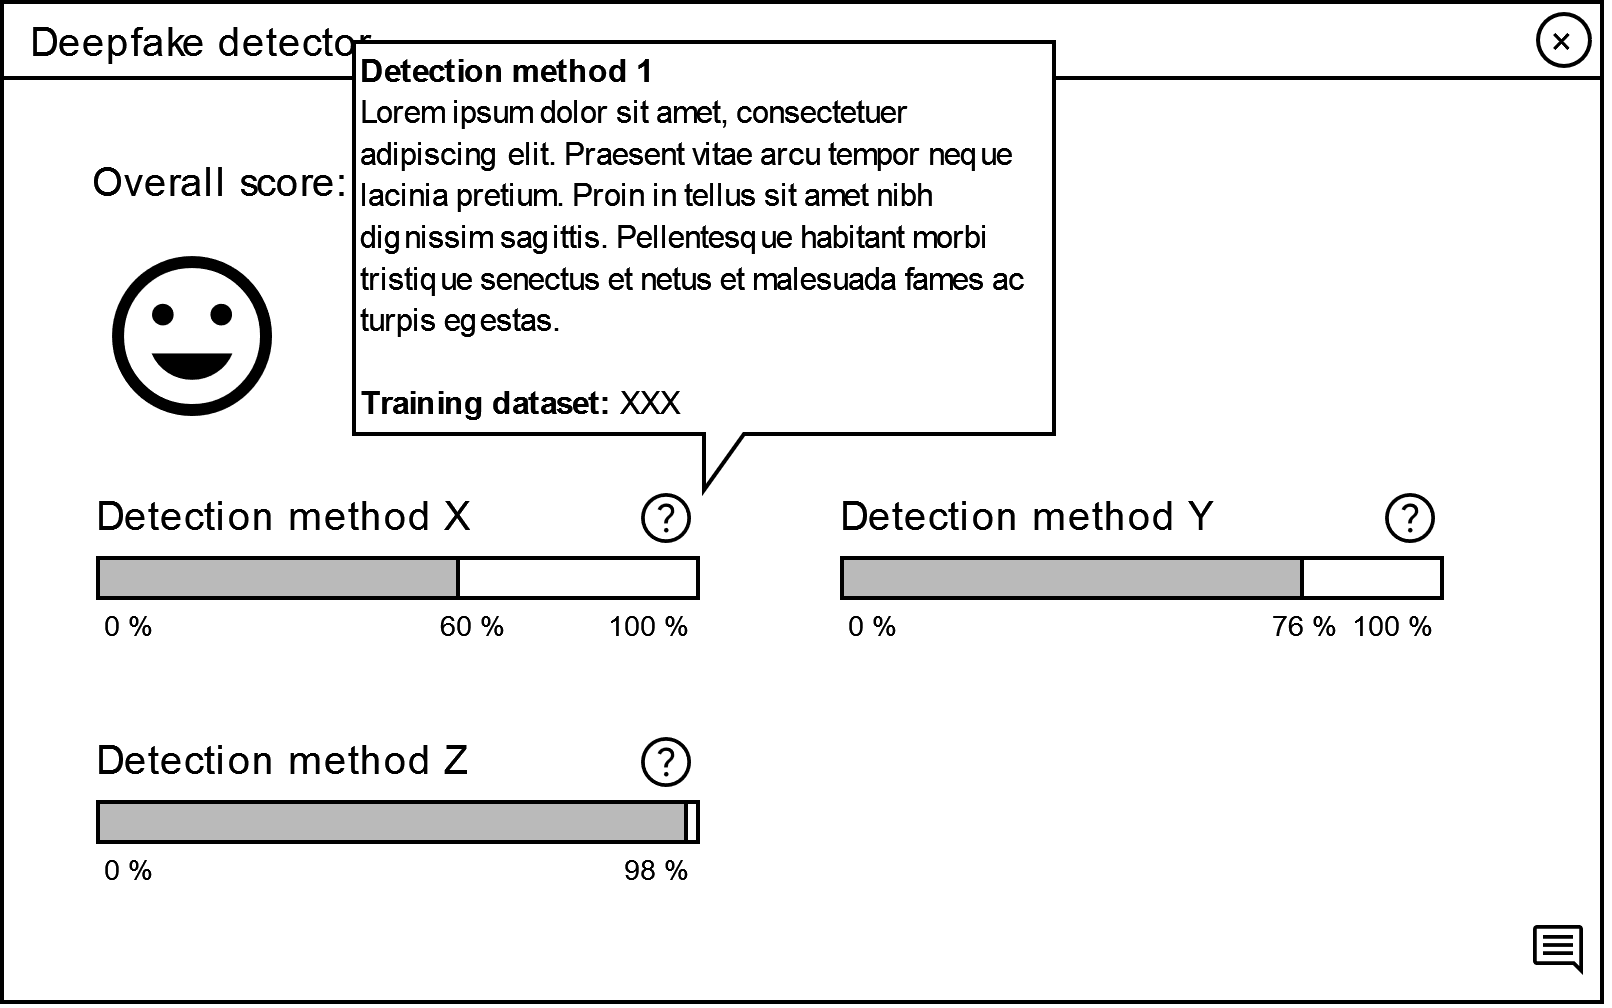
\includegraphics[width=1\linewidth]{other-fig/client_wireframe_results2.png}
        \caption{Tooltip with description of detection method}
    \end{subfigure} 
    \caption{Results view screens}
    \label{fig:client_wireframe_results}
\end{figure}

\begin{figure}[H]
    \centering
    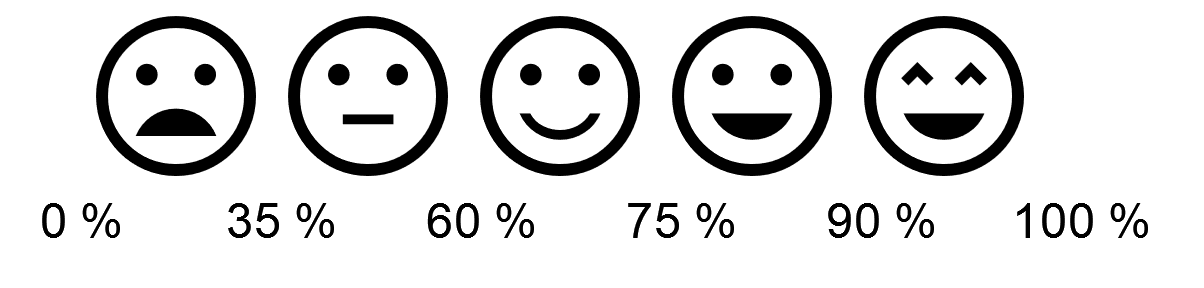
\includegraphics[width=.5\linewidth]{other-fig/client_wireframe_results3.png}
    \caption{Palette of emoticons indicating if inspected file contains deepfake or not}
    \label{fig:client_wireframe_results3}
\end{figure}

At the bottom of each screen there is an icon that enables the user to the send feedback from application. After clicking on this icon floating window will appear, shown in fig~\ref{fig:client_wireframe_feedback}. When user will be sending feedback on the result page, the internal result ID will be added as an additional parameter to the feedback message. 

\begin{figure}[H]
    \centering  
    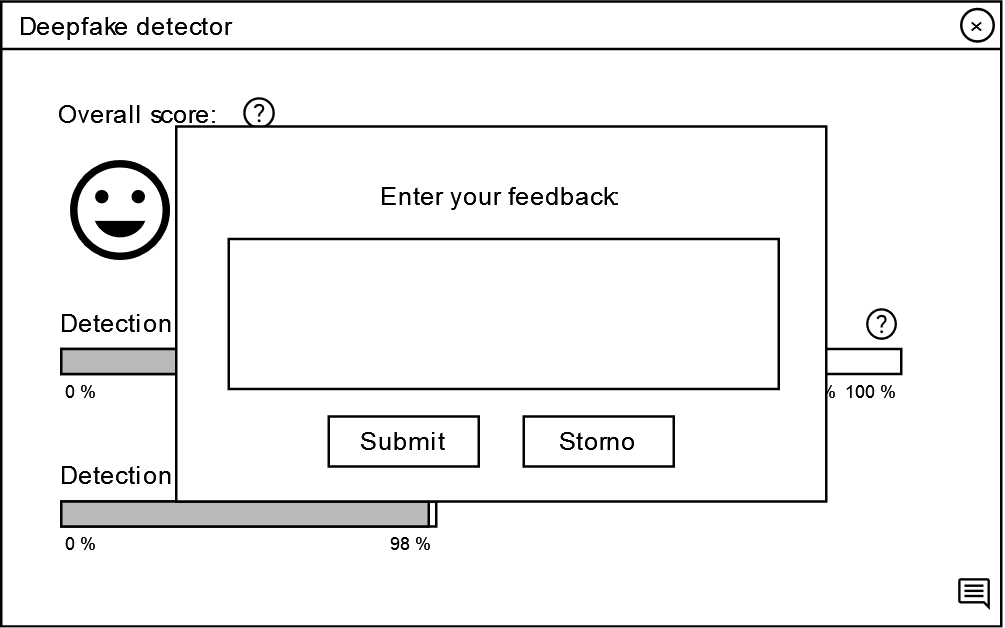
\includegraphics[width=.498\linewidth]{other-fig/client_wireframe_feedback.png}
    \caption{Feedback form in floating window}
    \label{fig:client_wireframe_feedback}
\end{figure}

% ----------------------------------------------------------------------- %
\chapter{Framework implementation and deployment}
\label{chapter:framework_implementation}

The implementation is available in the public repository\footnote{\url{https://github.com/PlayerBerny12/VUT-DIP-Code}}. The project is divided into three folders: \texttt{clients}, \texttt{server}, and \texttt{templates}. The clients folder is intended for various implementations of client applications such as web client, web browser extension, etc. Currently, only one client is implemented, but other types can be added in the future. The \texttt{server} folder contains the framework implementation and the Kuberentes deployment manifest files. The last folder contains templates for easy integration of detection methods.

\begin{figure}[H]
    \centering
    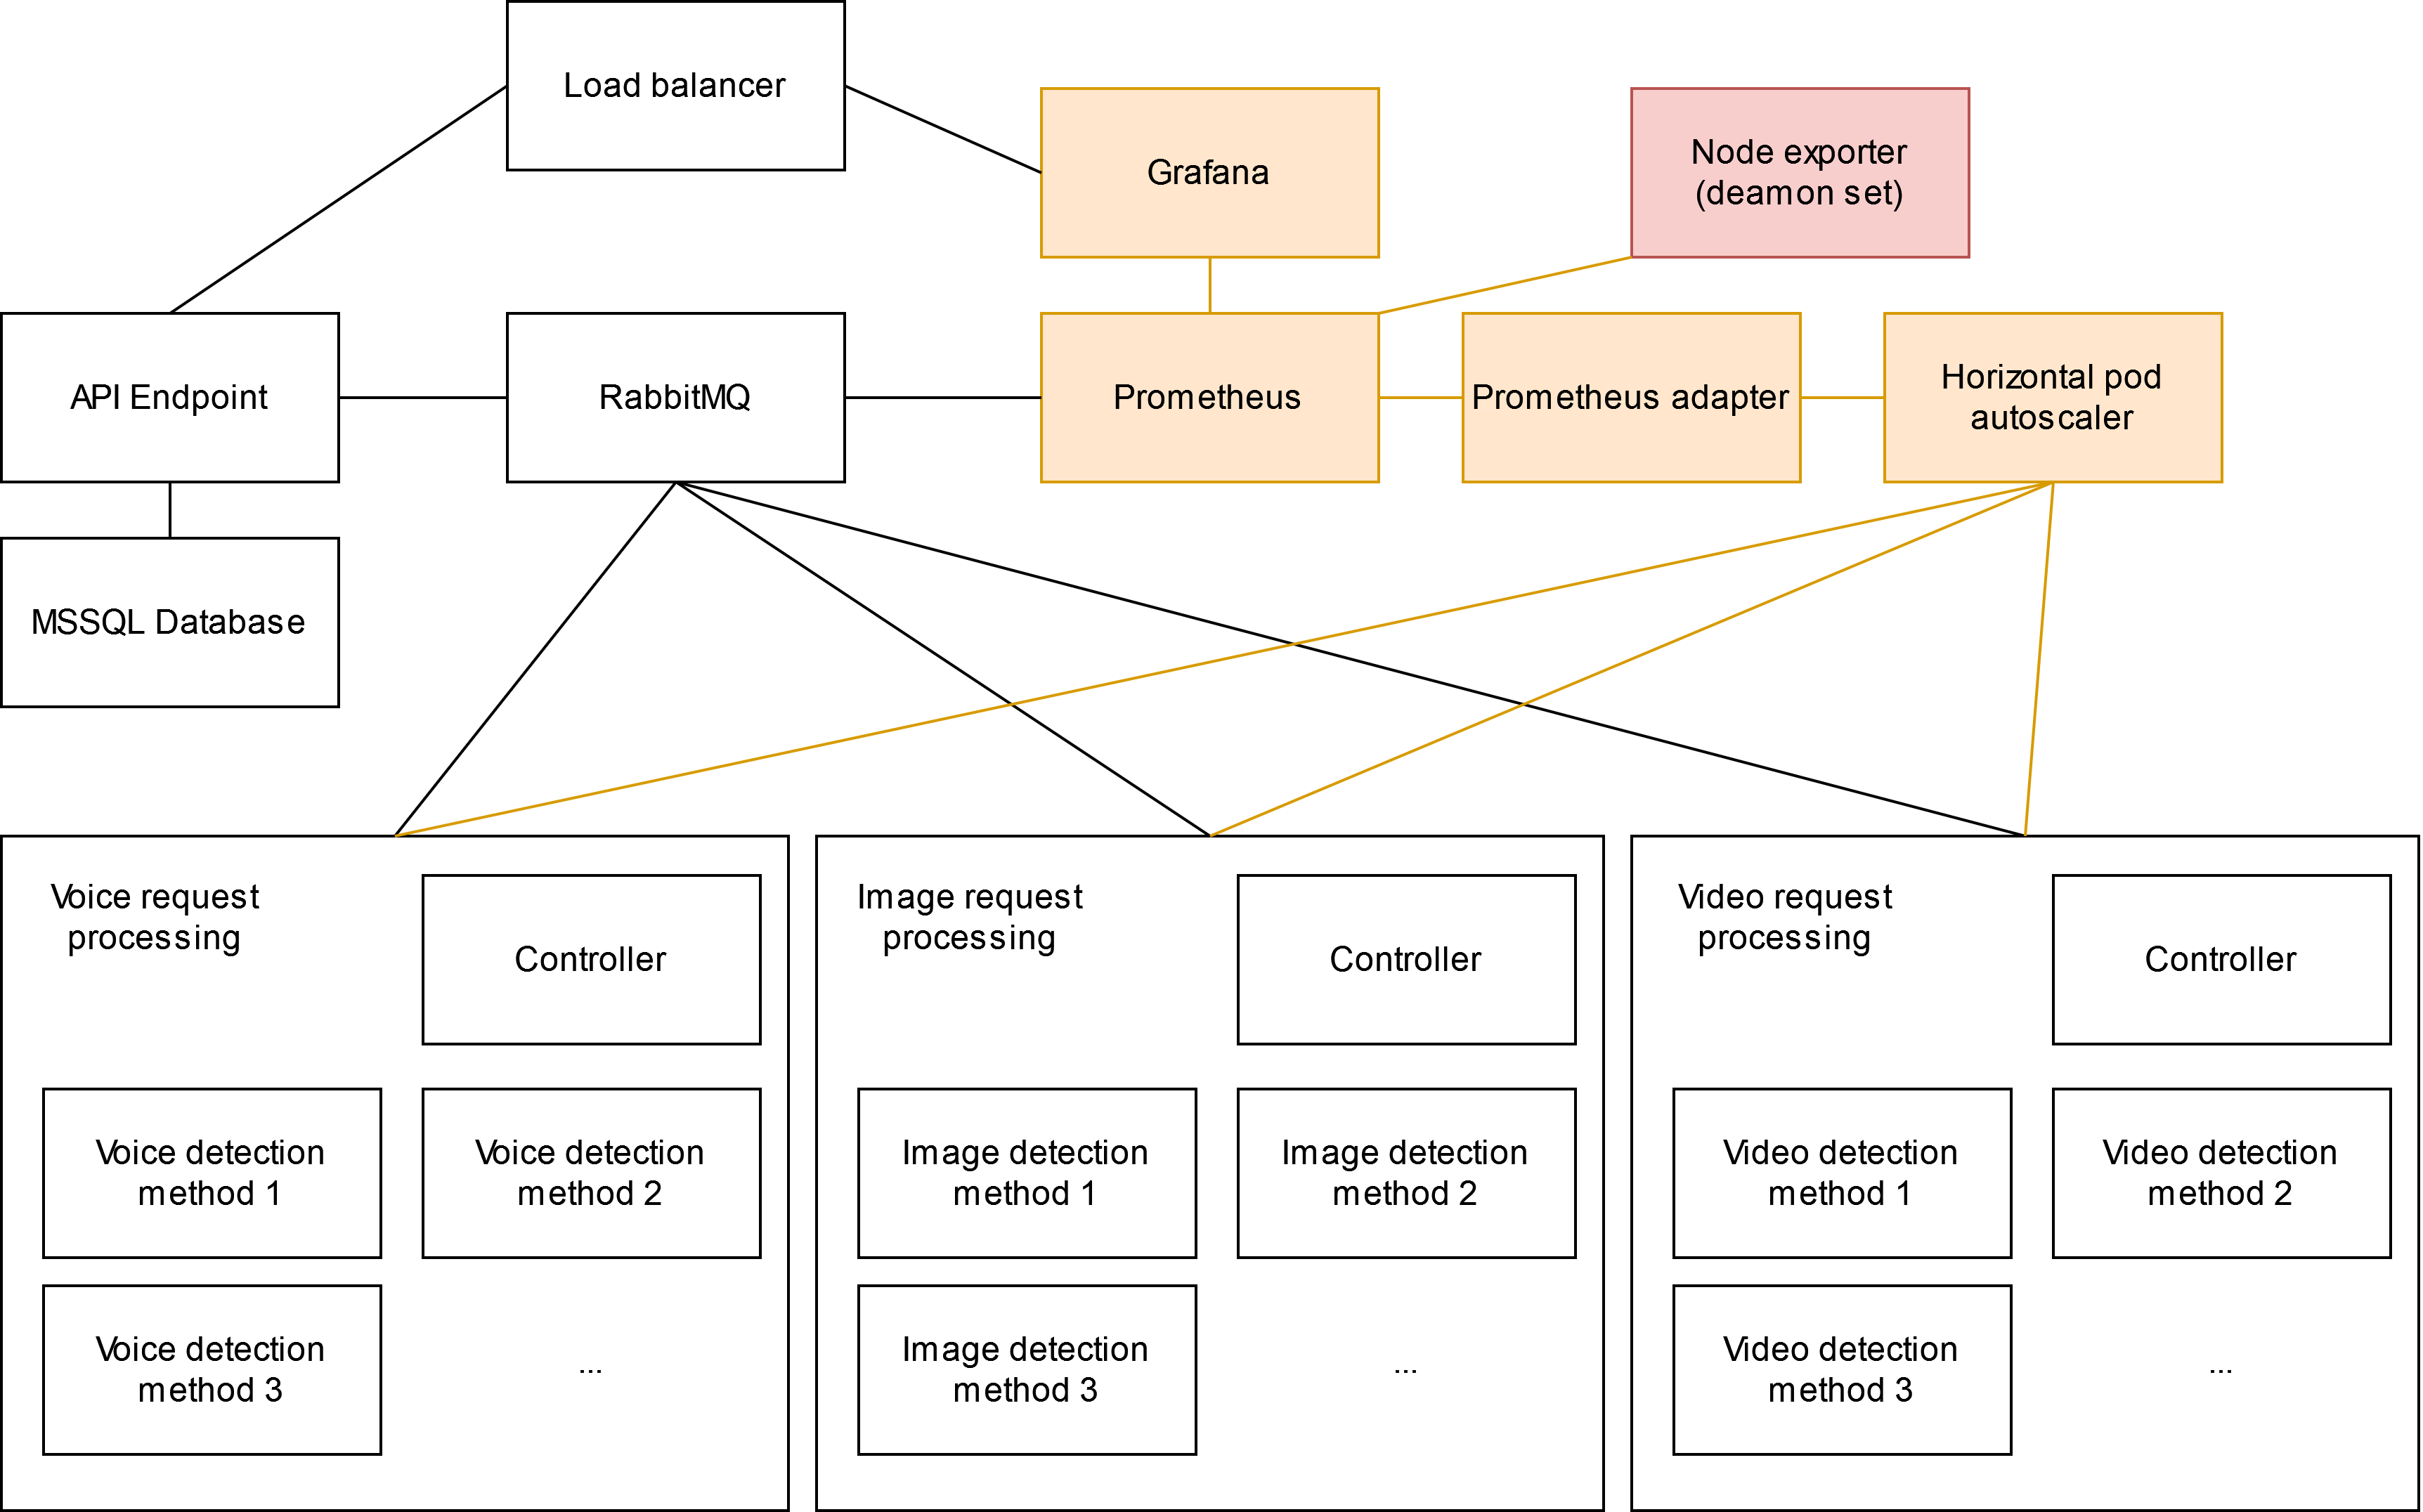
\includegraphics[width=\linewidth]{other-fig/framework_implementation.png}
    \caption{Diagram of implemented framework}
    \label{fig:framework_implementation}
\end{figure}

The framework was implemented on the previously defined architecture. The architecture primarily dealt with the main functionality of the framework, but it also covered supporting systems, for example, systems for collecting metrics used in scaling, etc. The overall implemented platform can be seen in diagram in fig.~\ref{fig:framework_implementation}. The system could be divided into two parts: processing - API endpoint, message broker, processing units (white rectangels), and monitoring - metric collector, observability platform, etc. (orange/red rectangels).

The individual parts are described in more detail in the following sections. The whole system is designed to work in Kuberentes, the container orchestration tool. The overall implementation involved the development of an endpoint API and a processing unit controller. Subsequently, it was necessary to configure other systems, such as the message broker, the database, or the metrics collector. Finally, it was necessary to integrate the different selected detection methods; for this purpose a templates were created to make the integration as simple as possible.

In the following sections, you will see terms related to Kubernetes; you will get an more detailed overview of them in section~\ref{section:deployment}. These are terms such as Kuberentetes object, operator, or API.

\section{API endpoint}

The interface for the client applications is a REST API developed in ASP.NET Core 7 with EF Core for relational object mapping over the MSSQL database. The RabbitMQ.Client nuget package is used to communicate with the RabbitMQ message broker. The application uses a software architecture similar to MVC, but without a view implementation. Views are completely replaced by the client application, but it is handled separately. API is split into two Visual Studio projects: first contains bussinies logic (controllers, services, etc.) and second one defines all data models. Controllers receive HTTP requests containing individual input parameters that are mapped to objects called viewmodels. When mapping to a viewmodel or directly after it, validations are performed. These include type checking, input length, or when uploading a file, checking for pairs of supported extensions and MIME Types.

If all input data is correct, the query processing can continue. In case of detection, the file is saved to a shared storage where the API endpoint is the only one with write permissions. Other parts of the framework can only read from this storage. The SHA256 checksum of that file is then calculated and compared against the database records. If this checksum is already in the database, the request ID containing this checksum is returned and the file is deleted. When the client queries the results, it gets the answer immediately because it is already in the database and the system is not unnecessarily overloaded with recomputation. However, if the checksum is not found in the database, a new request is created with the status \texttt{processing} and stored in the database. Subsequently, a message is sent via the message broker forcing the detection of this file. The message contains the same information as the database request (id, checksum, filename, status, type).

The OutputService class implements a function that handles the background consumption of messages containing results. When the server starts, it registers an event handler that is called when a message is received in the outuput queue. All the results are stored in the database and the status of the processed request is also changed to \texttt{done}. It is also necessary to delete the detected file from the shared storage. The incoming message contains the request ID and a list of responses, where each individual response contains the ID of the detection method and the resulting value. The list may also be empty, indicating an error or that a single method was unable to process the file. Detection methods can only support processing certain file types, so if no method is able to process the file, the list will be empty.

The results are issued to the client upon request via the \texttt{/requests/results} endpoint. In case the request processing is not complete, an empty response (HTTP 204) is returned. After (un)successful processing, an object containing the request ID, the overal score, and a list of results consisting of the detection method ID, the detection method name, the description, the name of the training dataset, and the result value is returned to the client. Information about the detection method is read from the configuration file \texttt{appsettings.json} based on detection method ID. The client must perform long pooling until it receives the first non-empty response. The client should timeout in case of a complete system failure.

Configuration file \texttt{appsettings.json} contains connection strings to database and RabbitMQ, definition of supported file types and detection methods details.

\section{Message broker}

RabbitMQ was selected as the message broker, which is designed for asynchronous messaging. Individual messages are stored in a message queue where producers insert them. The messages are then read by the consumers. The AMQP protocol is used for communication, which defines the structure of messages, their acknowledgement, etc~\cite{AMQP}.

RabbitMQ is designed to send a large number of small messages. It would not be appropriate to send, for example, a whole file in BASE64 encoding through it. Therefore, the file to be detected is stored on shared storage and a message containing the remaining necessary parameters is sent through the message broker. Then, consumers are scaled based on the number of messages in each queue to handle requests as quickly as possible.

Four different message queues are used for communication: \texttt{queue\_audio}, \texttt{queue\_image}, \texttt{queue\_video}, and \texttt{queue\_output}. On the basis of the file type, the API endpoint decides which queue the request should be placed in. The individual queues are then consumed by the individual controllers in the request processing units. The results are sent back to the API endpoint through the output queue.

The RabbbitMQ Cluster Operator provides a simple deployment to Kuberentes by defining new Kuberentes objects. The complete deployment manifest for RabbitMQ includes configuring the number of container replicas, default credentials, and setting resource usage limits. More details about deployment is in section~\ref{section:deployment}.~\cite{RabbitMQOperator}

\section{Processing unit}

The controller is implemented as a single file Python script. The same functionality could be implemented in C\# as well, but for this use case, using a scripting language was more straightforward. It is a script that receives a request and distributes it among the different detection methods. The pika library is used to communicate with the message broker.

It first establishes a connection and then connects to a given channel for which the QOS is set to 1. This indicates that it is able to consume only one message at a time. When calling the \texttt{start\_consuming} function on opened channel, the script starts listening on that channel for new messages. When a message is being consumed, a new thread is created that does not prevent the library from functioning. Pika needs to be be able to send regular heartbeat messages.~\cite{Pika}

The new thread will only start processing the request itself. Since the message sent is in JSON format, the request is mapped to a dictionary. Using the asyncio and aiohttp library, the HTTP endpoints of each detection method are called asynchronously. Since everything is stored in a single pod, the localhost interface is used for this communication. The ports of each detection value are read by the controller from an environmental variable that is defined in the Kubernetes manifest. The HTTP request contains all the defined parameters, and as a result an object containing the detection method id, request id and value decimal number is expected. When detection is complete, the individual results are stored in a list, which is converted again to JSON and sent to the output queue when all methods are done.

\section{Monitoring}
In order to scale, it is necessary to have metrics on which to scale. Every cloud service provides some form of monitoring and metrics collection, but since we don't want to be dependent on the platform on which the framework will be hosted, we need to configure the application to collect metrics on its own. For this case, the Prometheus platform was chosen.

Prometheus collects the defined metrics and stores them in a time series database. It can store metrics for several years. In our case, our interest was to collect RabbitMQ metrics that can be used for scaling and resource consumption of each cluster node. On the basis of the resource consumption, we are able to better allocate resources to different parts of the framework. 

Prometheus provides what is called the Prometheus Operator, which, as with RabbitMQ, simplifies the deployment of this application. After deploying the operator to a Kuberentes cluster, it is possible to create objects of type Prometheus. For a description of the deployment, see~\ref{section:deployment}.~\cite{PrometheusOperator}

The RabbitMQ Cluster Operator automatically collects metrics, and we only need to configure API for providing compatible metrics to Prometheus. Then only all you have to do is to create new Kuberentes service monitor object which actually enables these metrics consumption by Prometheus. The metrics contain data about the number of connections, the number of open channels, the number of messages in each queue, and much more. Number of unconsumed messages in queue was chosen for scaling. This value needs to be exposed to the Kubernetes API, which is not done by default.

To do this, it was necessary to incorporate a Prometheus Adapter that reads the selected metrics and makes them available to the Kubernetes API. More about it is in section~\ref{section:scalability} 

Node Exporter allows collecting metrics of resource usage of individual cluster nodes. If we configure Node Exporter container as a deamon set in a cluster, this container is then deployed to all running nodes in the cluster. The container must be configured with access to \texttt{/proc} and \texttt{/sys} virtual Linux directories from which it can retrieve individual metrics. Another service monitor object add these metrics to Prometheus the same way as for RabbitMQ.~\cite{NodeExporterSetup}

Prometheus is a good tool for collecting metrics, but its representation is not very good. In its web interface, it allows query calls that can be represented, for example, as a graph or just the current value. Grafana was chosen to represent the data from Prometheus. 

Grafana is the only one that requires manual configuration. First, it is necessary to access the web interface and enter the default login credentials. After that, a request to change password will pop up. After the change is made, a new data source must be configured in settings. Select prometheus and enter its domain name in the kuberentes cluster, which is “\texttt{http://prometheus-service.default.svc.cluster.local}”.

The user community shared the dashboards created on the official Grafana website, where it was possible to find the official dashboard for RabbitMQ and also the community dashboard for Node Exporter. Both dashboards provide a representation of a large number of metrics using charts, etc., which were sufficient for our needs. Fig.~\ref{fig:grafana_node_exporter} shows Grafana web interface with Node Exporter dashboard. It would be possible to create a custom dashboard containing selected metrics if needed.

\begin{figure}[H]
    \centering
    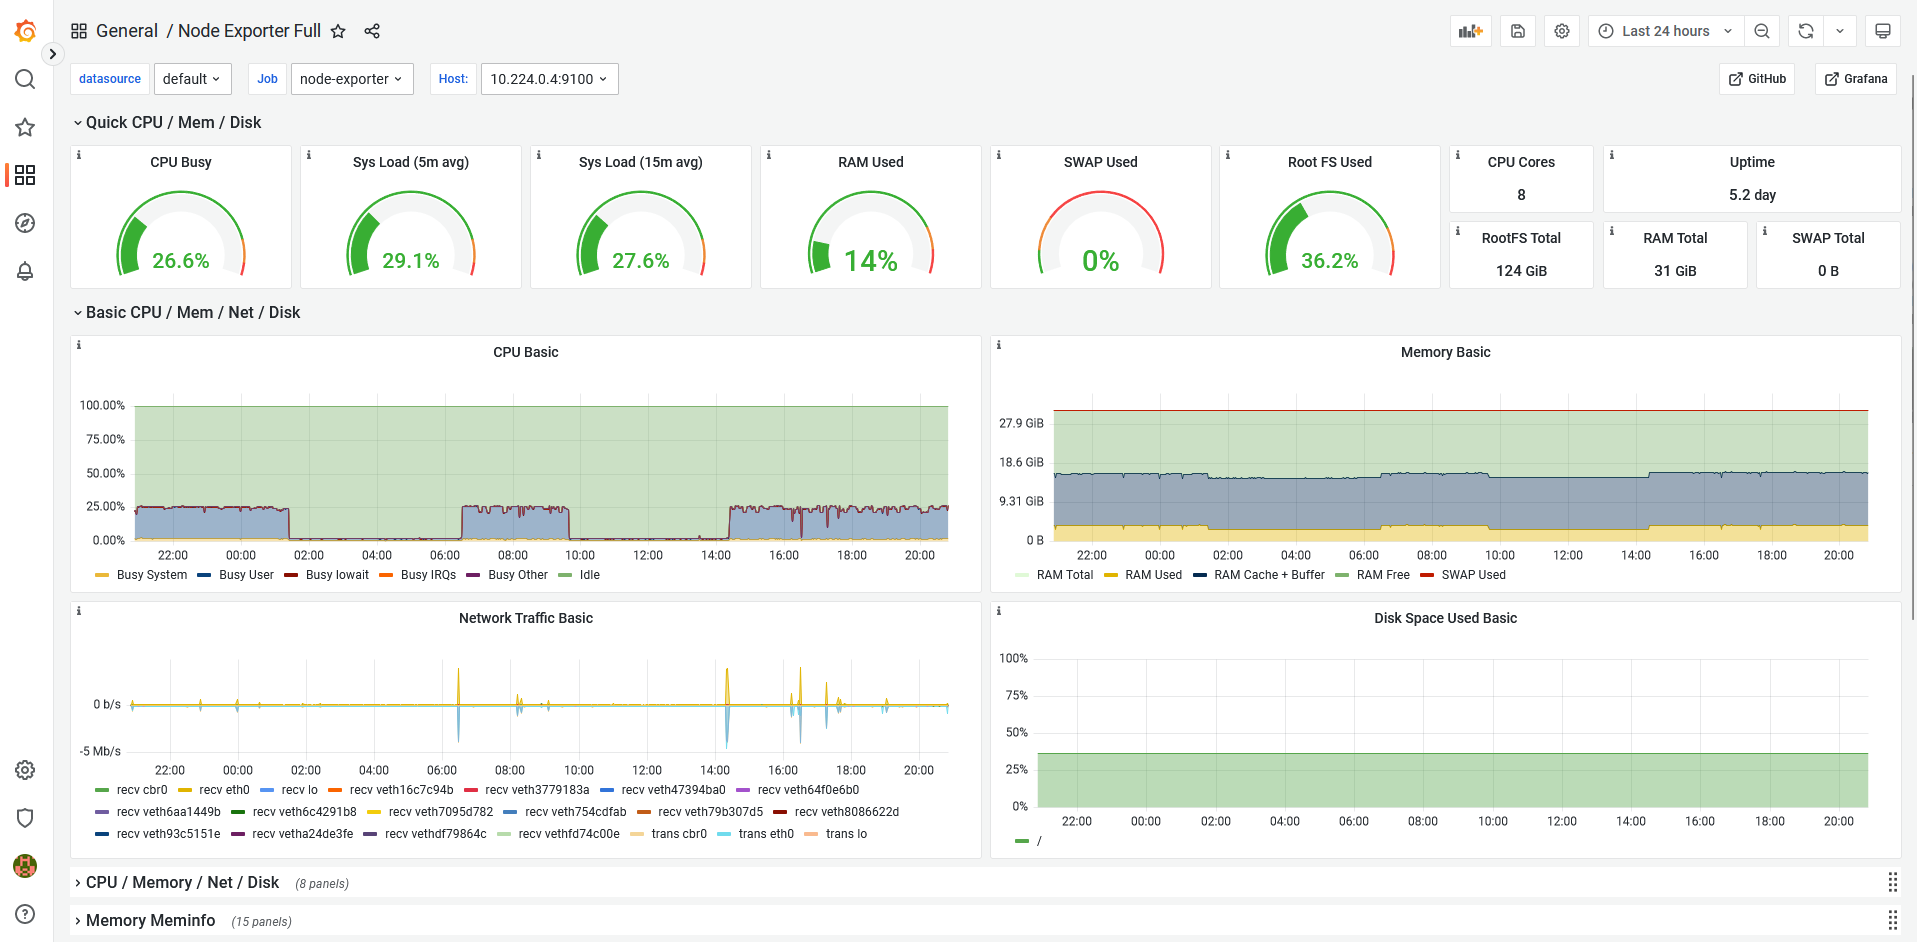
\includegraphics[width=\linewidth]{other-fig/grafana.png}
    \caption{Grafana - Noede Exporter dashboard}
    \label{fig:grafana_node_exporter}
\end{figure}


\section{Scalability}
\label{section:scalability}

The Prometheus Adapter is designed as a priority for deployment using the helm chart tool, which extends the capabilities of the kubernetes manifest files. To keep the deployment as simple as possible and to avoid having to use many different tools, all deployment files have been copied from the Prometheus Adapter repository to the framework repository. With some modifications, it was possible to get Prometheus adapter working using only Kuberentes manifest files.

Config map object for deploying Prometheus Adapter contains configuration such as name, which metrics and how they should be published, etc. Publication to Kubernates API was achieved by creating a Kubernetes object of type APIService. Testing whole integration is possible by using the command~\cite{PrometheusAdapter}: 

\begin{lstlisting}
kubectl get --raw /apis/custom.metrics.k8s.io/v1beta2 
\end{lstlisting}

\noindent Example results is shown in list.~\ref{list:kubectl_metrics}.

Horiznotal Pod Autoscaler needs several attributes to work. First, it is the identification of the object to be scaled and on what metric~\cite{HorizontalPodAutoscaler}. We have defined the name of the metrics in the Prometheus Adapter configuration map. Then we need to specify the minimum and maximum number of replicas and the average value. These values are then used in number of replicas calculation. In our case, minimum number of replicas is set to 1 and the maximum to 3. Average value of the messages in the queue is set to 2. These values can be modified according to the needs and environment in which the framework will operate.~\cite{HorizontalPodAutoscaler}

\begin{lstlisting}[caption={Result of calling the command to get metrics},label={list:kubectl_metrics}]
{
    "kind": "APIResourceList",
    "apiVersion": "v1",
    "groupVersion": "custom.metrics.k8s.io/v1beta2",
    "resources": [
        {
            "name": "jobs.batch/rabbitmq_metrics_audio_queue_depth",
            "singularName": "",
            "namespaced": true,
            "kind": "MetricValueList",
            "verbs": [
                "get"
            ]
        },
        ...
    ]
}
\end{lstlisting}


\section{Deployment}
\label{section:deployment}

The deployment of the entire framework is divided into several Kubernetes manifest files, where individual Kubernetes objects are defined. These are persistent entities that represent parts of the system, and each object is of a specific type. The basic types are, for example, pod, service, deployment, etc. If we want to work with these objects, we can only do so through the Kubernetes API. It is possible to define a new API in Kuberentes and other new object types in it. This functionality is used by so-called operators, which are designed to automate repetitive procedures or to facilitate the deployment of a more complex system into another. When deploying this solution, it is important to consider that the RabbitMQ Cluster Operator and Prometheus Operator were used. Both operators have prepared manifest file which enables deployed via one command.~\cite{KuberentesObject}

Two bash scripts were created to make deployment and deletion easier. In deployment both operators are applied to the cluster and then the whole framework is deployed from all manifest files. Pulling all images, allocating resources and spinning up containers takes a while. It can take several minutes to start everything up and because some containers are started earlier then other ones, it can cause their failuer. Failed containers will be automaticly restarted and the whole system then should be fully operational. 

To communicate with the Kuberentes API, you can use the \texttt{kubectl} tool, which provides options for creating or deleting objects, reporting cluster status, or more detailed descriptions of individual objects. Some parts of the framework require persistent storage, such as shared storage for discovery files or databases. For this purpose, Kuberentes provides objects of type PersistanceVolume and PersistanceVolumeClaim. Kubernetes allows the creation of so-called Storage Classes when installing a cluster, which automatically create a PersistanceVolume when a request is made to create a PersistanceVolumeClaim. Different cloud providers provide different Storage Classes depending on the usage needs (speed, availability, backup, etc.), and it is possible to modify the configuration of these objects during deployment. Manual creation of PersistanceVolume without Storage Class is also possible, but requires more complex setup of the cluster itself or custom storage outside the cluster. We will not develop this option further.

The deployment of the framework, if we omit the Prometheus Adapter, is divided into ten different manifest files.  Among the most important objects created are the deployment type objects that create individual pods, allow you to set the number of replicas (automatically using scailing or manually) and can be connected to the Kuberentes load balancer, etc. Other essential objects types are Service, RabbitMQ, Prometheus, possibly ServiceMonitor, HorizontalPodAutoscaler and DeamonSet.

For deployment, it is recommended to use the prepared srcipt \texttt{deploy.sh}, but if you need to manually interfere with the already deployed framework, you can use the tool “\texttt{kubectl apply -f <path>}” to apply a specific manifest file or folder. On the other hand,  “\texttt{kubectl delete -f <path>}” is used for removal.

The Endpoint API and Processing Request Controller are built into a Docker image using Github Action, which is then published to the GHCR public container registry provided by Github. Any change pushed to the main branch of the repository will trigger this pipeline. These images are configured in Kuberentes manifests, which makes it easy to deploy the latest version of the framework. If only one component is being updated, such as the API Endpoint, just stop and start the component again with “\texttt{kubectl delete}” and “\texttt{kubectl apply}”, which will cause the latest version of the container to be downloaded from the registry.

% ----------------------------------------------------------------------- %
\chapter{Detection methods integration}

Integrating the detection method only requires a container with an exposed REST API endpoint with one GET method (\texttt{detect}) on a specific port. This container image then needs to be correctly configured in the deployment files. Since this is a multicontainer pod, it is necessary that each detection method has its own port. There is a sample Dockerfile and one Python script with FastAPI library in the \texttt{template} folder. This script contains only one GET method with the given parameters mapped from the URL query parameters (id, checksum, filename, status, and type). Most of the parameters will probably not be used; the important ones are ID (request ID) and filename, which is the filename for deepfake detection saved in shared storage.

Template contains designed pipeline such as data preparation, detection and results normalization/generalization. If the method evaluates at any step of pipeline that it is unable to continue processing, either because of the file type or an internal error, it should correctly terminate the work and return \texttt{null} as the result. If processing is correct, it will return a detected value between 0 and 1. Result object should also return the ID of the detection method, which allows the Endpoint API to associate this result with a description of the detection method. This template does not need to be used and can be replaced by another technology more suitable for certain cases. It is a functional demonstration of how the integrated method should work.

\begin{lstlisting}[caption={Container configuration in Kubernates manifest},label={list:detection_method_manifest}]
- name: dfdf-detection-audio-2
  image: path/to/container/registry:main
  imagePullPolicy: IfNotPresent
  resources:
    requests:
      memory: "3.25G"
      cpu: "500m"
    limits:
      memory: "3.25G"
      cpu: "500m"
  volumeMounts:
    - name: processingdata
      mountPath: /mnt/processingdata
      readOnly: true
\end{lstlisting}

Subsequently, the container must be built and published to a registry accessible from the Kuberentes cluster. Depending on the type of detection method, it must be configured in a given deployment file. The project has three different deployment files according to file type: \texttt{processing-unit-voice.yaml}, \texttt{processing-unit-image.yaml}, and \texttt{processing-unit-video.yaml}. It should be mentioned that the size of the resulting container should not be too large. Otherwise, it causes problems with the speed of the deployment itself. If deployment of request processing unit is slow, then scaling will not be so effective. The Docker image must be downloaded from the registry, and this takes some time; the smaller the image, the less this operation will affect the speed of creating a new pod.

Adding a new container to the list in the “\texttt{spec.template.spec.containers}” section ensures that it will be part of the pod. You need to define the Docker image, the amount of resources the container can consume, and you also need to mount a shared repository where the files will be ready to be detected. Storage should be mounted in read-only mode. In list.~\ref{list:detection_method_manifest} you can see an example of configuration of one detection method. The controller needs to know that a new method exists so that the port where API is exposed has to the be added to environmental variable for the controller container. The variable is called „ProcessingUnitsPorts“.

\begin{lstlisting}[caption={Detection method description in appsettings.json},label={list:detection_method_description}]
{
    "ID": 1,
    "Type": 1,
    "Name": "Detection Method XX",
    "Description": "This is awsome detection method...",
    "TrainingDataset": "Training dataset XYZ"
}
\end{lstlisting}

In the last step of the integration, you need to update the \texttt{appsettings.json} file in the Endpoint API by adding the detection method description. The description includes the ID, which must be unique, type, name, description, and the name of the training data set. The type can take values: 0 = audio, 1 = image, 2 = video. An example can be seen in list.~\ref{list:detection_method_description}.
\section{AudioDeepFakeDetection}

This project\footnote{\url{https://github.com/PlayerBerny12/AudioDeepFakeDetection}} implements different types of models and combines them with different feature extractors. The project provides six different neural network models and three different feature extraction methods, providing a considerable number of combinations to create different detection methods. This project was chosen because it offered great potential for trying different detection methods and the code was relatively easy to understand at first glance. The project describes well the steps needed to make it work, which led to success without any problems after replication.

The problem with most open source detection methods is that they are scientific papers and not tools for ordinary users. For optimization, these tools work with batches of files at a time, both in learning and in verifying the results. This leads to the fact that these methods cannot verify only one file as a rule. This is not different in the case of AudioDeepFakeDetection. Therefore, it was necessary to start modifying the code. A fork of the repository was created in which this change was made. A function was created to allow only one file to be processed.

The project provided pre-trained models for download, but these were not used. The datasets used for training were LJ Speech and WaveFake. A more detailed description of the datasets can be found in section~\ref{section:datasets}. When replicating the experiment, 6 different detection methods were eventually created. Combinations of the most successful models and feature extractors based on output of their experiments were selected. Each method was trained for 15 epochs. All methods had the highest achieved accuracy of over 90 \% on the test dataset, some even very close to 100 \%. The training results are presented in tab.~\ref{table:training_results}. The first part of the name indicates the name of used model, the second part is name of the feature extraction, and the last part can take two values: I = in distribution, O = out distribution.

\begin{table}[H]
    \centering
    \begin{tabular}{|l|r|r|r|r|}
        \hline
        Experiment & \multicolumn{1}{l|}{Accuracy} & \multicolumn{1}{l|}{F1} & \multicolumn{1}{l|}{ROC AUC} & \multicolumn{1}{l|}{EER} \\ \hline
        ShallowCNN\_mfcc\_O & 0.942 & 0.941 & 0.9418 & 0.0743 \\ \hline
        ShallowCNN\_lfcc\_O & 0.949 & 0.949 & 0.9494 & 0.0647 \\ \hline
        TSSD\_wave\_O & 0.958 & 0.958 & 0.9576 & 0.0462 \\ \hline
        TSSD\_wave\_I & 0.997 & 0.997 & 0.9969 & 0.0042 \\ \hline
        ShallowCNN\_mfcc\_I & 0.997 & 0.997 & 0.9971 & 0.0053 \\ \hline
        ShallowCNN\_lfcc\_I & 0.999 & 0.999 & 0.9994 & 0.0008 \\ \hline
    \end{tabular}
    \caption{AudioDeepFakeDetection training results}
    \label{table:training_results}
\end{table}

The training and test dataset are created automatically from the two provided datasets. The split was in the simplest possible way, the first part of the data was labelled as training, and the second as testing. The parameter \text{in\_distribution} also influenced whether the distribution of deepfake and originals was 1:1 or 7:1 in favor of deepfakes. Training 15 epochs on the Nvidia GeForce GTX 1660Ti graphics card took around 9 hours. For example, the model \texttt{ShallowCNN\_lfcc\_I} was trained from 8:04 AM to 4:58 PM (final time 8:54). All training logs can be found in the repository in the \texttt{saved} folder.

For the integration, 6 different Docker images had to be created. Prepared templates were used for this operation. An automatic build of the images in Github Actions when pushing any change to \texttt{master} branch was implemented. The images are then published in the GHCR container registry and can be embedded in the framework.

This project is built on the PyTorch library and the official PyTorch Docker image was used as the base for the image creation. After building this image, everything worked correctly and all methods processed the files in the framework in parallel. However, a problem arose, downloading the images to a given node. It turned out that the base PyTorch image was several gigabytes in size and with the model embedded, downloading the necessary \texttt{pip} package had a resulting size of 10.59 GB. Although some layers are shared between images, it took several minutes to initialize all 6 detection methods.

It was necessary to proceed to optimization. The PyTorch Docker image as the base image was replaced with a Python image. This was because it turned out that PyTorch contained all the necessary libraries to run on the graphics card, which were not needed. PyTorch was installed in the Python image to run only on the CPU and other minor optimizations were made, such as clearing the memory cache after installing the package, etc. Due to these changes, the size was reduced to 1.48 GB. This optimization reduced the deployment time to a maximum of tens of seconds in an environment with good connectivity from the cluster to the container registry.

\section{fakeVideoForensics}

The intgeration procedure for this project\footnote{\url{https://github.com/PlayerBerny12/fakeVideoForensics}} was the same as in the previous methods, perhaps a little simpler. Again, prepared templates were used, and an automated build was created using Github Actions with image publishing to GHCR container registry.

This method focusses on video detection, but provides no description of how the model should be trained. The repository probably does not even contain a script that could be used for this purpose. However, it was possible to use an already pre-trained model. This project focused on processing only one file, so no code changes were necessary, still fork of this repository was created.

The lesson learnt from previous integration of detection methods was to optimize the image size as a second step. The image created on the first attempt had 4.81 GB. We tried to use PyTorch without the ability to run on the graphics card, deleting the cache, etc. The success was not that great in this case, but we still managed to reduce the image size to 3.63 GB.

% ----------------------------------------------------------------------- %
\chapter{Client application implementation}

A browser add-on is actually a web application that has minor specifics. A must have is a "Web app manifest" that specifies what attributes and permissions the add-on has. The basic attributes are name, version, default popup file (this is the application's entrypoint file), etc. One of the permissions is the ability to access the DOM on the currently open or hosted page. This allows it to read and search for certain elements on the page or even modify them.

As the add-on does not require any specific permissions in the base, it is a normal web application. If interactive selection of elements on the page is implemented, then the application would require the use of special browser APIs.

The Angular Material framework with the Angular Material component library was used for implementation. This made it possible to create a simple, and most importantly, fast, visually appealing application. The application may not appeal to some, but its purpose was focused on simplicity and understandability. 

\section{Functionalities}

The app provides all the proposed functionality, but potential extensions were not covered. Thus, it is not possible to interactively select an element on the page to detect. Otherwise, it is possible to upload your own files or links. Once the detection is started the application displays a loading screen, once the request is processed, the results are displayed. The implemented application tried to keep the layout and functionality not designed in wireframes; it was not always technically possible. 

One difference from the design is the use of a dialog box instead of a tooltip. Angular Material does not allow for tooltip creation, and the use of another 3rd party library was deemed inappropriate for subsequent application maintenance. This is a minor change that is more technical in nature and does not affect the functionality in any way.

The second difference was in moving the button to send feedback from the bottom of the application to the top. During development, this location was identified as inappropriate because it obscured the results bars.

\section{Communication with framework}

The most specific part of the implementation of the application was communicating with the framework and waiting for the detection to complete. The application uses the so-called long pooling, it is a technique of repeatedly sending messages to the server to retrieve certain information. The application resends the message to the REST API using the "request/resutls" method and waits until it receives a non-empty response. Since processing is expected to take some time, the pause between calls was chosen to be one second. 

In the extreme case, a framework crash could occur, so a timeout should be implemented to maximize the wait time. The timeout value was set to 20 min. The timeout should not really occur, and it is a last resort to notify the user of a possible problem.

This communication could be replaced by websockets in the future, where resource wastage would be reduced in some way (by repeatedly sending HTTP requests) and the server could notify completion as soon as it receives processed results. Managing websockets is not free, but it would be possible to compare which technique is more efficient. 

\section{Supported browsers}

The add-on does not use a specific API to communicate with the browser, making the application more easily portable between different browsers. The functionality was tested in Google Chrome (v113), Microsoft Edge (v113) and Mozilla Firefox (v113). The add-on worked without errors in all browsers with one exception. It is not possible to upload a file in Mozilla Firefox because when the file picker is closed, the add-on itself is also automatically closed and the user is unable to view the results page in this case. This is bug\footnote{\url{https://bugzilla.mozilla.org/show_bug.cgi?id=1292701}}, which after a long time might be closed in one of the upcoming versions. Using the link to detect it works without any problems. 

Using the "npm run build" command, the project is built and in the "dist" folder, and it is possible to load the add-on in the browser when using the developer mod in browsers.

% ----------------------------------------------------------------------- %
\chapter{Test experiment and results}

Three different test scenarios were created to test the reliability of the framework, the resources consumed, the workload, and the accuracy of the detection methods. Five different datasets were used for the tests, which were then used to generate data for each test scenario. In total, more than 2200 files were run through the framework during the tests.

The following sections show the CPU load and RAM usage graphs from Grafana, unfortunately, the labels are hard to read in the document. The graphs should have a sufficient textual description to compensate for this deficiency. Alternatively, high-resolution images are available on the included media, where the labels should already be easy to read. In the case of the CPU load graph, the colors represent the following properties/values: yellow - busy system, blue - busy user, red - busy lowait, and green - idle. For RAM usage, on the other hand, the colors represent: yellow - RAM used, blue - RAM cache + buffer, green - RAM free. CPU load is in percentages from 0 to 100 \% and RAM usage from 0 to 32 GB.

\section{Datasets}
\label{section:datasets}

Five different datasets were used for testing; three audio datasets: LJ Speach, WaveFake, and ASV2021, and for video: FaceForensics++ and CelebDF. Some datasets were used when training each method; if this was not the case in the test scenarios, these data were not used where possible. For fakeVideoForensics, it was not possible to verify which dataset data was used for training, hence the accuracy of the method may be slightly higher if this data were used. To make the tests more provable, data from a dataset on which no learning was performed were always used.

For the first test scenario, 500 recordings/videos were selected from a given dataset, where 250 were deepfakes and 250 were originals. Thus, four sets of 500 files were created. For stress testing, 75 audio recordings and 25 from the WafeFake and CelebDF datasets were randomly selected. In this case, it was not the detection result that mattered, but the processing time.

The ASV2021 dataset contained FLAC recordings, but the detection methods included in the framework were unable to process this format, so they were converted to WAV format using the "ffmpeg" tool.

The LJ Speech and WaveFake datasets do not achieve high quality from today's perspective, because LJ Speech contains recordings of only one person. WaveFake is then a dataset generated based on LJ Speech applying different generation techniques. Perhaps this is why the detection methods in AudioDeepFakeDetection achieved such high values during training. Therefore, it will be interesting to see how these detection methods perform against ASV2021 recordings.

\section{Test case 1 - accuracy}

The first test scenario tests the reliability of the framework and the accuracy of each method. Four iterations of this scenario were performed, where each input data was from one dataset. One iteration took several hours to perform. Thus, one iteration contained the 500 files (250 originals, 250 defaults). The files were sent sequentially to the detection, thus always waiting for one file to finish processing before starting the next one. For each item, the processing time, the results of each detection method, and the file size were measured. ROC curves with AUC values were generated for each iteration and each detection method.

Four different total score calculations were also tested, with the best one selected and included in the framework. The first calculation used a weighted average, in which it prioritized the minimum value (deepfake) of all the resulting ones. The second calculation, on the other hand, prioritized the maximum value (original) using the weighted average. The third calculation took the average value of all methods. The last calculation combined all the previous three variants, and the calculation depended on how many methods were at the playing 50 % and how many methods were below it.

The first iteration was performed with data from the LJ Speech (250 originals) and WafeFake (250 deepfakes) datasets. During training, the data was automatically split in a very primitive way in training and testing. In the case of the "in distribution" type, only one type of deepfake was trained. Thus, we pseudo-randomly selected data from the testing part of the dataset.


\begin{figure}[H]
    \begin{subfigure}[h]{0.5\linewidth}
        \centering
        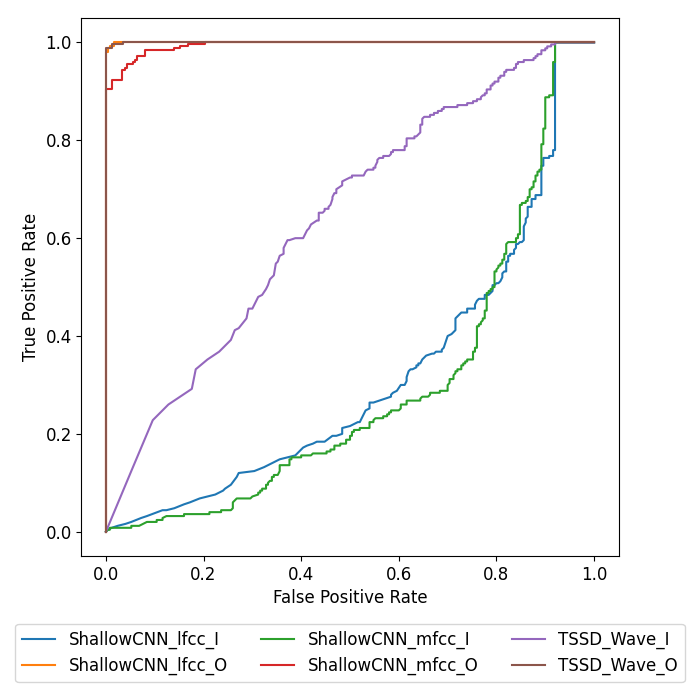
\includegraphics[width=1\linewidth]{other-fig/tests/lj_wf_methods.png}
        \caption{...}
    \end{subfigure}
    \hfill
    \begin{subfigure}[h]{0.5\linewidth}
        \centering
        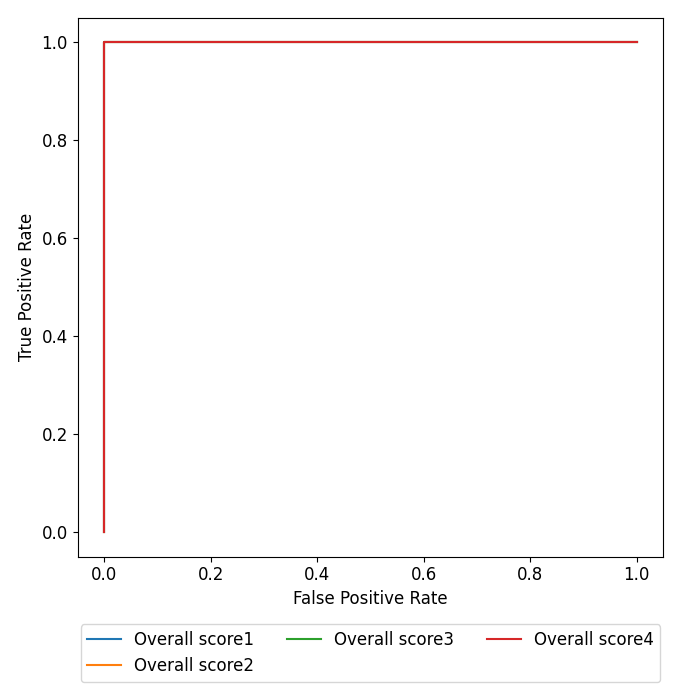
\includegraphics[width=1\linewidth]{other-fig/tests/lj_wf_overall_score.png}
        \caption{...}
    \end{subfigure}
    \caption{...}
    % \label{fig:subjective_answers}
\end{figure}
Some methods achieved very decent results; these are the methods that were "out of distirbution". The "in distribution" methods were trained on only one type of deepfake, which was minimally represented in the test data. The ShallowCNN model trained on only one type of deepfake was unable to generalize, and its results were very poor. All calculations of the overall score achieved a perfect classifier.

In table~\ref{} you can see statistics on the test data and the processing time.

\begin{table}[H]
    \begin{minipage}[c]{.5\textwidth}
        \centering
        \begin{tabular}{|l|r|}
            \hline
            Detection method & \multicolumn{1}{l|}{AUC} \\ \hline
            ShallowCNN\_lfcc\_I & 0.313040 \\ \hline
            ShallowCNN\_lfcc\_O & 0.999808 \\ \hline
            ShallowCNN\_mfcc\_I & 0.289784 \\ \hline
            ShallowCNN\_mfcc\_O & 0.994016 \\ \hline
            TSSD\_Wave\_I & 0.641496 \\ \hline
            TSSD\_Wave\_O & 0.999760 \\ \hline
            Overall score1 & 1.0 \\ \hline
            Overall score2 & 1.0 \\ \hline
            Overall score3 & 1.0 \\ \hline
            Overall score4 & 1.0 \\ \hline
        \end{tabular}
        \caption{xkj}
    \end{minipage}
    \begin{minipage}[c]{.5\textwidth}
        \centering
        \begin{tabular}{|l|r|}
            \hline
            Size average & 288.3 kB \\ \hline
            Size median & 299.5 kB \\ \hline
            Size minimum & 67.9 kB \\ \hline
            Size maximu & 445.0 kB \\ \hline
            Time average & 72.9 s \\ \hline
            Time median & 77.9 s \\ \hline
            Time minimum & 16.6 s \\ \hline
            Time maximum & 85.4 s \\ \hline
        \end{tabular}
        \caption{xkj}
    \end{minipage}
\end{table}

The total CPU load exceeded 60 \% almost all the time, of which about 20 \% was taken by system load and the remaining 40 \% by applications from user space. System load is likely to include resource management, throttling, context switching, etc. For RAM usage, we can see spikes reaching up to 30 GB if you include RAM Used and Ram Cache + Buffer. Memory is always freed up between detection runs, and we can see that PyTorch runs are relatively RAM intensive.

\begin{figure}[H]
    \centering
    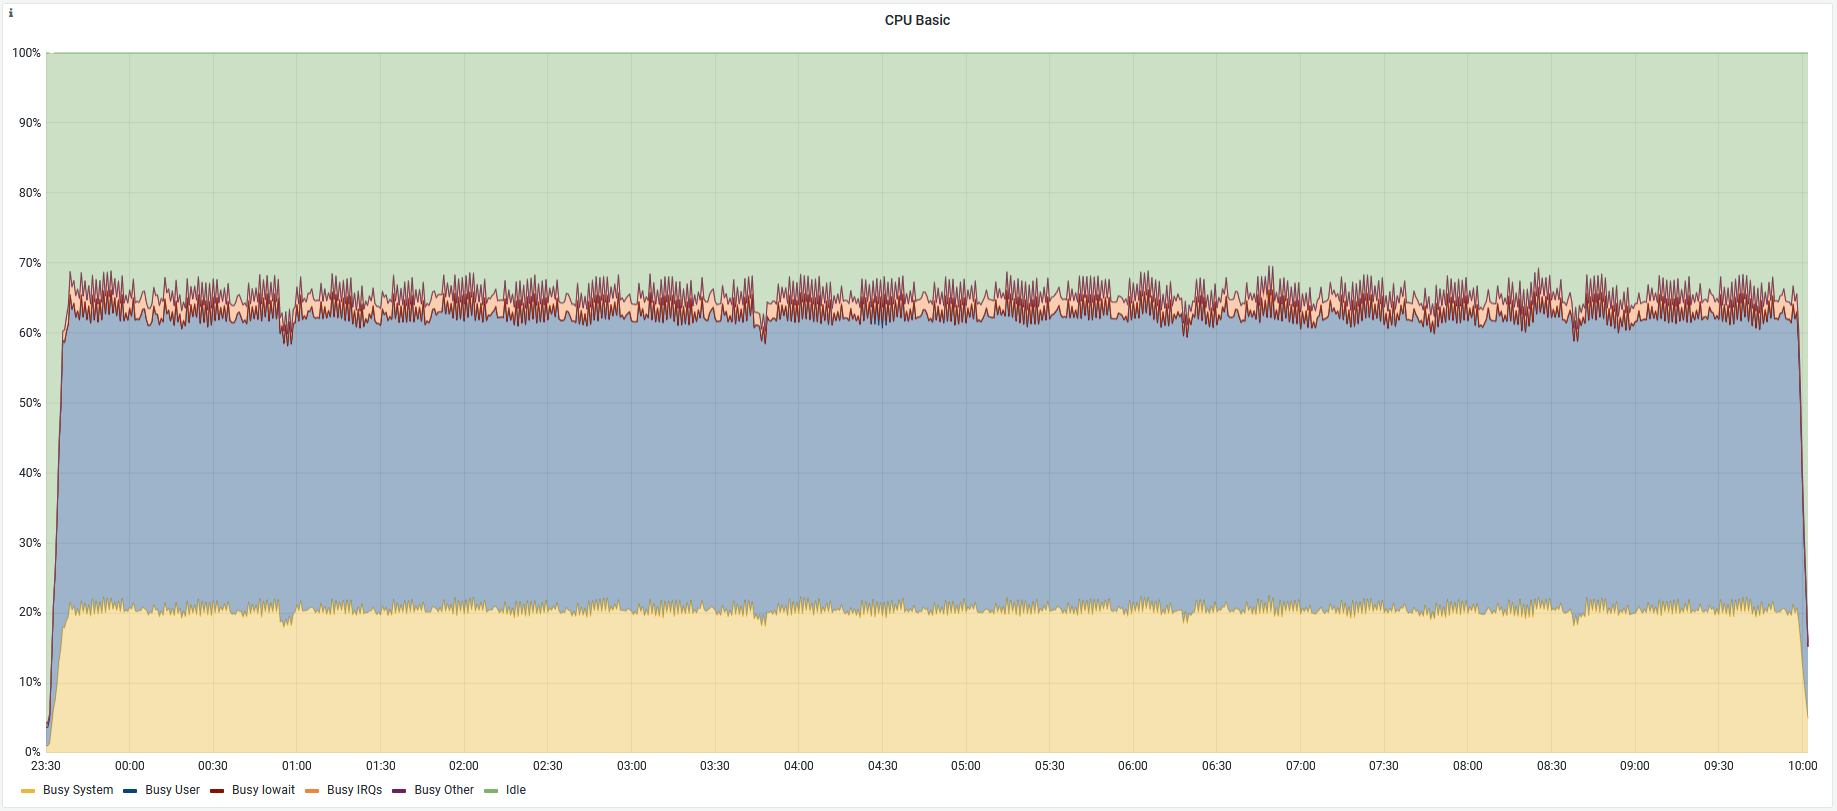
\includegraphics[width=1\linewidth]{other-fig/tests/lj_wf_cpu.png}
    \caption{...}
    % \label{fig:subjective_answers}
\end{figure}

\begin{figure}[H]
    \centering
    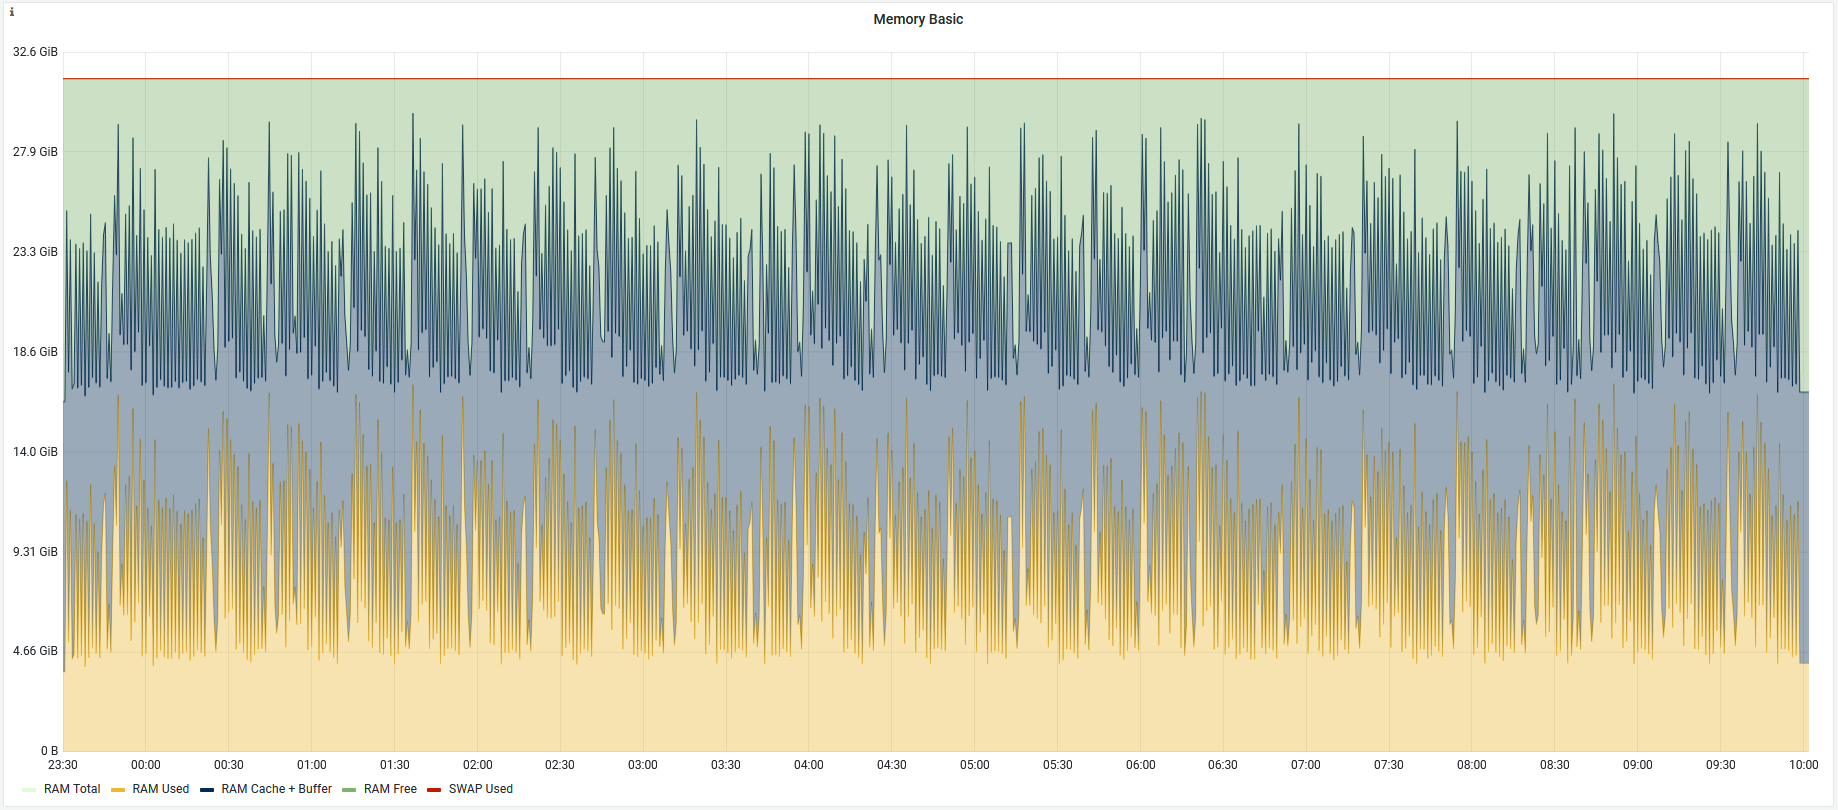
\includegraphics[width=1\linewidth]{other-fig/tests/lj_wf_ram.png}
    \caption{...}
    % \label{fig:subjective_answers}
\end{figure}

The second iteration used the ASV2021 dataset, which is divided into three parts. One part is the deepfakes, the second part is the original recordings, and the third part is the original recordings played back and resampled by the recording device. All three parts were used in the tests and where the originals and the re-recorded originals were in a 1:1 ratio.

The results are no longer as perfect as in the first iteration. It could be said that all the detection methods in this case are at the level of a random classifier. If we compare the two iterations, the \texttt{TSSD\_Wave\_O} detection method performs the best. This was a repeat of the experiment, but its real-world application is not particularly beneficial. Had these methods been trained on a more robust dataset, they might have had better results.

\begin{figure}[H]
    \begin{subfigure}[h]{0.5\linewidth}
        \centering
        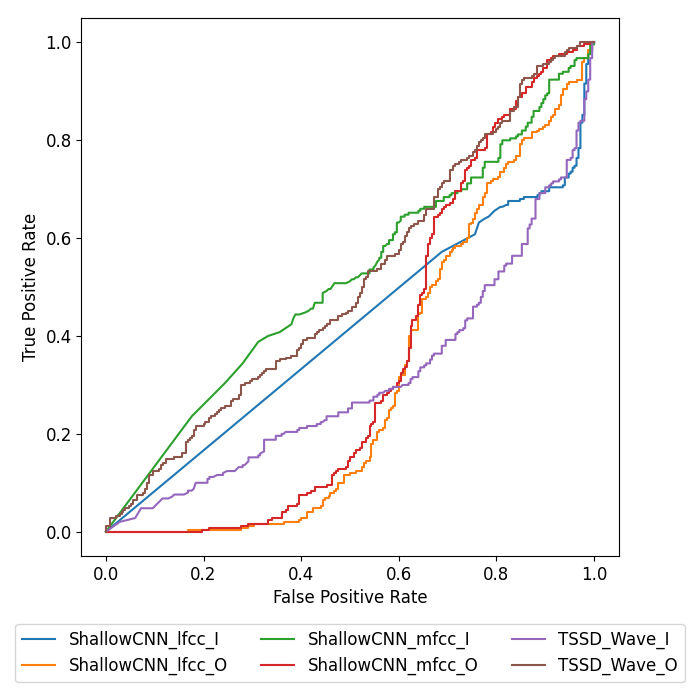
\includegraphics[width=1\linewidth]{other-fig/tests/asv_methods.png}
        \caption{...}
    \end{subfigure}
    \hfill
    \begin{subfigure}[h]{0.5\linewidth}
        \centering
        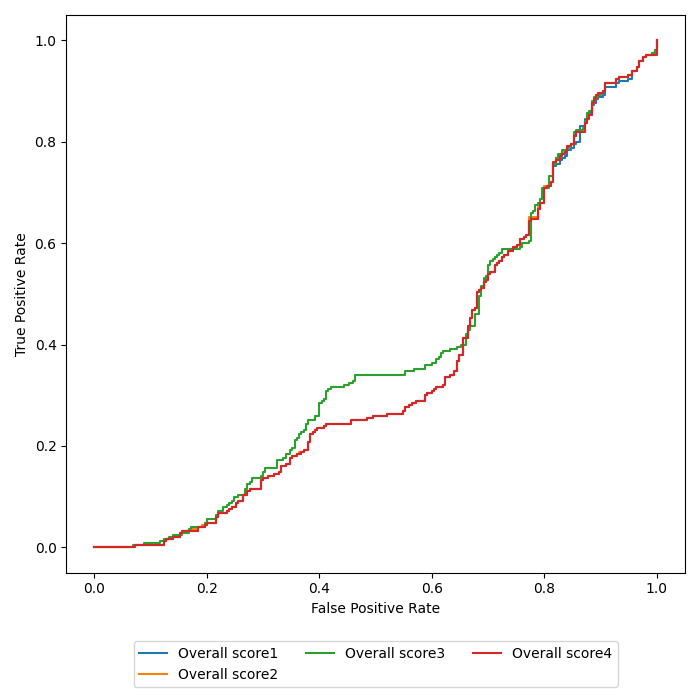
\includegraphics[width=1\linewidth]{other-fig/tests/asv_overall_score.png}
        \caption{...}
    \end{subfigure}
    \caption{...}
    % \label{fig:subjective_answers}
\end{figure}

\begin{table}[H]
    \begin{minipage}[c]{.5\textwidth}
        \centering
        \begin{tabular}{|l|r|}
            \hline
            Detection method & \multicolumn{1}{l|}{AUC} \\ \hline
            ShallowCNN\_lfcc\_I & 0.410944 \\ \hline
            ShallowCNN\_lfcc\_O & 0.305408 \\ \hline
            ShallowCNN\_mfcc\_I & 0.517672 \\ \hline
            ShallowCNN\_mfcc\_O & 0.349888 \\ \hline
            TSSD\_Wave\_I & 0.309056 \\ \hline
            TSSD\_Wave\_O & 0.507360 \\ \hline
            Overall score1 & 0.353648 \\ \hline
            Overall score2 & 0.354896 \\ \hline
            Overall score3 & 0.376416 \\ \hline
            Overall score4 & 0.354496 \\ \hline
        \end{tabular}
        \caption{xkj}
    \end{minipage}
    \begin{minipage}[c]{.5\textwidth}
        \centering
        \begin{tabular}{|l|r|}
            \hline
            Size average & 87.5 kB \\ \hline
            Size median & 78.5 kB \\ \hline
            Size minimum & 19.1 kB \\ \hline
            Size maximu & 265 kB \\ \hline
            Time average & 49.5 s \\ \hline
            Time median & 76.1 s \\ \hline
            Time minimum & 16.3 s \\ \hline
            Time maximum & 96.1 s \\ \hline
        \end{tabular}
        \caption{xkj}
    \end{minipage}
\end{table}

Interestingly, the calculations of the overall score are not particularly different, and the best performance is for the overall score based on a simple average. Perhaps if individual detection methods had performed a little better, then comparison of the total score calculation would be more telling. In this case, we cannot objectively declare one method to be the best. We think the fourth method might have potential and will therefore be implemented in the framework. 

The video detection method is only one integrated method, so we have no comparison. We could try to compare the results with Deepware, but unfortunately we were not given access to their API. We did a small manual test, but its comparison would not have much informational value.

The third iteration was done with selected data from the CelebDF dataset, and the fourth iteration from FaceForensics++. This detection method was learnt over the FaceForenicscs++ dataset, but unfortunately nowhere is it described what data were used for training; all or part, if any. Therefore, the selection was again done pseudo-randomly.

\begin{figure}[H]
    \begin{subfigure}[h]{0.5\linewidth}
        \centering
        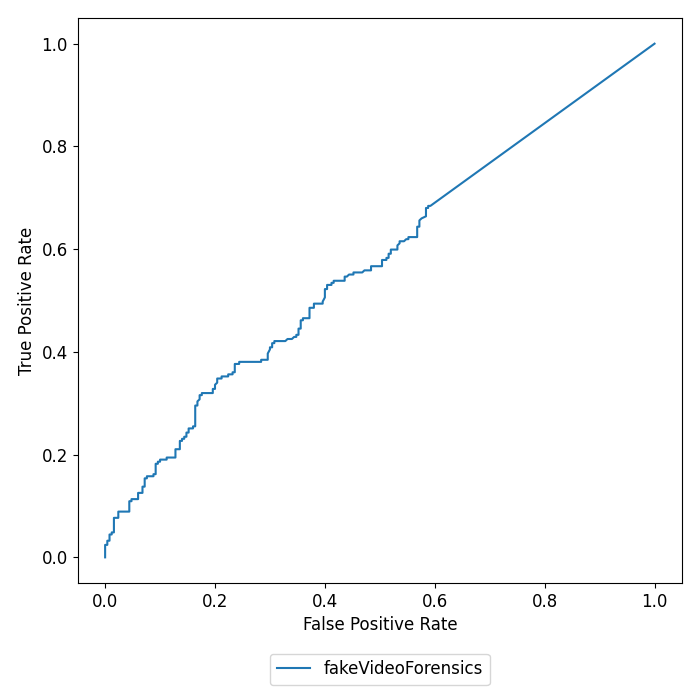
\includegraphics[width=1\linewidth]{other-fig/tests/cdf_methods.png}
        \caption{...}
    \end{subfigure}
    \hfill
    \begin{subfigure}[h]{0.5\linewidth}
        \centering
        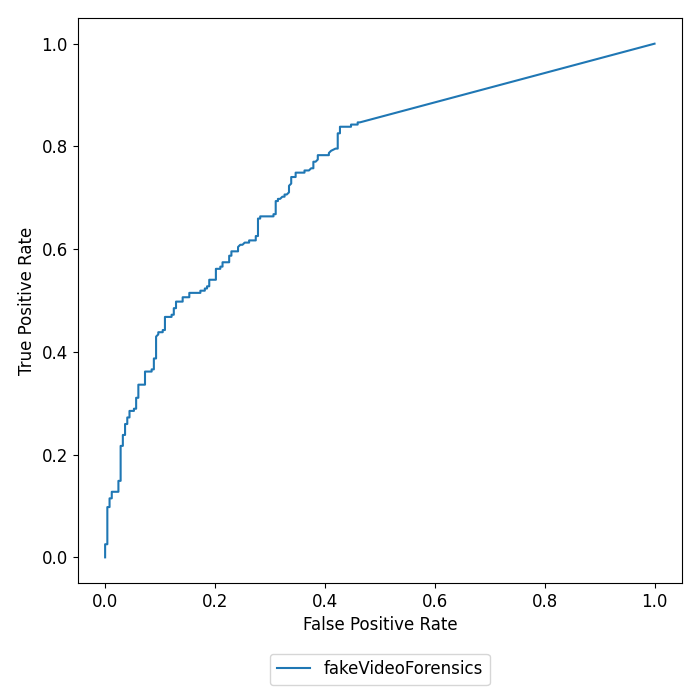
\includegraphics[width=1\linewidth]{other-fig/tests/ff_methods.png}
        \caption{...}
    \end{subfigure}
    \caption{...}
    % \label{fig:subjective_answers}
\end{figure}

The AUC values for the CelebDF data were 0.5738 and for the FaceForensics++ data 0.7584. As mentioned, the result for FaceForensics may be a bit biased because we do not know how much our test data overlap with the real training data. However, a result of around 60 \% could be considered acceptable.

\begin{table}[H]
    \begin{minipage}[c]{.5\textwidth}
        \centering
        \begin{tabular}{|l|r|}
            \hline
            Size average & 1893 kB \\ \hline
            Size median & 1674 kB \\ \hline
            Size minimum & 467 kB \\ \hline
            Size maximu & 5992 kB \\ \hline
            Time average & 153.8 s \\ \hline
            Time median & 145.7 s \\ \hline
            Time minimum & 34.6 s \\ \hline
            Time maximum & 496.8 s \\ \hline
        \end{tabular}
        \caption{xkj}
    \end{minipage}
    \begin{minipage}[c]{.5\textwidth}
        \centering
        \begin{tabular}{|l|r|}
            \hline
            Size average & 2031 kB \\ \hline
            Size median & 1559 kB \\ \hline
            Size minimum & 449 kB \\ \hline
            Size maximu & 10694 kB \\ \hline
            Time average & 389.5 s \\ \hline
            Time median & 305.3 s \\ \hline
            Time minimum & 126.4 s \\ \hline
            Time maximum & 881.7 s \\ \hline
        \end{tabular}
        \caption{xkj}
    \end{minipage}
\end{table}

Video processing took much longer and is at the limit of what is bearable for the average user. Averaging around three 3 minutes for the CelebDF data and 6.5 min for FaceForensics++. Yet the videos are by no means larger, very likely a more efficient codec or more compression is used, and the videos are that much longer.

On the CPU and RAM usage graphs, we can see that this method is slightly more efficient in RAM consumption, and hence we do not see the various spikes in the graph. Since there is no need to solve multiple detection methods in parallel in different containers, the CPU usage of the system is minimal and 20 \% is taken by the detection method itself.

\begin{figure}[H]
    \centering
    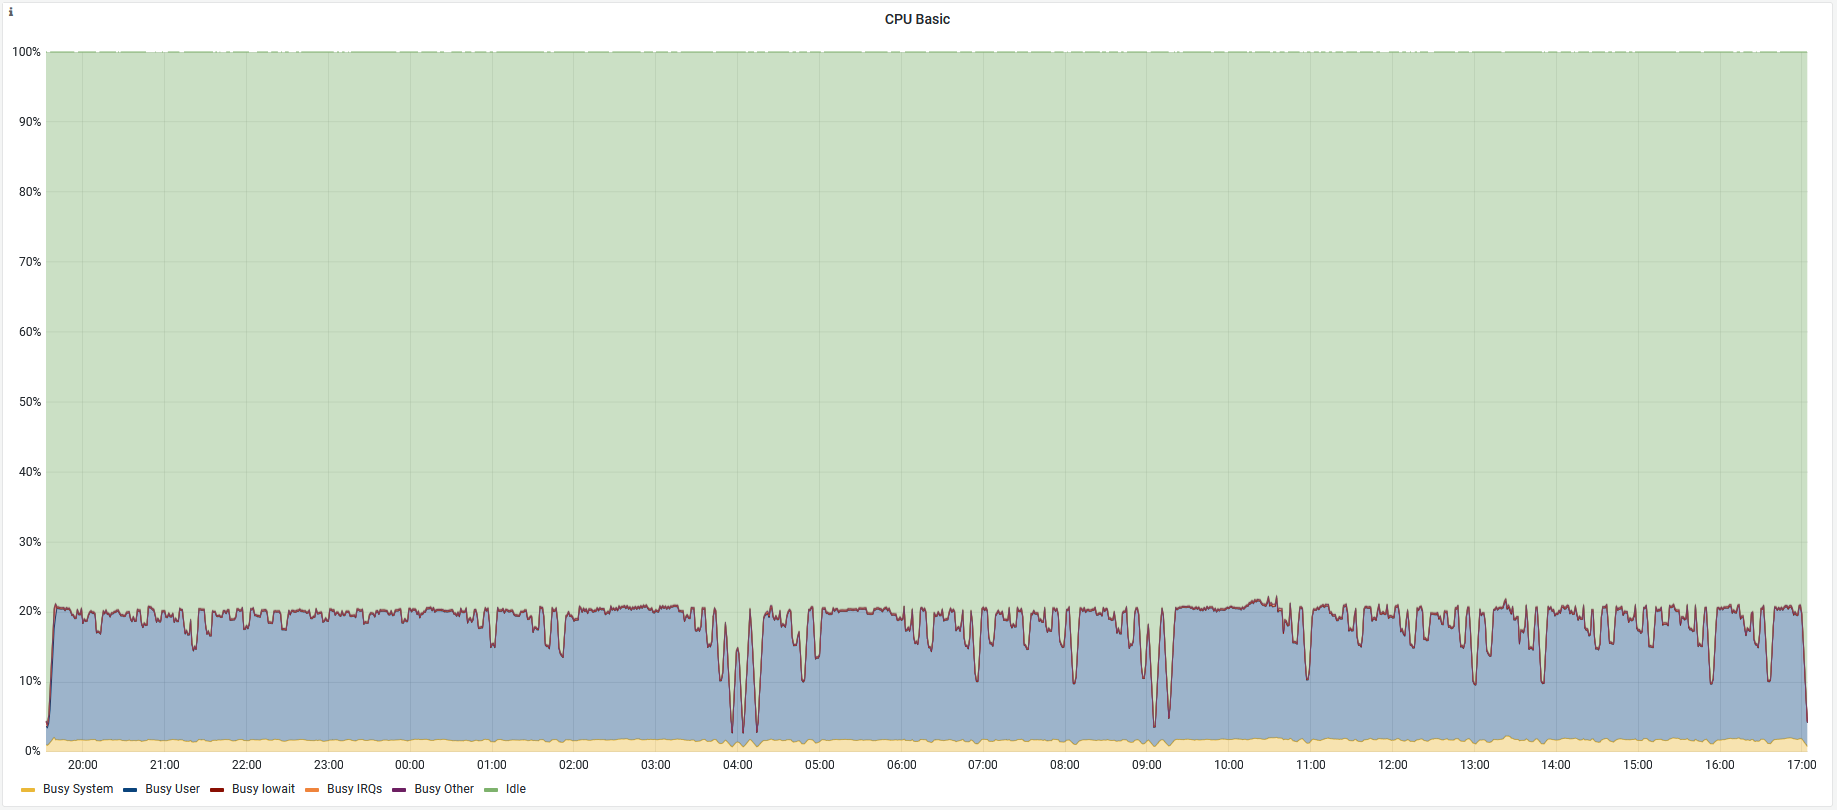
\includegraphics[width=1\linewidth]{other-fig/tests/cdf_cpu.png}
    \caption{...}
    % \label{fig:subjective_answers}
\end{figure}

\begin{figure}[H]
    \centering
    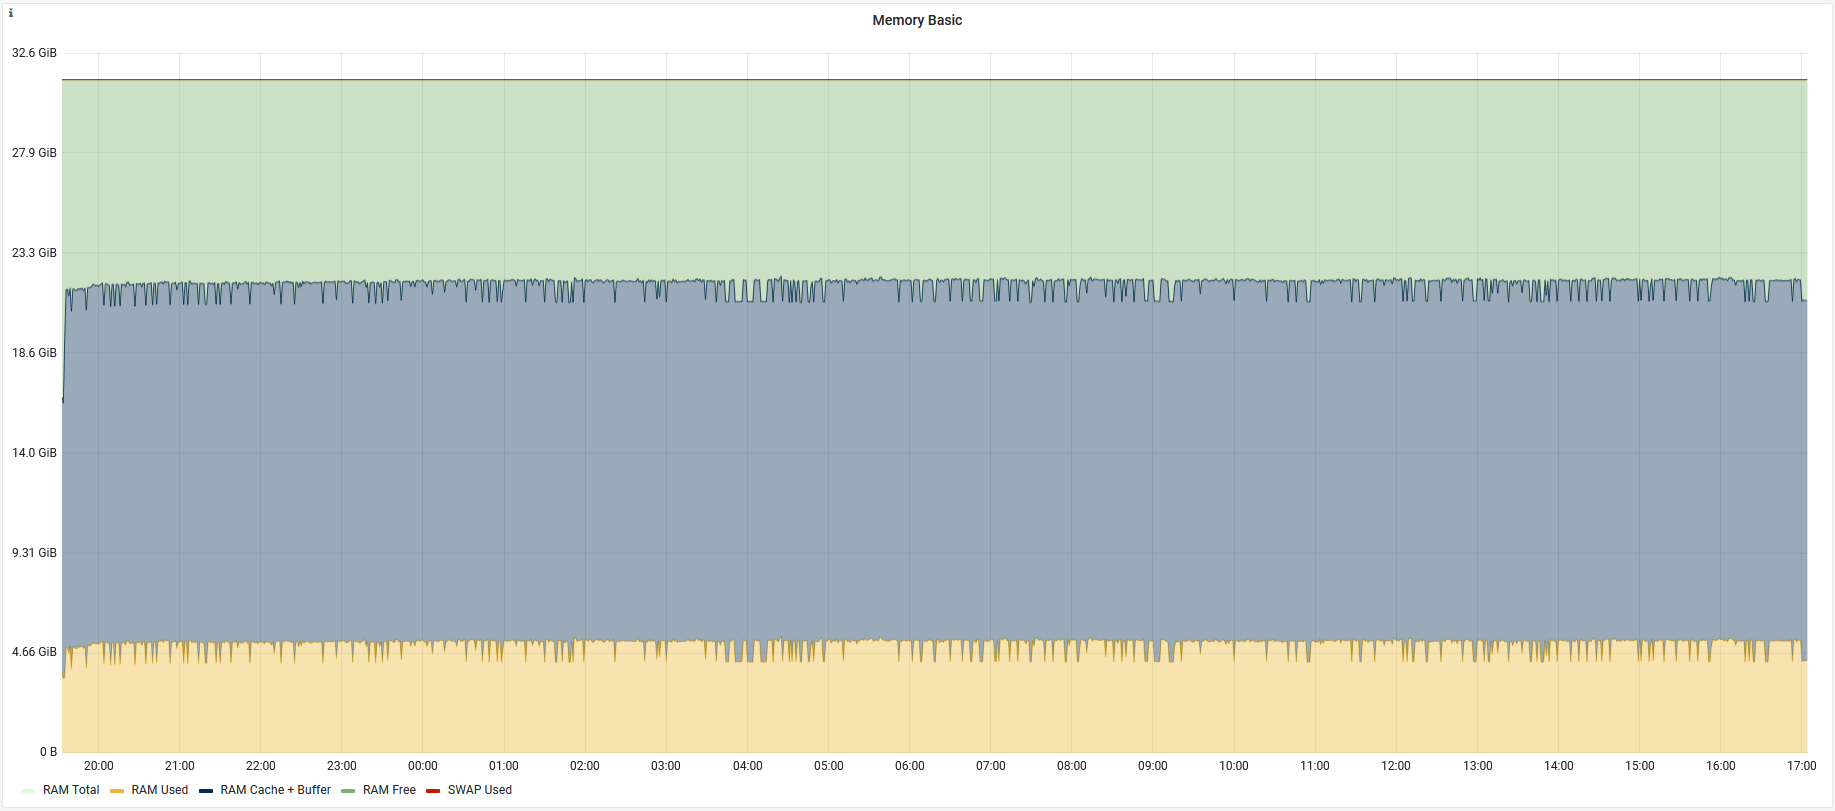
\includegraphics[width=1\linewidth]{other-fig/tests/cdf_ram.png}
    \caption{...}
    % \label{fig:subjective_answers}
\end{figure}

All files were processed by the framework, with a few exceptions where the file was not processed due to timeout. These were a couple of videos, compared to Deepware which did not process a large portion of the files, from a reliability perspective, the framework comes out better. The accuracy of the detection is questionable.

\section{Test case 2 - small bursts}

The second test no longer looked at the accuracy of the detection methods, but only at the resource usage in the workload. In this test, 100 files (25 videos and 75 audio recordings) were used. These files were shuffled and sent for detection in batches containing 5 files. Subsequently, all files were waited for evaluation before sending another batch.


\begin{figure}[H]
    \begin{subfigure}[h]{0.5\linewidth}
        \centering
        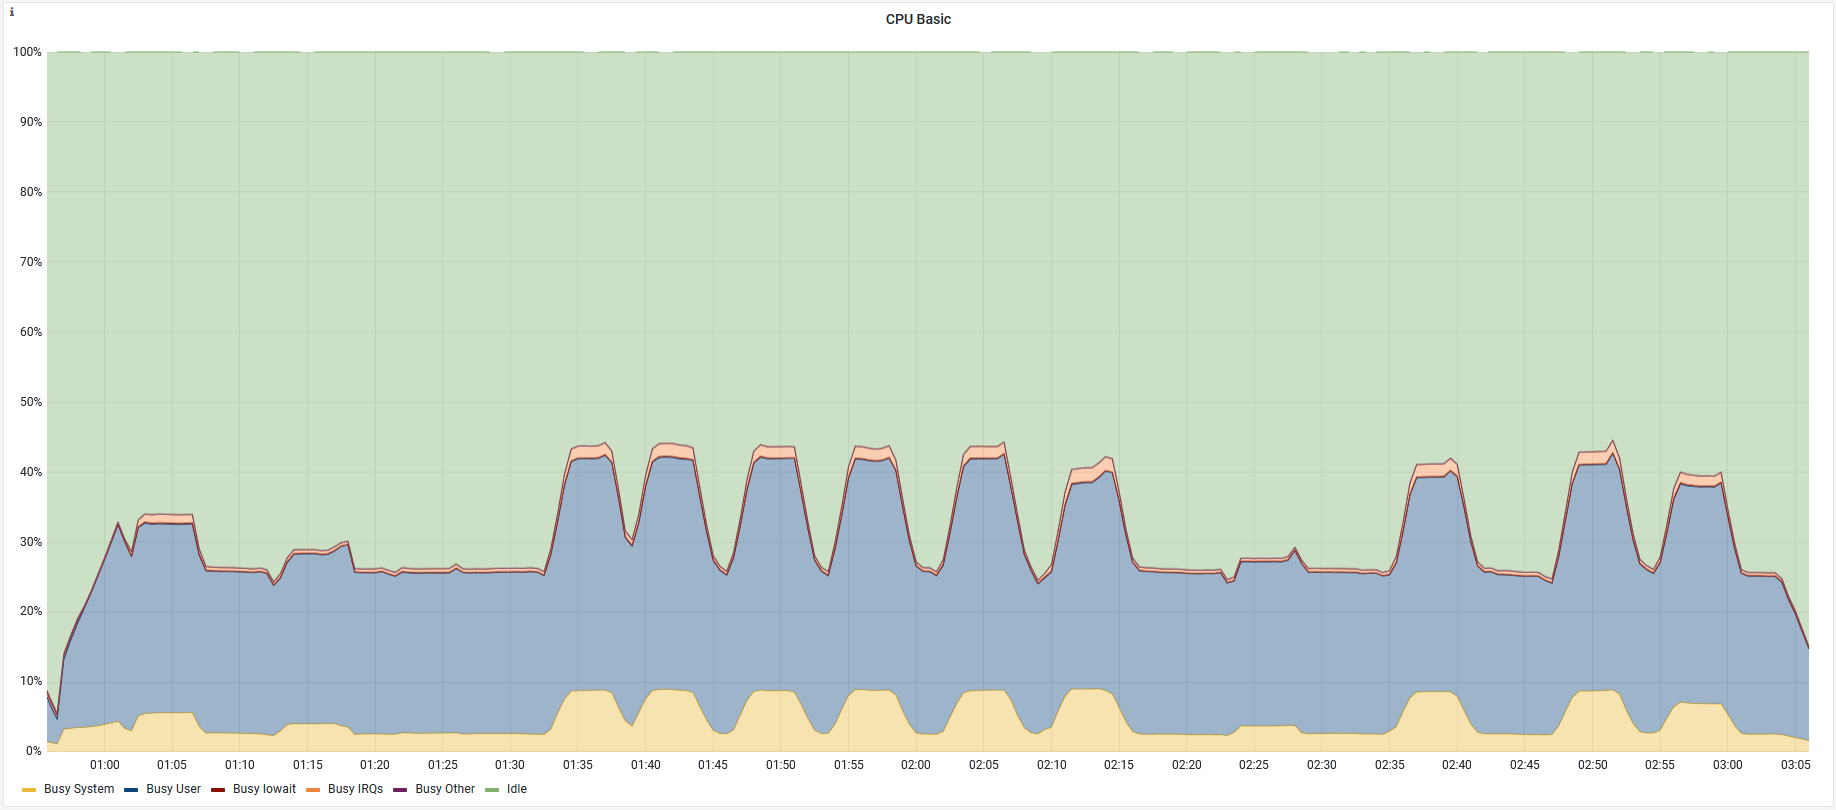
\includegraphics[width=1\linewidth]{other-fig/tests/burst_cpu1.png}
        \caption{...}
    \end{subfigure}
    \hfill
    \begin{subfigure}[h]{0.5\linewidth}
        \centering
        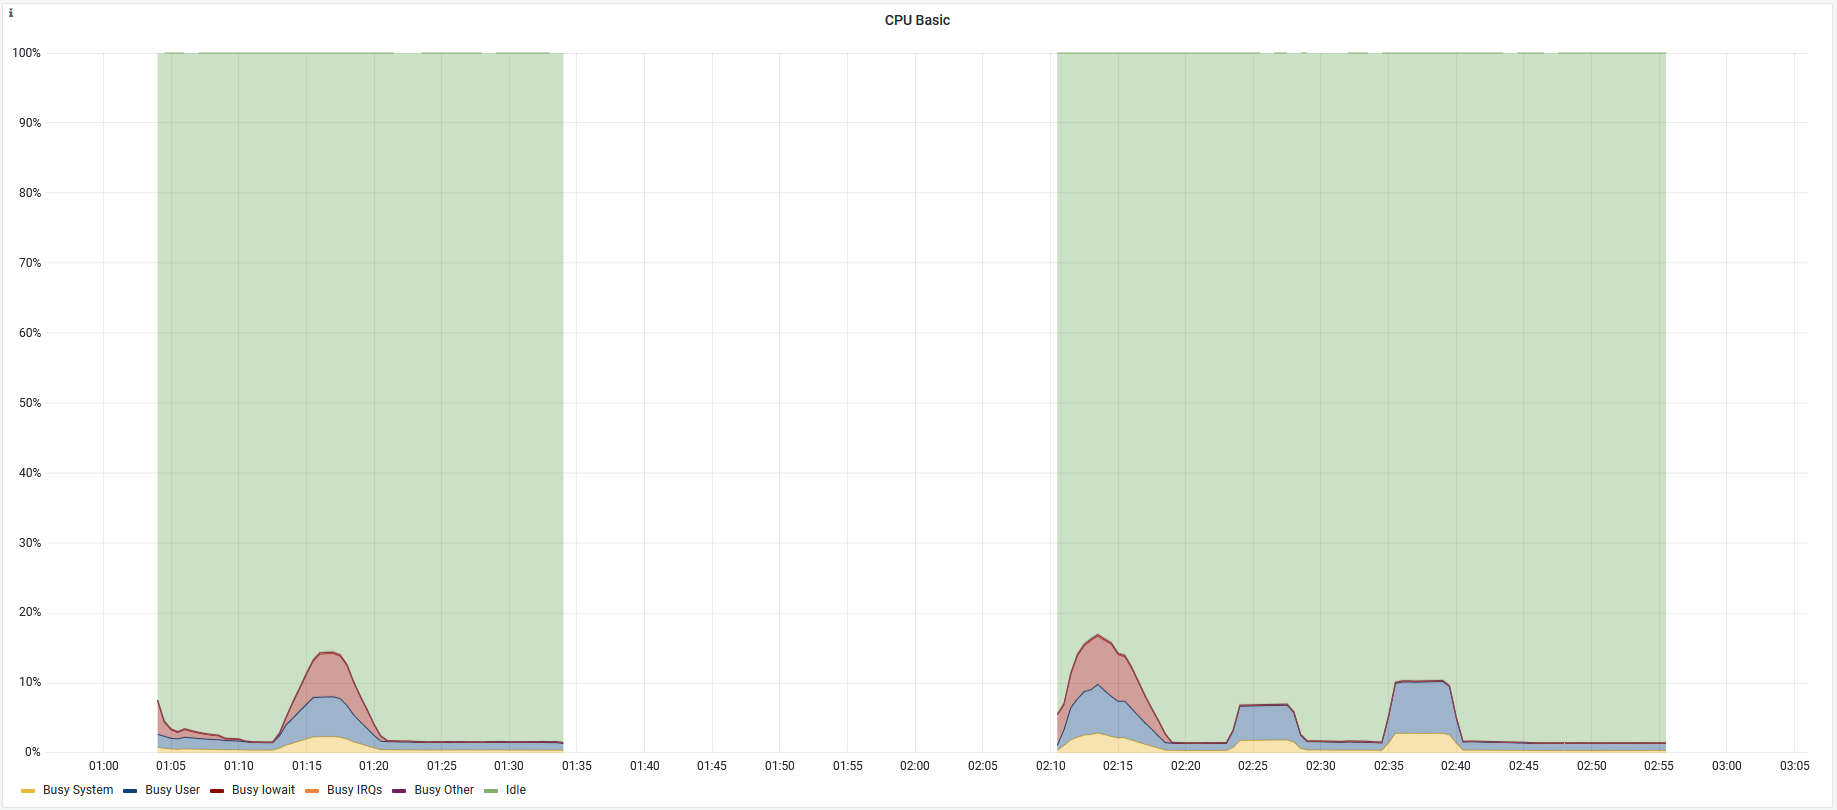
\includegraphics[width=1\linewidth]{other-fig/tests/burst_cpu2.png}
        \caption{...}
    \end{subfigure}
    \begin{subfigure}[h]{0.5\linewidth}
        \centering
        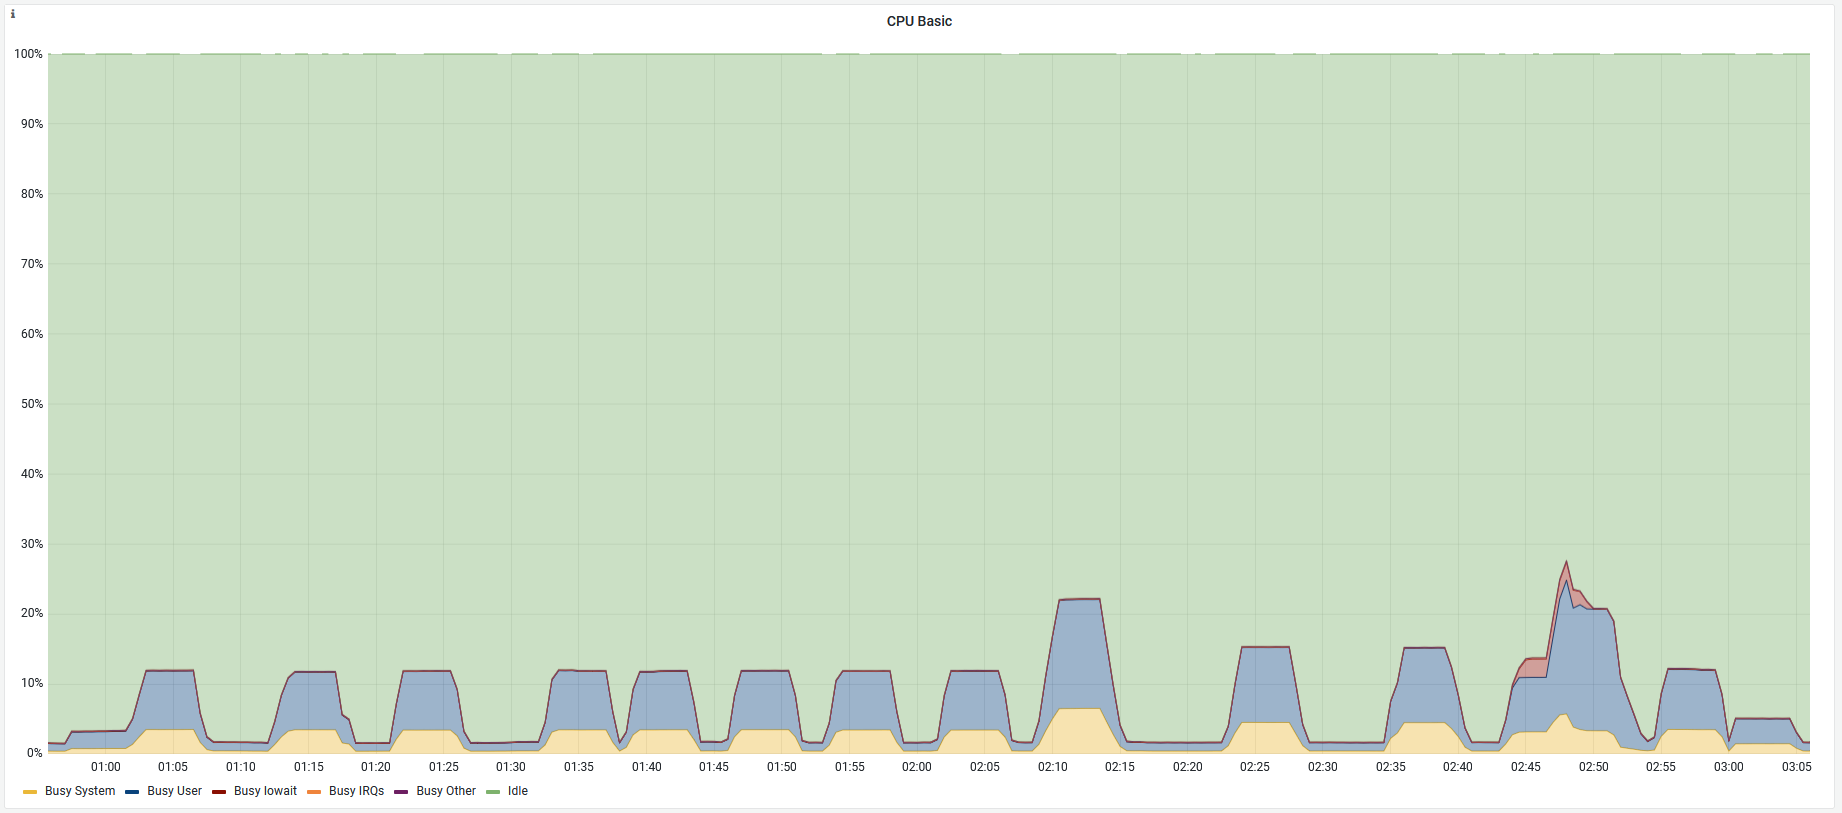
\includegraphics[width=1\linewidth]{other-fig/tests/burst_cpu3.png}
        \caption{...}
    \end{subfigure}
    \hfill
    \begin{subfigure}[h]{0.5\linewidth}
        \centering
        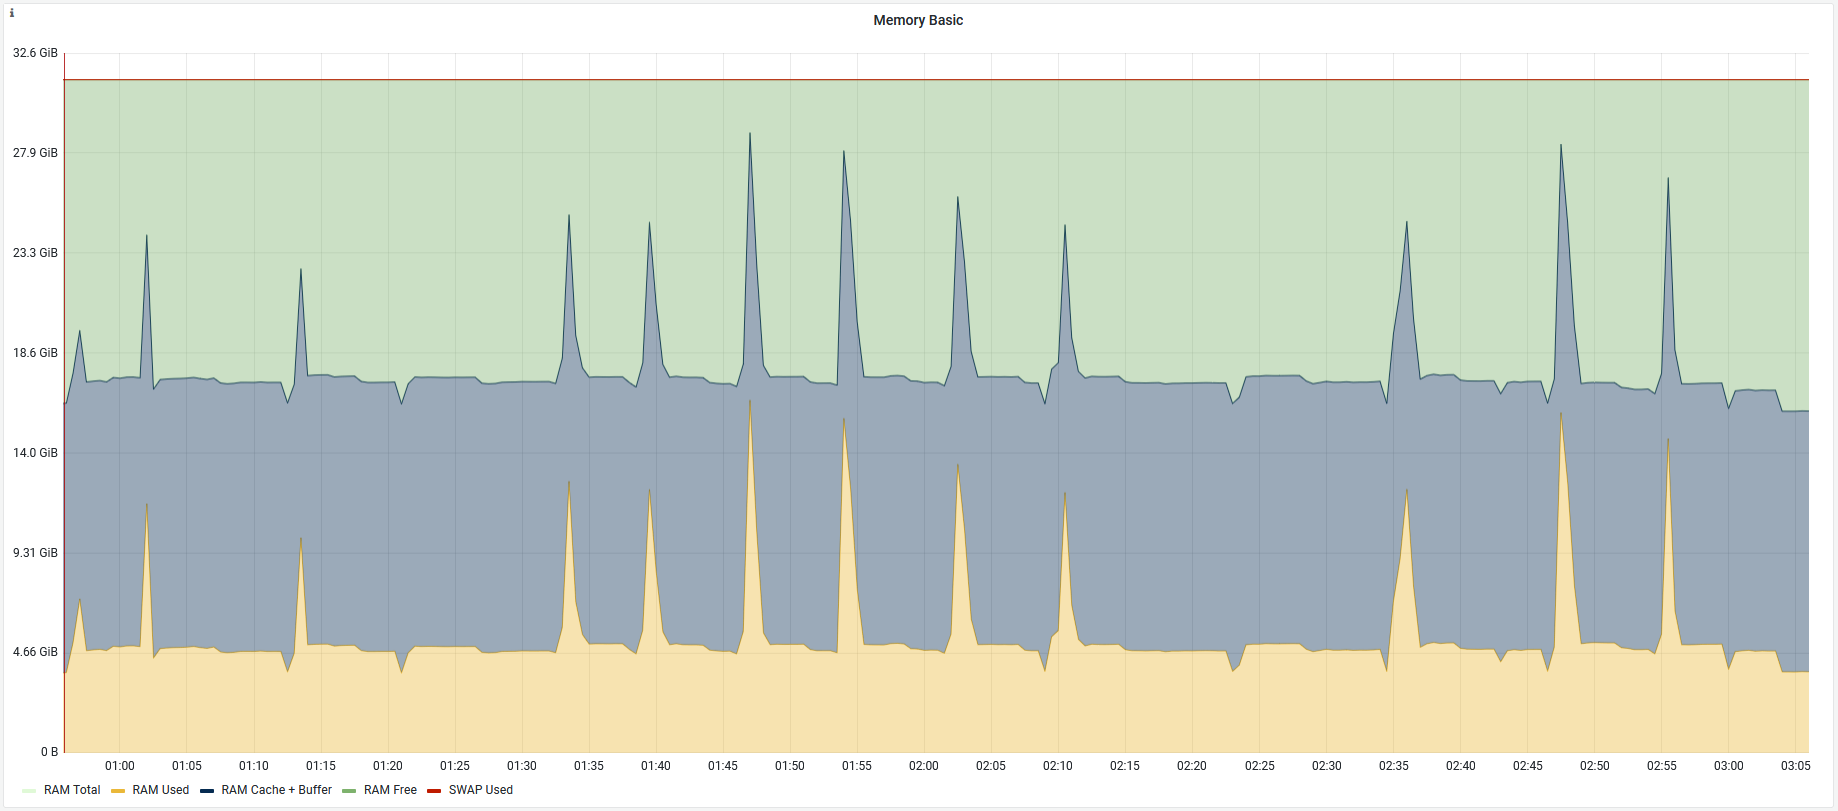
\includegraphics[width=1\linewidth]{other-fig/tests/burst_ram1.png}
        \caption{...}
    \end{subfigure}
    \caption{...}
    % \label{fig:subjective_answers}
\end{figure}

It took 2 hours 8 minutes to process all files. In the graphs, we can see that three nodes were used during the test. Not all of them worked all the time, but this fact confirms that the scaling works, the load was spread over multiple nodes, and in some cases the processing was done in parallel. Five files are borderline to effectively activate scaling, and these are more likely to be cases where 4 audio recordings and one video were sent for detection.

This test was repeated one more time to test if storing the results in the database would relieve the load on the system. This time the test lasted 2 minutes 41 seconds and according to the graphs the system hardly recognized that 100 files were detected.

\begin{figure}[H]
    \begin{subfigure}[h]{0.5\linewidth}
        \centering
        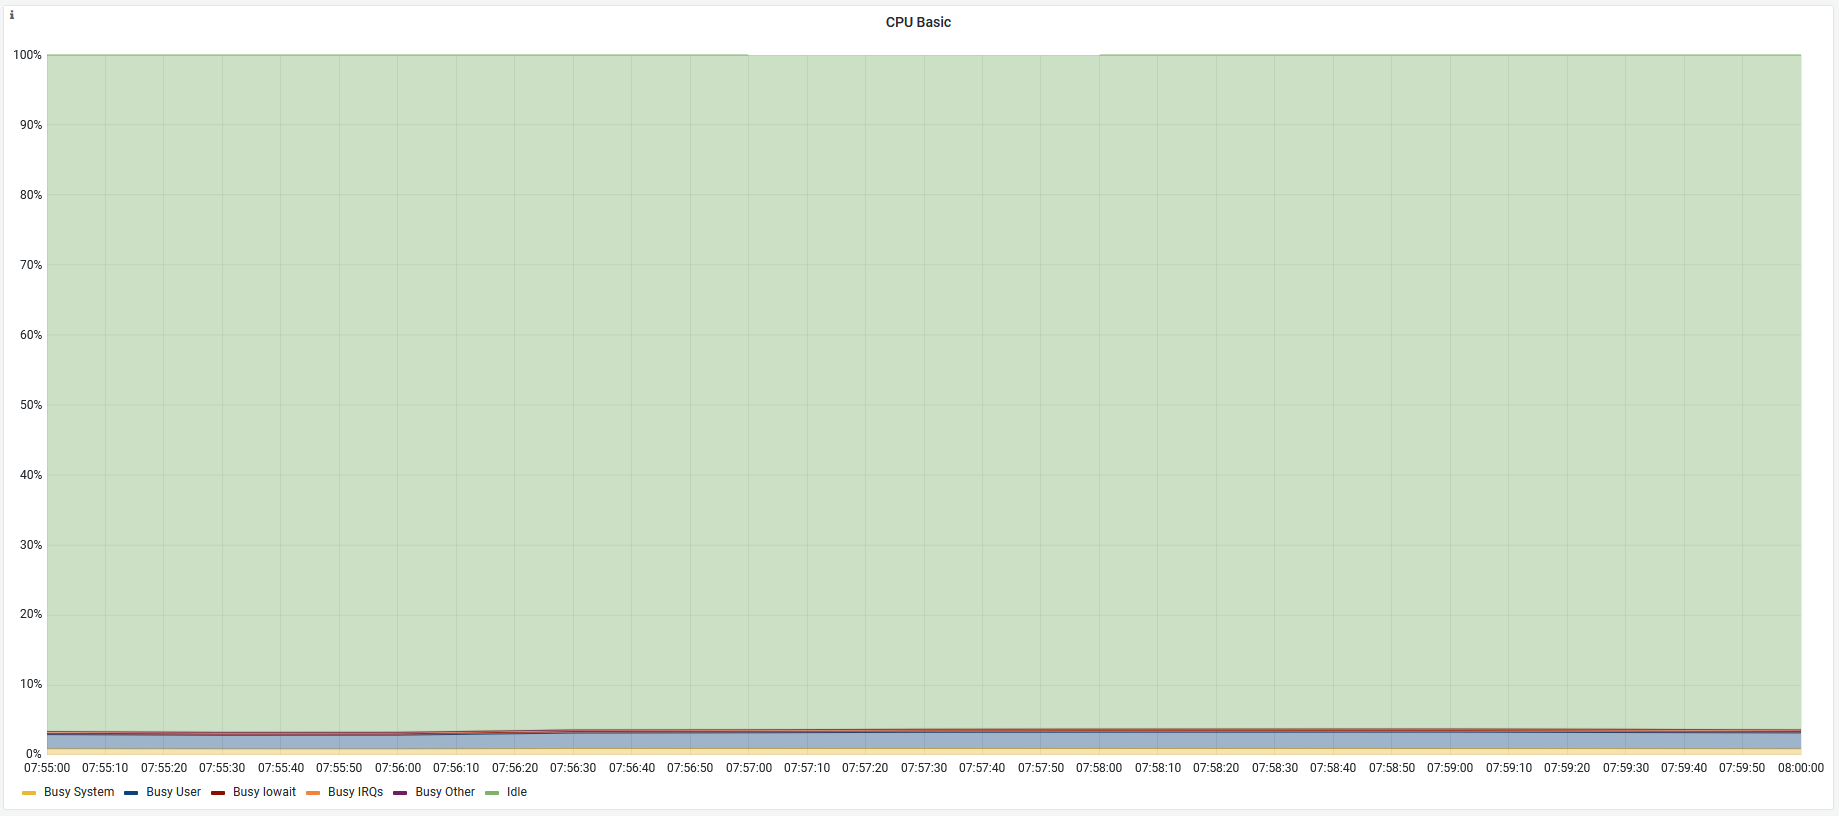
\includegraphics[width=1\linewidth]{other-fig/tests/burst_cached_cpu.png}
        \caption{...}
    \end{subfigure}
    \hfill
    \begin{subfigure}[h]{0.5\linewidth}
        \centering
        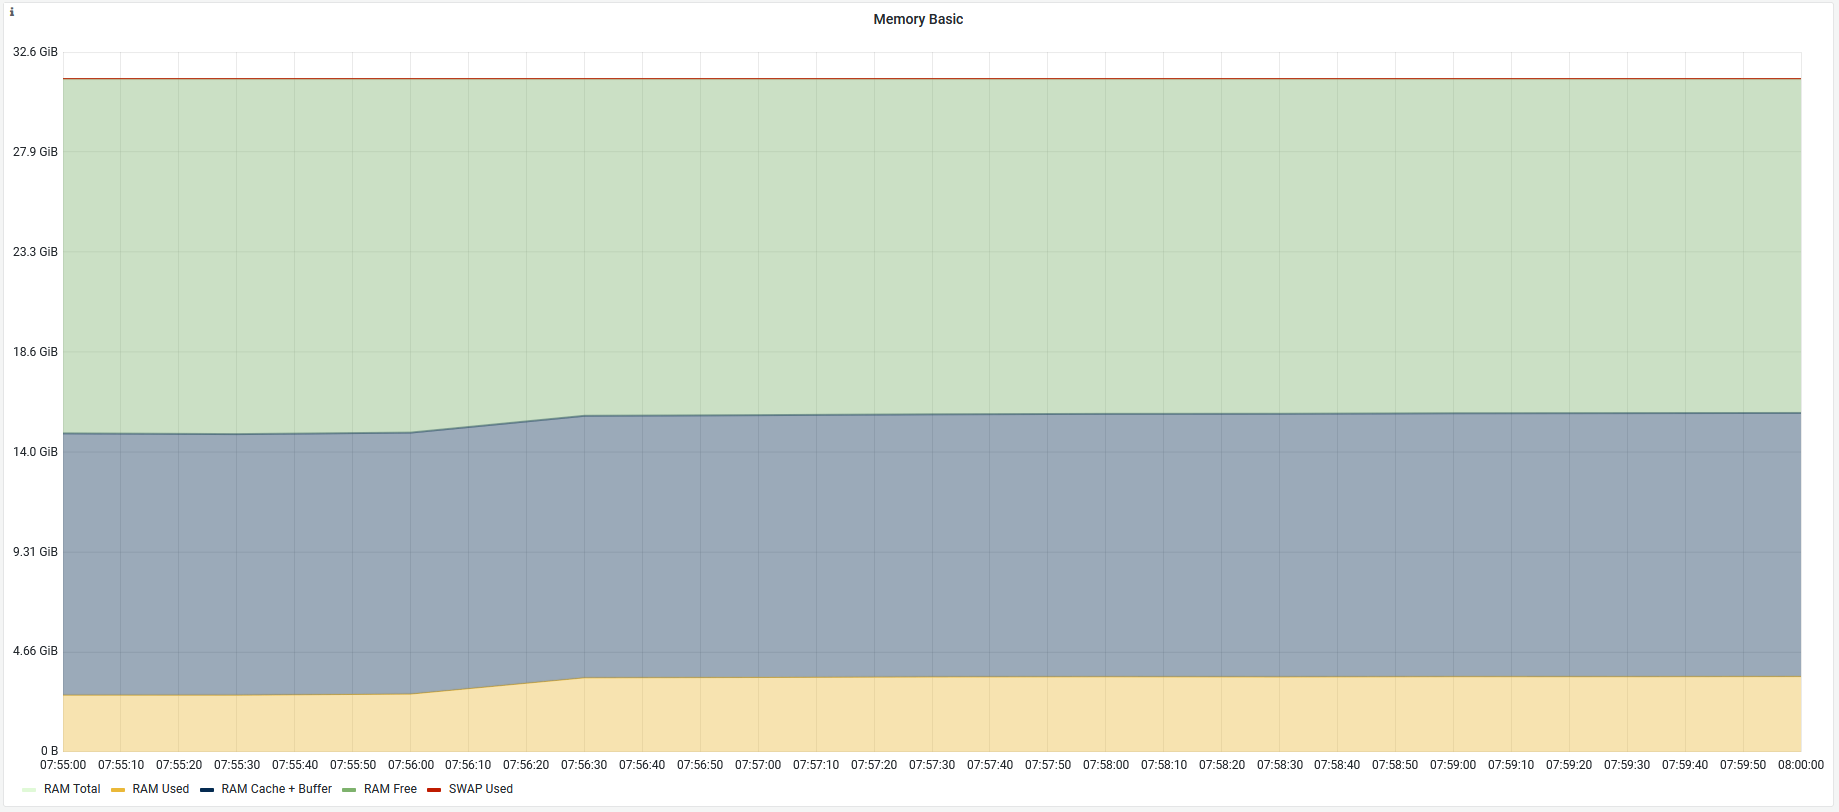
\includegraphics[width=1\linewidth]{other-fig/tests/burst_cached_ram.png}
        \caption{...}
    \end{subfigure}
    \caption{...}
    % \label{fig:subjective_answers}
\end{figure}

\section{Test case 3 - congestion}
The last test used the same data as the previous scenario; the dub was deleted so as not to use the already calculated results. In this scenario, all 100 files were sent at once to verify how the framework performs under load.

In this case, we can see that three nodes were activated and that the CPU load of all three was around 80 % for the time that the audio and video files were processed. Even though there were more audio files, the video processing took many times longer and we can observe that the load dropped dramatically in the middle, which lasted another few minutes. A similar trend can be seen for the RAM load. 

\begin{figure}[H]
    \begin{subfigure}[h]{0.5\linewidth}
        \centering
        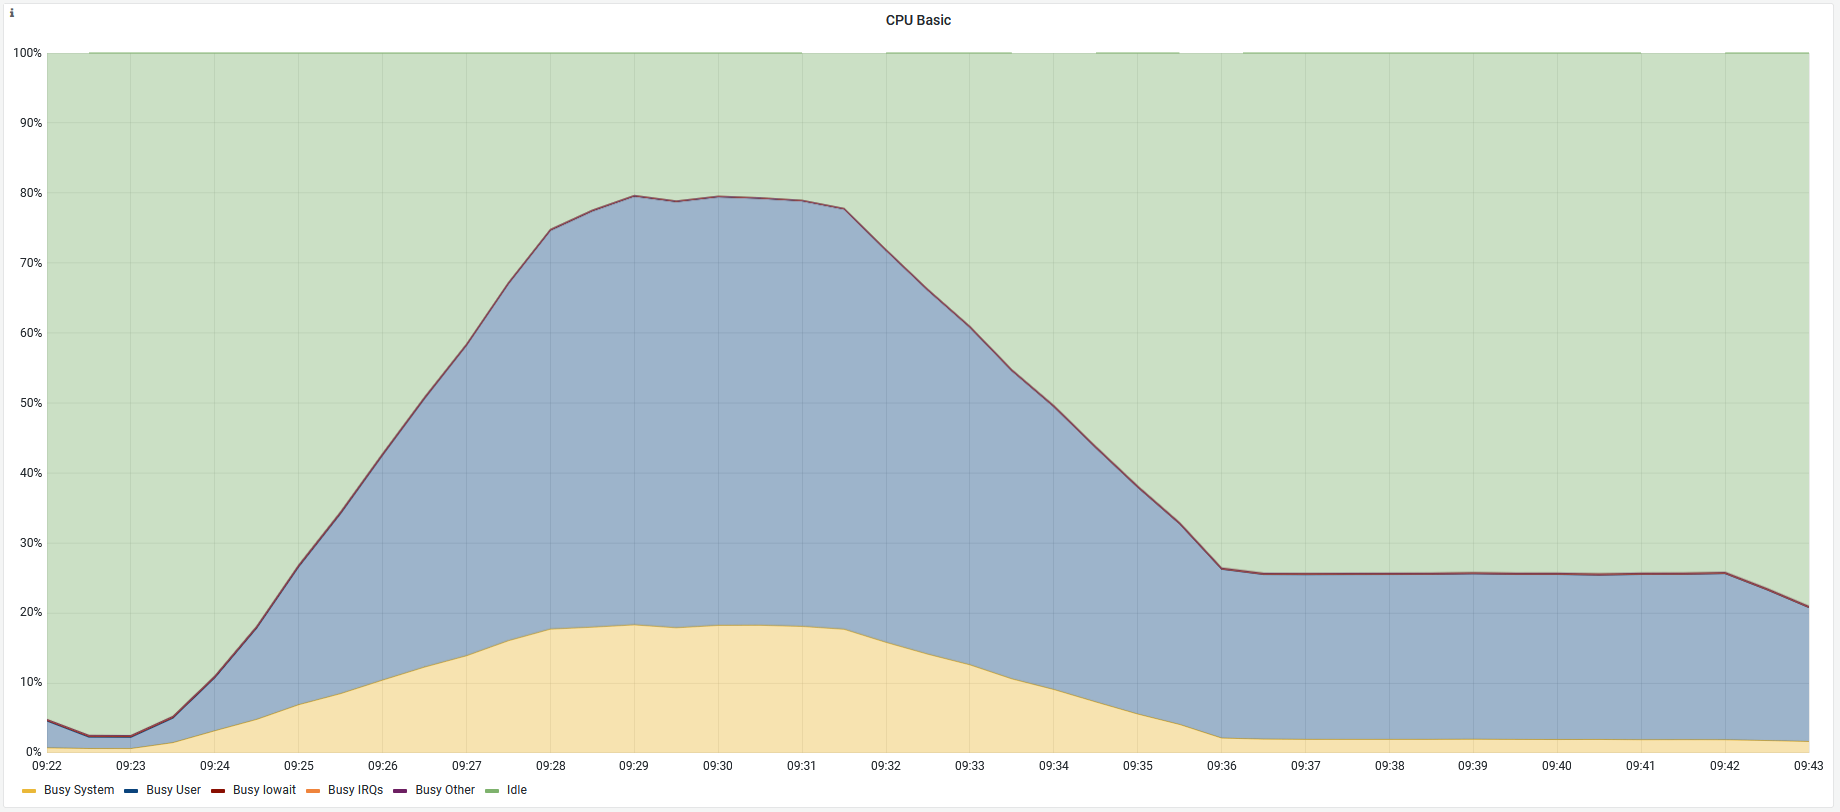
\includegraphics[width=1\linewidth]{other-fig/tests/overload_cpu1.png}
        \caption{...}
    \end{subfigure}
    \hfill
    \begin{subfigure}[h]{0.5\linewidth}
        \centering
        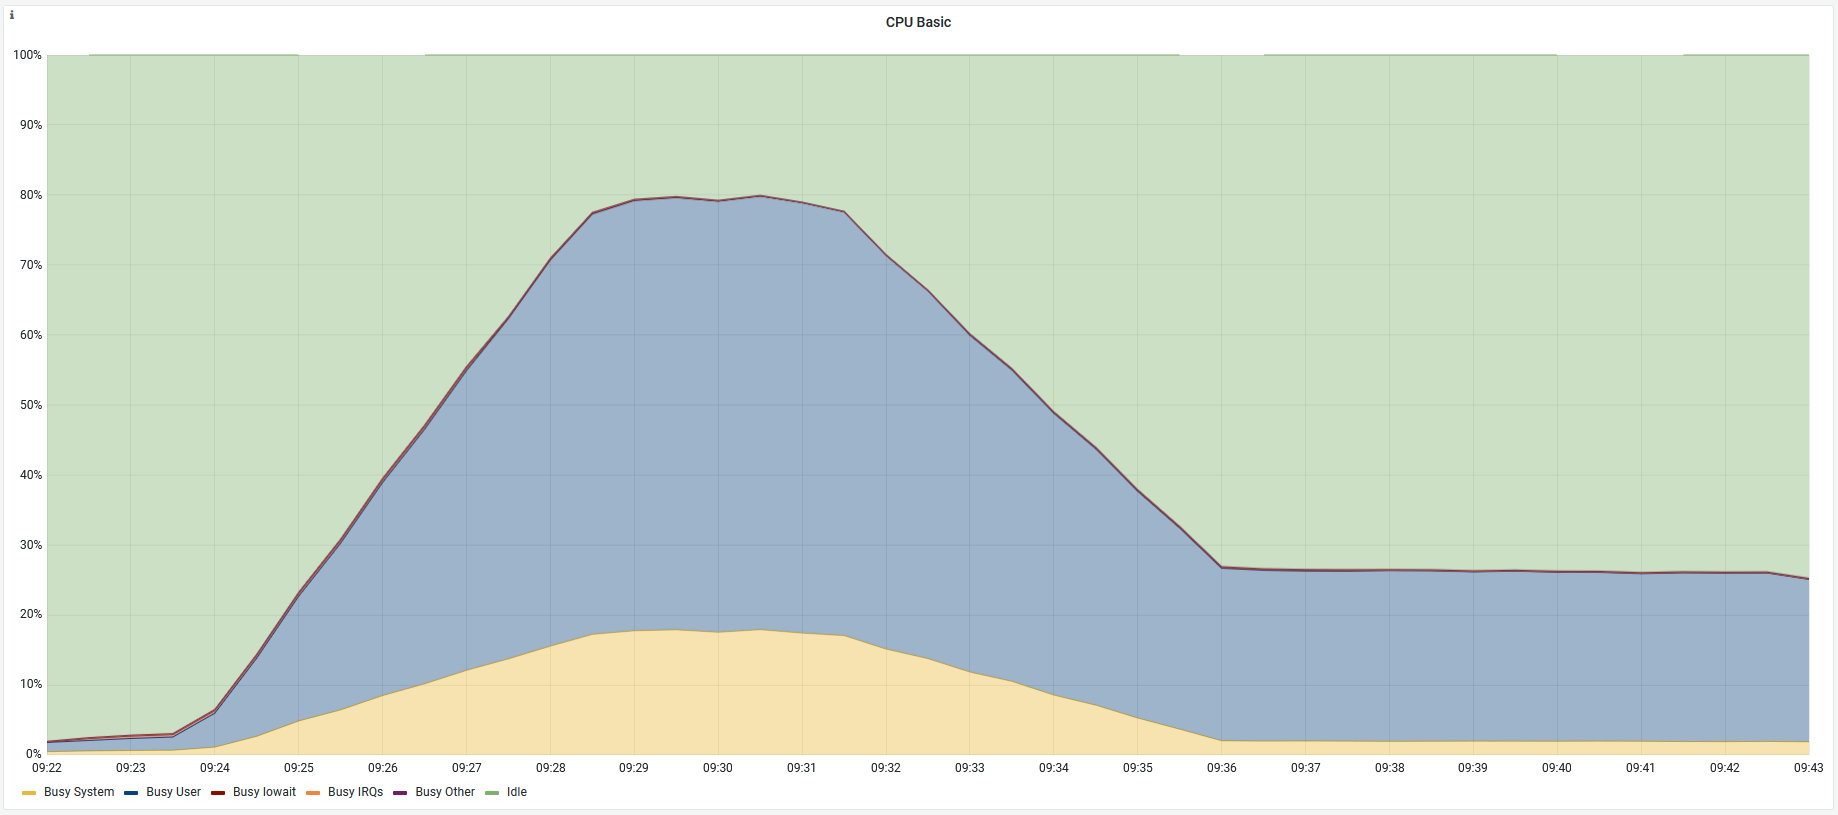
\includegraphics[width=1\linewidth]{other-fig/tests/overload_cpu2.png}
        \caption{...}
    \end{subfigure}
    \begin{subfigure}[h]{1\linewidth}
        \centering
        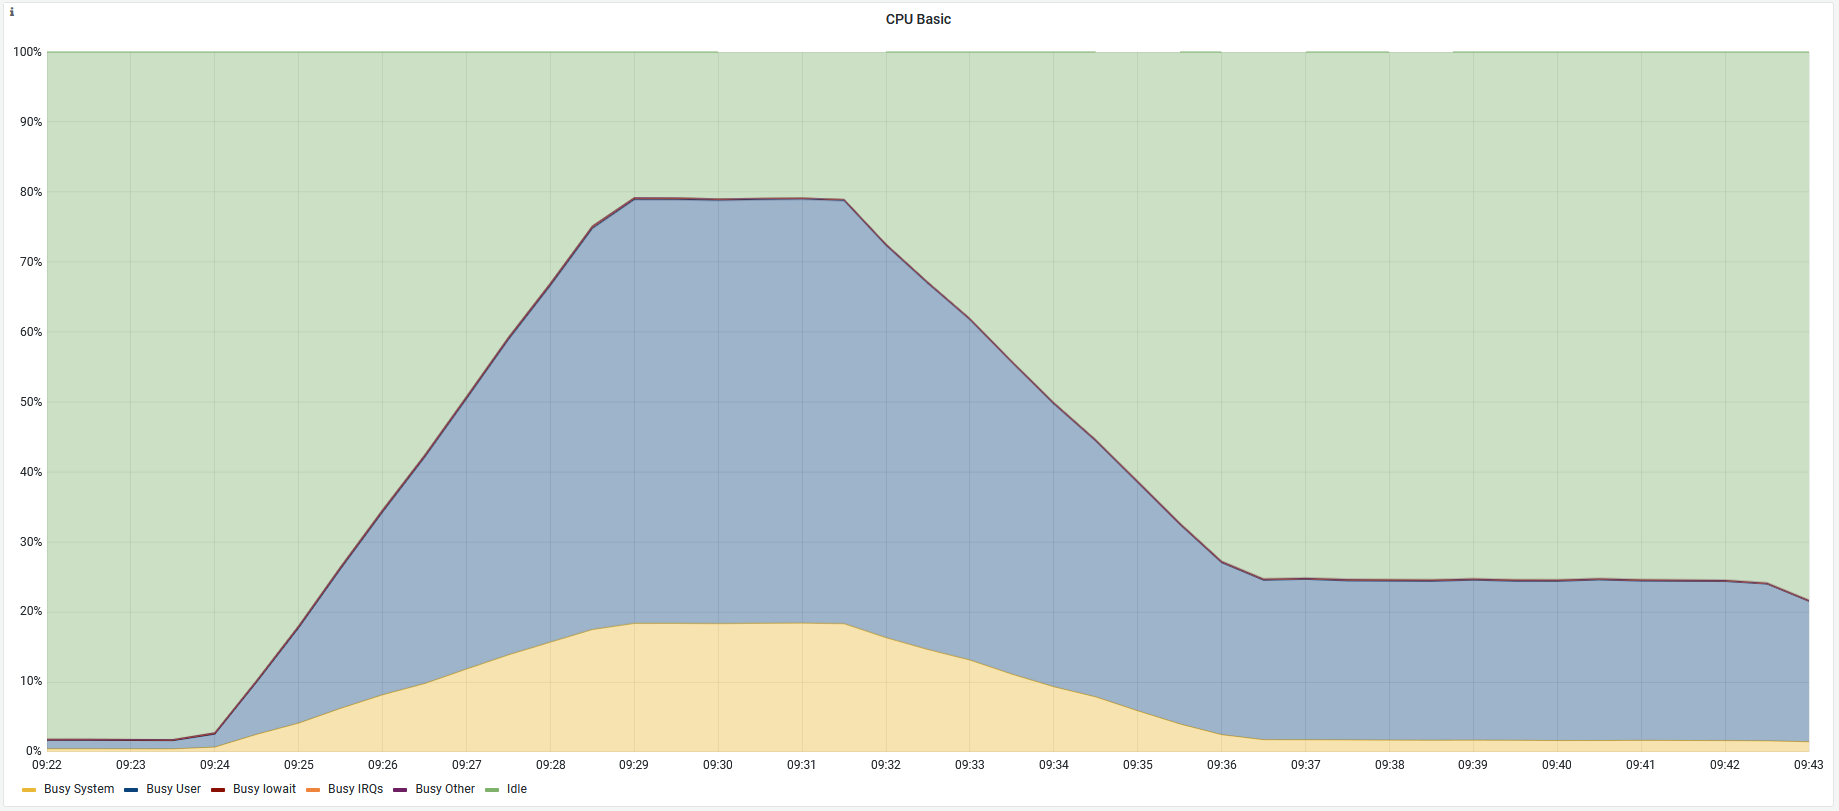
\includegraphics[width=0.5\linewidth]{other-fig/tests/overload_cpu3.png}
        \caption{...}
    \end{subfigure}
    \caption{...}
    % \label{fig:subjective_answers}
\end{figure}

The framework was able to process all 100 files in a time of 19 minutes, 31 seconds. This is a rapid acceleration over the previous scenario. We can observe that the scaling of the system is fast and helps the processing speed under load to be very substantially.

\begin{figure}[H]
    \begin{subfigure}[h]{0.5\linewidth}
        \centering
        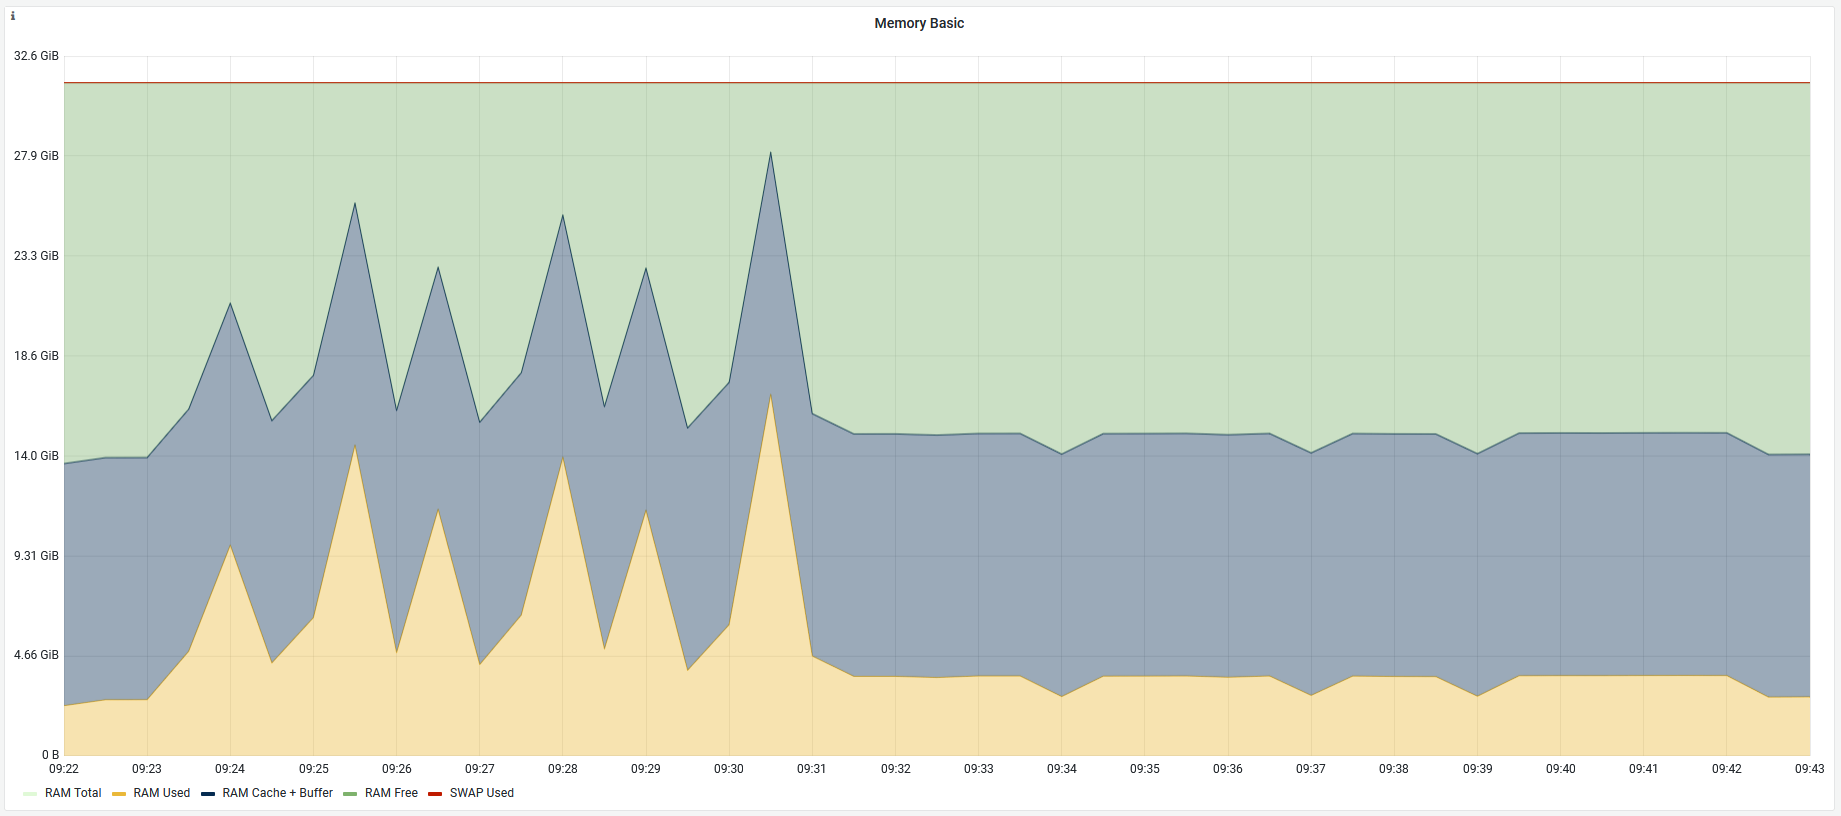
\includegraphics[width=1\linewidth]{other-fig/tests/overload_ram1.png}
        \caption{...}
    \end{subfigure}
    \hfill
    \begin{subfigure}[h]{0.5\linewidth}
        \centering
        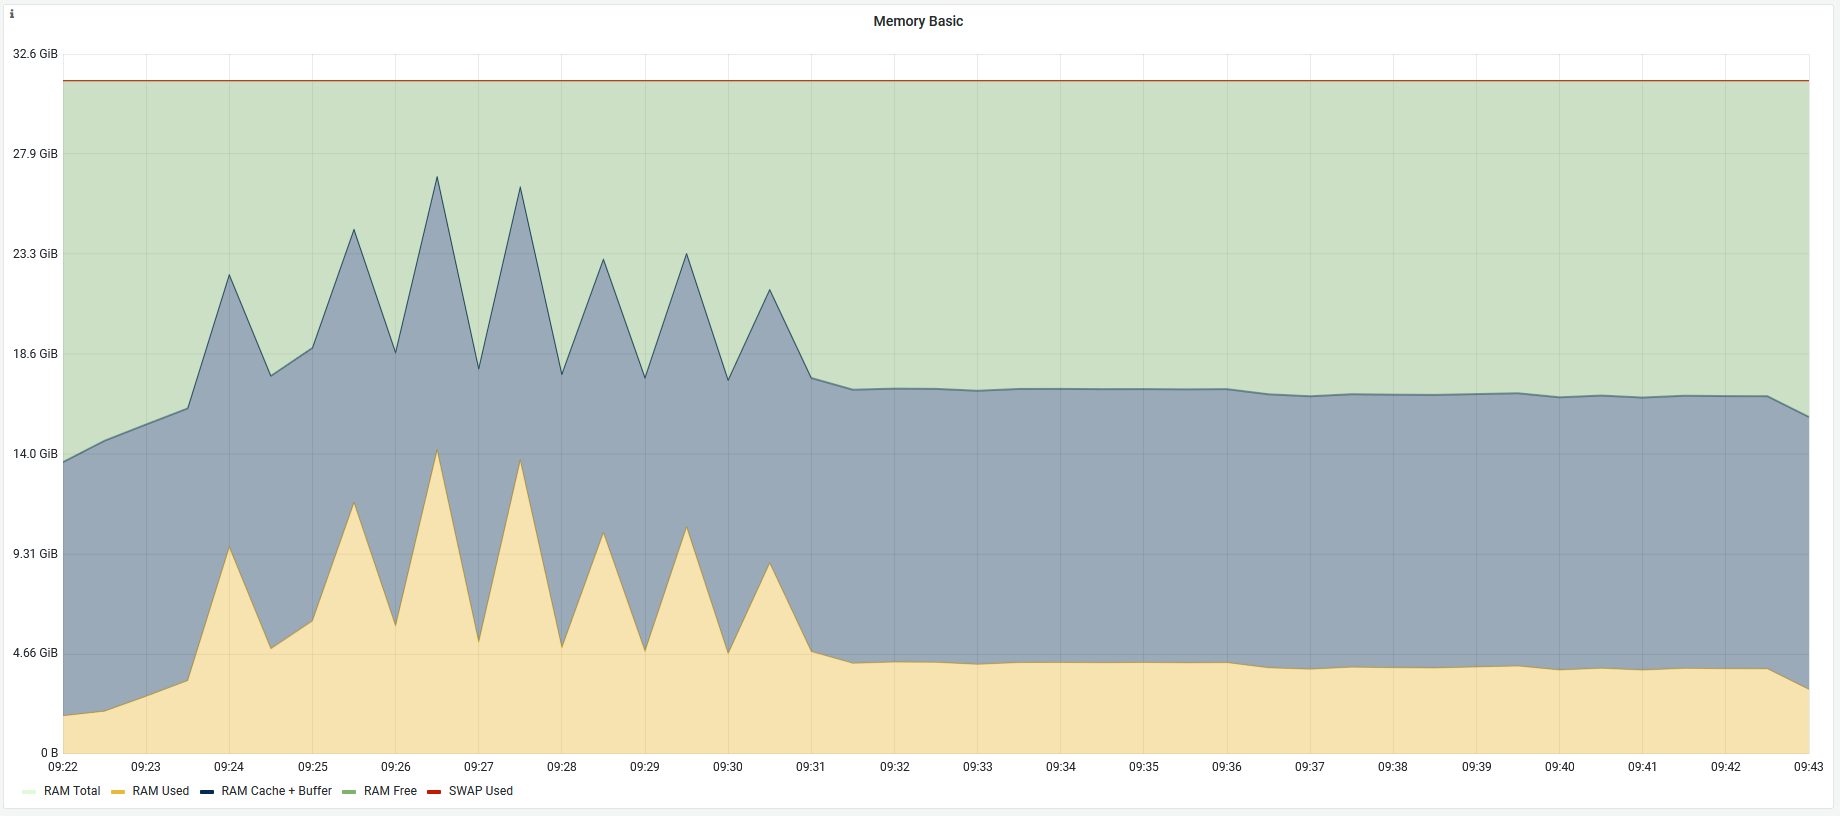
\includegraphics[width=1\linewidth]{other-fig/tests/overload_ram2.png}
        \caption{...}
    \end{subfigure}
    \begin{subfigure}[h]{1\linewidth}
        \centering
        \includegraphics[width=0.5\linewidth]{other-fig/tests/overload_ram3.png}
        \caption{...}
    \end{subfigure}
    \caption{...}
    % \label{fig:subjective_answers}
\end{figure}

\section{Tests evaluation}

In the first scenario, we can see that the system is not efficiently loaded and resources are being wasted. At first glance it may look like this, but each method has access to a limited amount of resources, so when the system is under load it will work reliably. Therefore, sequential utilization is not appropriate.

Kuberentes can be set up to have individual containers contend for resources, but this greatly increased the management overhead of the system and did not produce a performance jump. The resource allocation can be easily changed, and certainly the system could be set up better based on these tests. It will also depend greatly on the particular HW that will be realistically used. The framework setup has to be tailored to the system. Still, the system works reliably, and especially its good features will only show up in a real workload.

The system had to run with 32 GB of RAM; otherwise, the audio detection methods failed because of lack of memory. Each method must have at least 3 GB of memory guaranteed, better a bit more. All methods run in parallel at the same time, which puts a lot of demands on the host platform. This problem could be fixed by changing the Controller so that all six detection methods do not run in parallel but in smaller batches. This would increase the processing time, but it would be possible to run on a platform with 16 GB of RAM. Scaling would then also be more efficient.

The video detection method was not very fast in processing, so I would not recommend it for use in the production version. Some optimizations would need to be made. Audio detection methods on the other hand did not provide great detection accuracy, this could be changed by using a more robust dataset to train.

Although the individual methods did not achieve high quality, the implementation and tests can be declared successful. The framework can perform its work reliably for several hours and the scaling efficiency becomes apparent under load. As a result, the framework is able to handle a large number of files in a relatively short time. The only problem is the use of more powerful HW when integrating a large number of methods, this could be partially reduced by changing the Conteroller or possibly optimizing individual methods. The deployment of the framework strongly depends on the integrated methods and, accordingly, the HW used. 

\section{Cost analysis}

The framework required HW with 32 GB of RAM for its functionality, and the use of neural networks is a computationally demanding operation; it was also necessary to have at least 4 CPUs available. In the end, the B8ms virtual machine was chosen for deployment in Azure AKS. This machine provides 8 CPUs, 32 GB RAM and costs \$0.38 per hour to operate. 

A system with no load needs one such machine, but if there is a load and scaling is applied, there may be more of these machines running. In our case, we have set the maximum number of nodes to 3. Therefore, if the framework were at 100 \% load, an hour of three of these machines would cost \$1.14. The framework also requires external IP, a load balancer, and storage. These items in our case cost a tenth of what virtual machines cost.

In testing that ran for several days and scaling was applied at certain stages, one day of running this framework cost about \$18.8 on average. That would work out to a monthly operation of \$564. In our case, we were using a free cluster that is designed for development and testing. The standard cluster is chargeable but provides a more stable environment that is focused on speed, availability, and reliability. The cost of the standard cluster is \$70, so the total cost would be over \$600 per month.

If a machine with only 16 GB of RAM could be used and more scaling could be utilized, savings could be realized while maintaining similar features. Alternatively, utilize a custom HW, where the purchase price of the HW and its potential lifetime, maintenance, and cost of operation would have to be factored into the price. 

% ----------------------------------------------------------------------- %
\chapter{Conclusion}
everythings implemented and it is working, :)

